%%%%%%%%%%%%%%%%%%%%%%%%%%%%%%%%%%%%%%%%%%%%%%%%%%%%%%%%%%%%%%%%%%%%%
%%%                       ANALYSIS OVERVIEW                       %%%
%%%%%%%%%%%%%%%%%%%%%%%%%%%%%%%%%%%%%%%%%%%%%%%%%%%%%%%%%%%%%%%%%%%%%
\section{Event selection}\label{sec:EventSelection}
%Introduction:
We are searching for \gls{nuone} elastic scattering events, characterised by a single very forward going electron shower, specifically focusing on low electron recoil energies. The main backgrounds for our analysis come from $\nu_e$\gls{CC} interactions, which produce an electron with additional activity, and interactions that produce $\pi^0$, which decays into two photons producing electromagnetic showers, where each can look similar to the \gls{nuone} signal. Additionally, there are $\nu_\mu$\gls{CC} interactions, which are generally easy to distinguish from our signal, however, their very high abundance in the \gls{NOvA} \gls{ND} makes them a dominant background nevertheless.


A summary of the true cuts used for the selection of the individual signal and background samples is shown in Tab.~\ref{tab:NuMMSamplesSelection}. The signal definitions use the \texttt{kMode} variable instead of the \texttt{kIntType}, which is now deprecated (ref.: various Slack conversations). Mode 10005 denotes only the \gls{nuone} events and is only available for the enhanced \gls{nuone} samples, while mode 5 denotes all electron scattering events, including inverse muon decay interactions. That is why we had to add a requirement of an electron in the final state. The \texttt{kIsNueCCMEC} is defined as \texttt{kMode===10}, which denotes all Meson Exchange Current (MEC) events, at the same time as \texttt{kIsNue} and \texttt{kIsCC}.

\begin{table}[!ht]
\centering
\caption{Overview of the true cuts used to selection the signal and background samples.}
\def\arraystretch{1.4}
\begin{tabular}{l@{\hskip 1cm}l@{\hskip 1cm}l@{\hskip 1cm}l}
Signal type            & Selection\\\hline
Signal                 & \texttt{kIsVtxContained} \&\& $\texttt{kMode}==10005$\\
\gls{nuone} background & $\texttt{kMode}==10005$\\
$\nu_e$\gls{CC} \gls{MEC} background & $!\left(\texttt{kMode}==5\text{ \&\& }\texttt{kHasElInFinState}\right)$  \&\& \texttt{kIsNueCCMEC}\\
Other background       & $!\left(\texttt{kMode}==5\text{ \&\& }\texttt{kHasElInFinState}\right)$  \&\& !\texttt{kIsNueCCMEC}
\end{tabular}
\label{tab:NuMMSamplesSelection}
\end{table}

We explain the motivation behind each cut of the event selection and discuss their effect on the neutrino magnetic moment events below. We also consider possible improvements to the event selection for a future (re-)analysis.

The strategy for event selection is as follows. First, we remove events that failed reconstruction or data collection, described in Sec.~\ref{sec:NuMMEventSelSpillCuts} and \ref{sec:NuMMEventSelRecoQC}. Then, we apply pre-selection cuts that remove obvious background (Sec.~\ref{sec:NuMMEventSelectionPresel}), while limiting the reduction of the signal efficiency to about $\unit[0.25]{\%}$. Following this, we apply the containment cuts (Sec.~\ref{sec:NuMMEventSelFidCont}) that remove events that are either not fully contained within the detector, or events that originate from outside of the detector, such as rock muons. Afterwards, we perform a cut-based \gls{MVA} on a selection of variables useful for distinguishing the signal from the background, discussed in Sec.~\ref{sec:NuMMEventSelTMVA}, and evaluate their combined performance on the signal selection. We choose the cut values that result in the best statistical significance, based on a chosen \gls{FOM}. Given that we are searching for a very limited number of signal events on top of a large background, we chose a simple statistics-only \gls{FOM}
\begin{equation}\label{eq:NuMMFOM}
\textsf{\gls{FOM}} = \frac{\textsf{Signal}}{\sqrt{\textsf{Background}}}.
\end{equation}

The summary of the cut values for the event selection of neutrino magnetic moment signal is presented in Tab.~\ref{tab:EventSelectionSummary}, showing the label for the event selection variable, its description and the cut value chosen. After the full event selection, the predicted number of signal events for $\mu_\nu=10^{-9}\mu_B$ is $56.80$ and the total number of background events under the \gls{SM} hypothesis is $700.33$.

\begin{table}[!hb]
\centering
\caption[Event selection summary]{Summary of the variables and their cut values for the event selection of neutrino magnetic moment signal. Showing the category of the event selection variable, its label, description and the cut value chosen.}
\begin{tabular}{|m{2mm} m{0.15\textwidth} m{0.53\textwidth} m{0.21\textwidth}|}\hline
& \textbf{Label} & \textbf{Description} & \textbf{Cut} \\\hline
\parbox[t]{2mm}{\multirow{5}{*}{\rotatebox[origin=c]{90}{\textbf{Reco Qual.}}}} &
\textbf{Valid Vtx} & Valid reconstructed vertex & $>0$\\
& \textbf{N$^o$ Prongs} & Number of reconstructed prongs & $>0$\\
& \textbf{Hits / Plane} & Number of hits per plane & $<6$\\
& \textbf{Low $E_{Shower}$} & Low cut on calorimetric energy of the most energetic shower & $>\unit[0.5]{GeV}$\\\hline
\parbox[t]{2mm}{\multirow{4}{*}{\rotatebox[origin=c]{90}{\textbf{Preselection}}}} &
\textbf{N$^o$~Hits Loose} & Preliminary cut on the total number of hits for all prongs in a slice & $<280$\\
& \textbf{Prong Length} & Length of the longest prong & $<\unit[640]{cm}$\\
& \textbf{$E\theta^2$ Loose} & Preliminary cut on the product of the calorimetric energy and angle squared of the leading shower & $<0.064\unit{GeV\times rad^2}$\\\hline
\parbox[t]{2mm}{\multirow{6}{*}{\rotatebox[origin=c]{90}{\textbf{Fiducial}}}} &
\multirow{6}{*}{\textbf{Vertex}} & \multirow{2}{*}{x position} & $>\unit[-177]{cm}$\\
& & & $<\unit[177]{cm}$\\
& & \multirow{2}{*}{y position} & $>\unit[-177]{cm}$\\
& & & $<\unit[177]{cm}$\\
& & \multirow{2}{*}{z position} & $\unit[>50]{cm}$\\
& & & $<\unit[1170]{cm}$\\\hline
\parbox[t]{2mm}{\multirow{6}{*}{\rotatebox[origin=c]{90}{\textbf{Containment}}}} &
\multirow{6}{*}{\textbf{Prong}} & Minimum hit position in x & $>\unit[-177]{cm}$\\
& & Maximum hit position in x & $<\unit[177]{cm}$\\
& & Minimum hit position in y & $>\unit[-185]{cm}$\\
& & Maximum hit position in y & $<\unit[177]{cm}$\\
& & Minimum hit position in z & $>\unit[55]{cm}$\\
& & Maximum hit position in z & $<\unit[1270]{cm}$\\\hline
\parbox[t]{2mm}{\multirow{9}{*}{\rotatebox[origin=c]{90}{\textbf{Selection}}}} &
\textbf{$E_{Shower}/E_{Tot}$} & Fraction of energy contained in the most energetic shower & $>0.91$\\
& \textbf{N$^o$ Hits} & Total number of hits for all prongs in a slice & $<116$\\
& \textbf{High $E_{Shower}$} & Calorimetric energy of the most energetic shower & $<\unit[1.4]{GeV}$\\
& \textbf{\gls{nuone} ID} & \gls{CVN}-based \gls{nuone} identifier & $>0.65$\\
& \textbf{$E\pi^0$ ID} & \gls{CVN}-based \gls{nuone} and $\pi^0$ identifier & $>0.63$\\
& \textbf{$E\theta^2$} & Product of the calorimetric energy and angle squared of the leading shower & $<0.0048\unit{GeV\times rad^2}$\\\hline
\end{tabular}
\label{tab:EventSelectionSummary}
\end{table}

The code to make plots and analyse the event selection is located in the \path{NuMagMomentAna/NuMMAnalysis/EventSelection} directory. The signal definition is in \path{NuoneCuts.h} and the cut values in the \path{EventCVNCuts.h/cxx} scripts from the \path{NuMagMomentAna/Cuts} directory.

\subsection{Data collection quality}\label{sec:NuMMEventSelSpillCuts}
To ensure good data quality, we apply the following criteria to data (not applied to simulation) \cite{NOvA-doc-59876}. A cut on the time of each spill relative to other spills and on the exposure of each spill, where every spill is required to have at least $2\time10^{12}$ \gls{POT}. Additionally, the current in the focusing horn is required to be within $\unit[-202]{kA}<I_{Horn}<\unit[-196.4]{kA}$, the position of the beam to be within $\pm\unit[2]{cm}$ in both x and y axis, and that the width of the beam to be within $0.57$ and $\unit[1.58]{cm}$. Furthermore, incomplete events, or events with issues in one or more \glspl{DCM} are removed.

\subsection{Reconstruction quality}\label{sec:NuMMEventSelRecoQC}
Electrons are reconstructed by slicing, followed by vertexing, then clustering into prongs. To identify electrons we require a valid reconstructed vertex and at least one reconstructed prong. Even though electrons only consist of a single shower, we don't reject events with more than one prong in a slice, as the reconstruction can wrongly assign noise hits as a separate prong. These false secondary prongs can be removed later in the event selection.

Figure~\ref{fig:NuMMCutsVertexIsValid} and Tab.~\ref{tab:CutflowTableBasicRecoQC} show that about $\unit[68]{\%}$ of signal events do not have a valid reconstructed vertex. This is due to the concentration of signal events at very low electron recoil energies, which results in events that can consist of a small number of hits, or even a single hit. As can be seen in the bottom plot in Fig.~\ref{fig:NuMMCutsVertexIsValid}, events with small true electron recoil energies have much smaller vertex reconstruction efficiency than the higher energetic electrons. However, ongoing work is improving the vertex reconstruction in the \gls{NOvA} detectors with a use of \gls{ML} instead of the currently used Hough transform combined with Elastic Arms \cite{NOvA-doc-61190}. Improving \gls{NOvA} vertex reconstruction at low energies can enhance our event selection in the future.

\begin{figure}[hbtp]
\centering
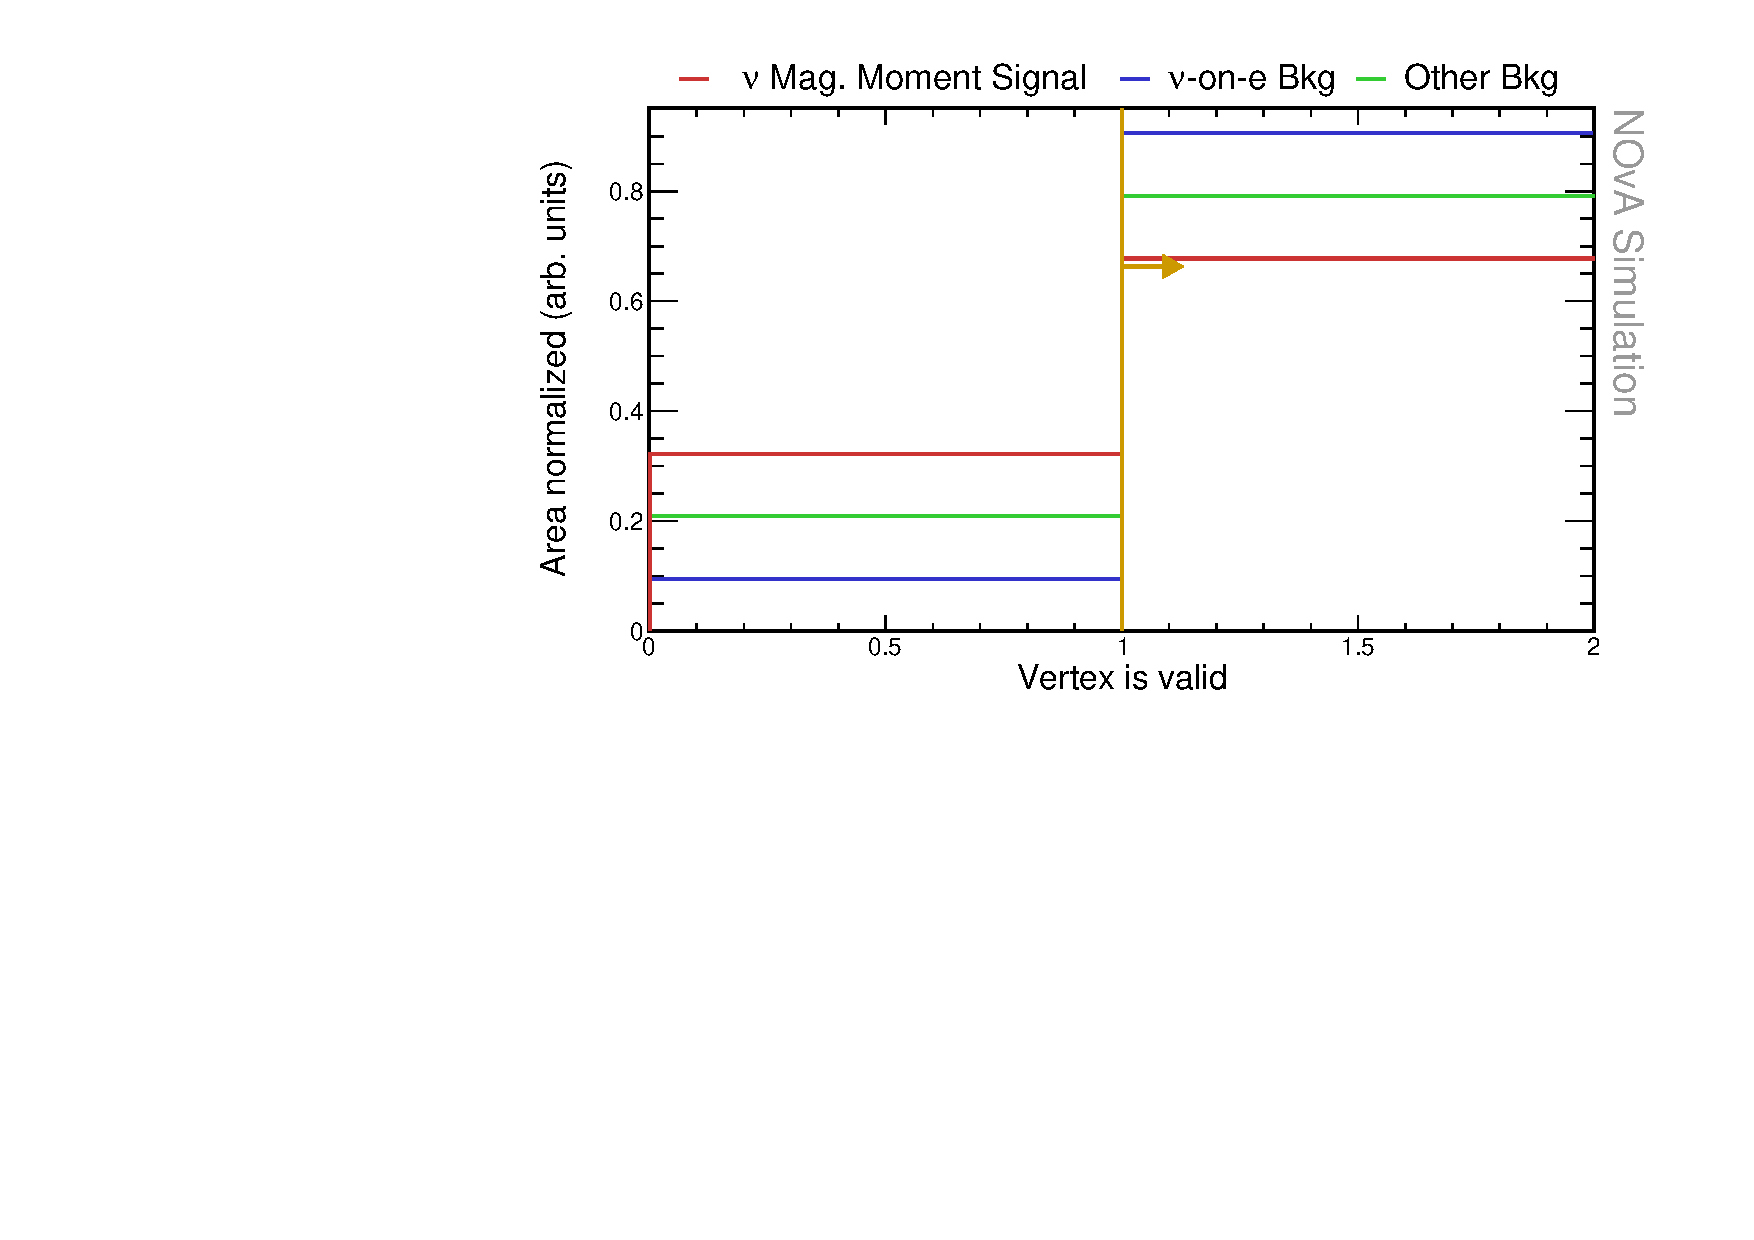
\includegraphics[width=.7\textwidth]{Plots/NuMMEventSelection/N1Cut_vtxIsValid.pdf}
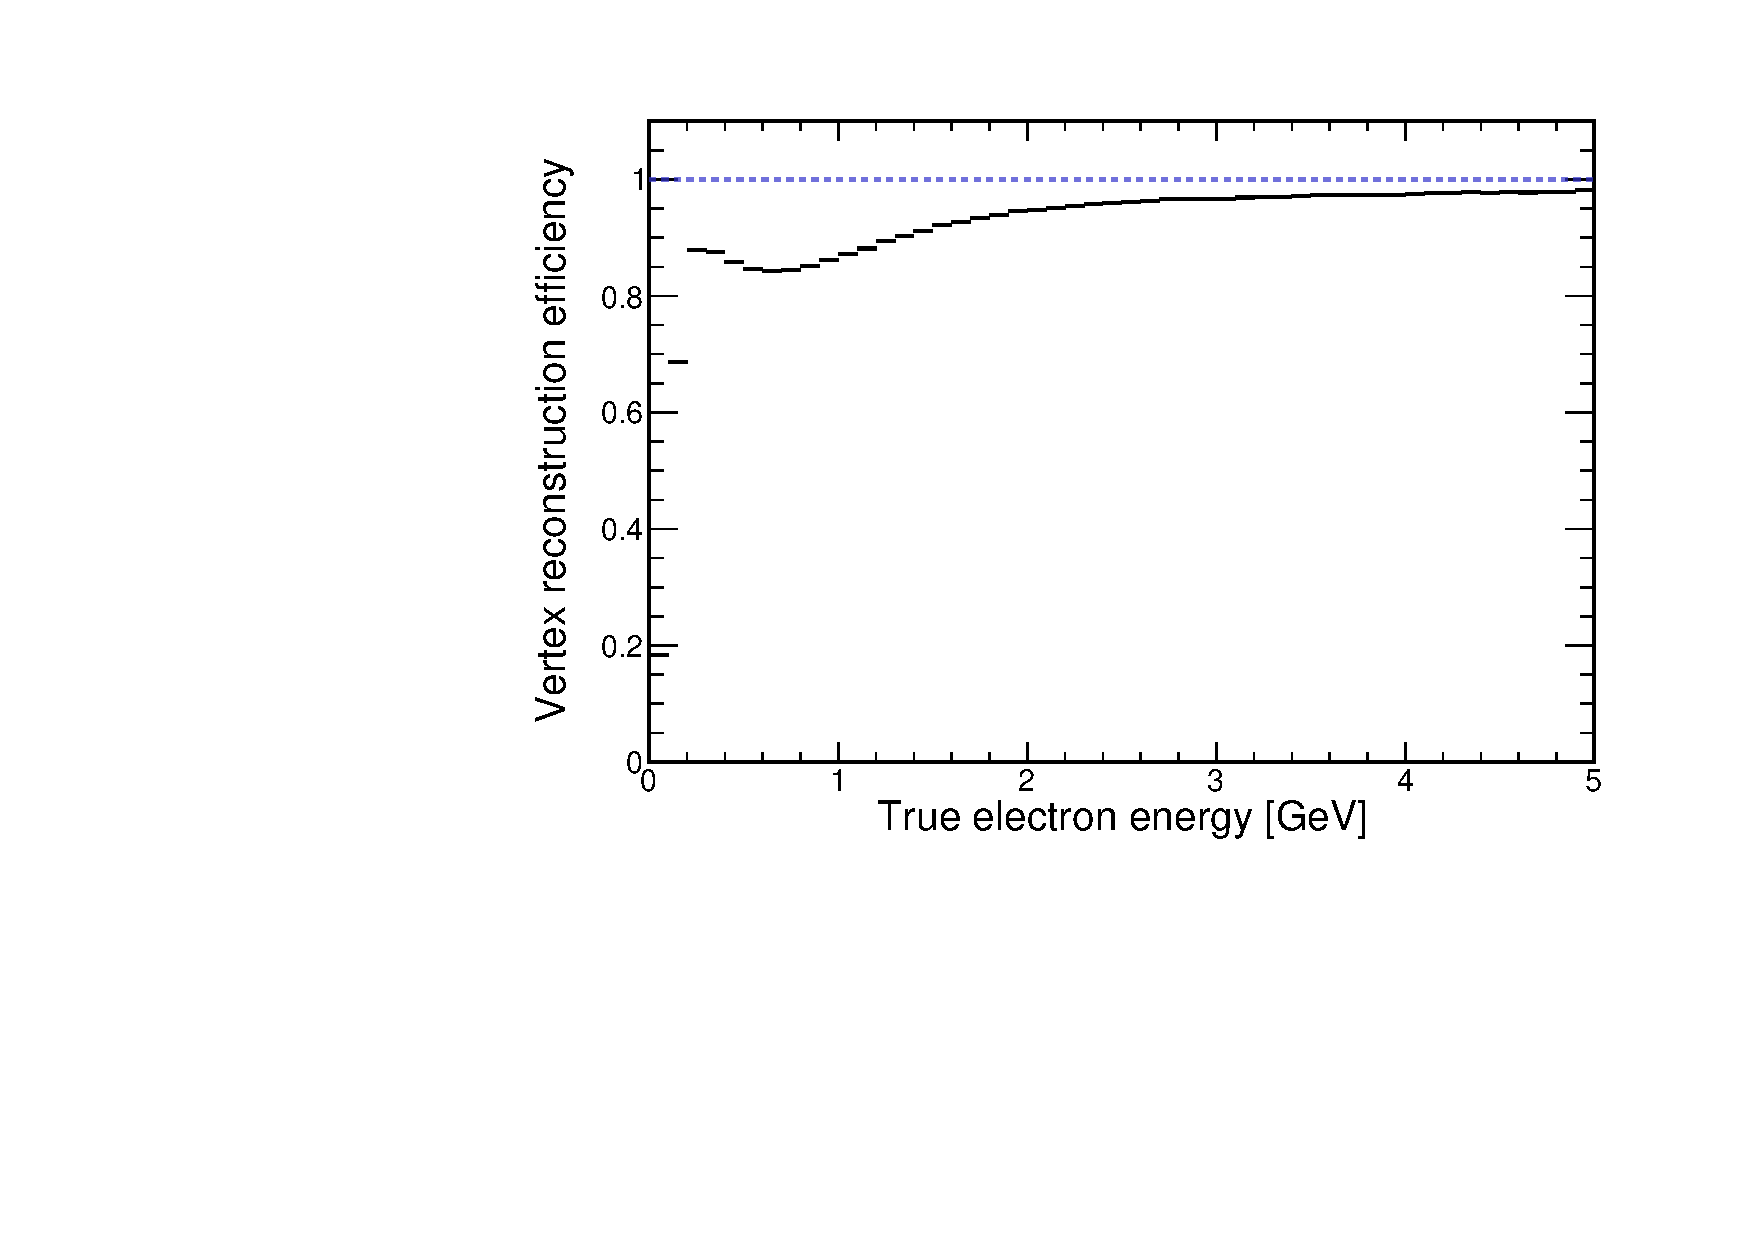
\includegraphics[width=.7\textwidth]{Plots/NuMMEventSelection/VtxIsValidNuMM.pdf}
\caption[Vertex reconstruction quality cut]{Top: Relative comparison of the signal (red), \acrshort{nuone} background (blue), and other background (green) events for the vertex reconstruction quality selection. Each histogram is area-normalised and the first bin corresponds to events without a valid vertex and second bin to events with correctly reconstructed vertex. The yellow line indicates the chosen cut value, where all events have to have a valid reconstructed vertex. Bottom: profile histogram of the `vertex is valid' variable as a function of the true electron energy for the true signal events, showing the significant drop in vertex reconstruction efficiency at low electron recoil energies. No selection was applied prior to making these plots.}
\label{fig:NuMMCutsVertexIsValid}
\end{figure}

Additionally, we limit the number of hits per plane to $<6$. This is to remove the so-called `\gls{FEB} flashers', which are caused by such a high energy deposit in one cell, that it affects all the other channels on the same \gls{APD} \cite{NOvA-doc-37668}. The cut value was chosen so that it removes approximately $\unit[0.25]{\%}$ signal events, which is the same criterion as is used for the pre-selection cuts described below. Relative comparisons between signal and background for the number of prongs and the number of hits per plane are shown in Fig.~\ref{fig:NuMMCutsRecoQuality}.

%In pre-selection we also include a cut on the time difference between the mean times of the "current" slice and of the slice closest in time, which should be $>25\ \unit{ns}$. This ensures that ... \todo{This is to remove slicing failures that split the two gamma from a $\pi^0$ into two slices that resemble electron signal. Should we remove them now though?}.

%[nueXSec ana, docdb:37668] One additional detector issues is the presence of "FEB Flashers" within reconstructed slices. FEB flashers are caused by high  energy deposits in one cell, which induces a sagged baseline in all other channels on the same APD. When the baseline is restored, fake hits are triggered on the whole APD.

\begin{figure}[hbtp]
\centering
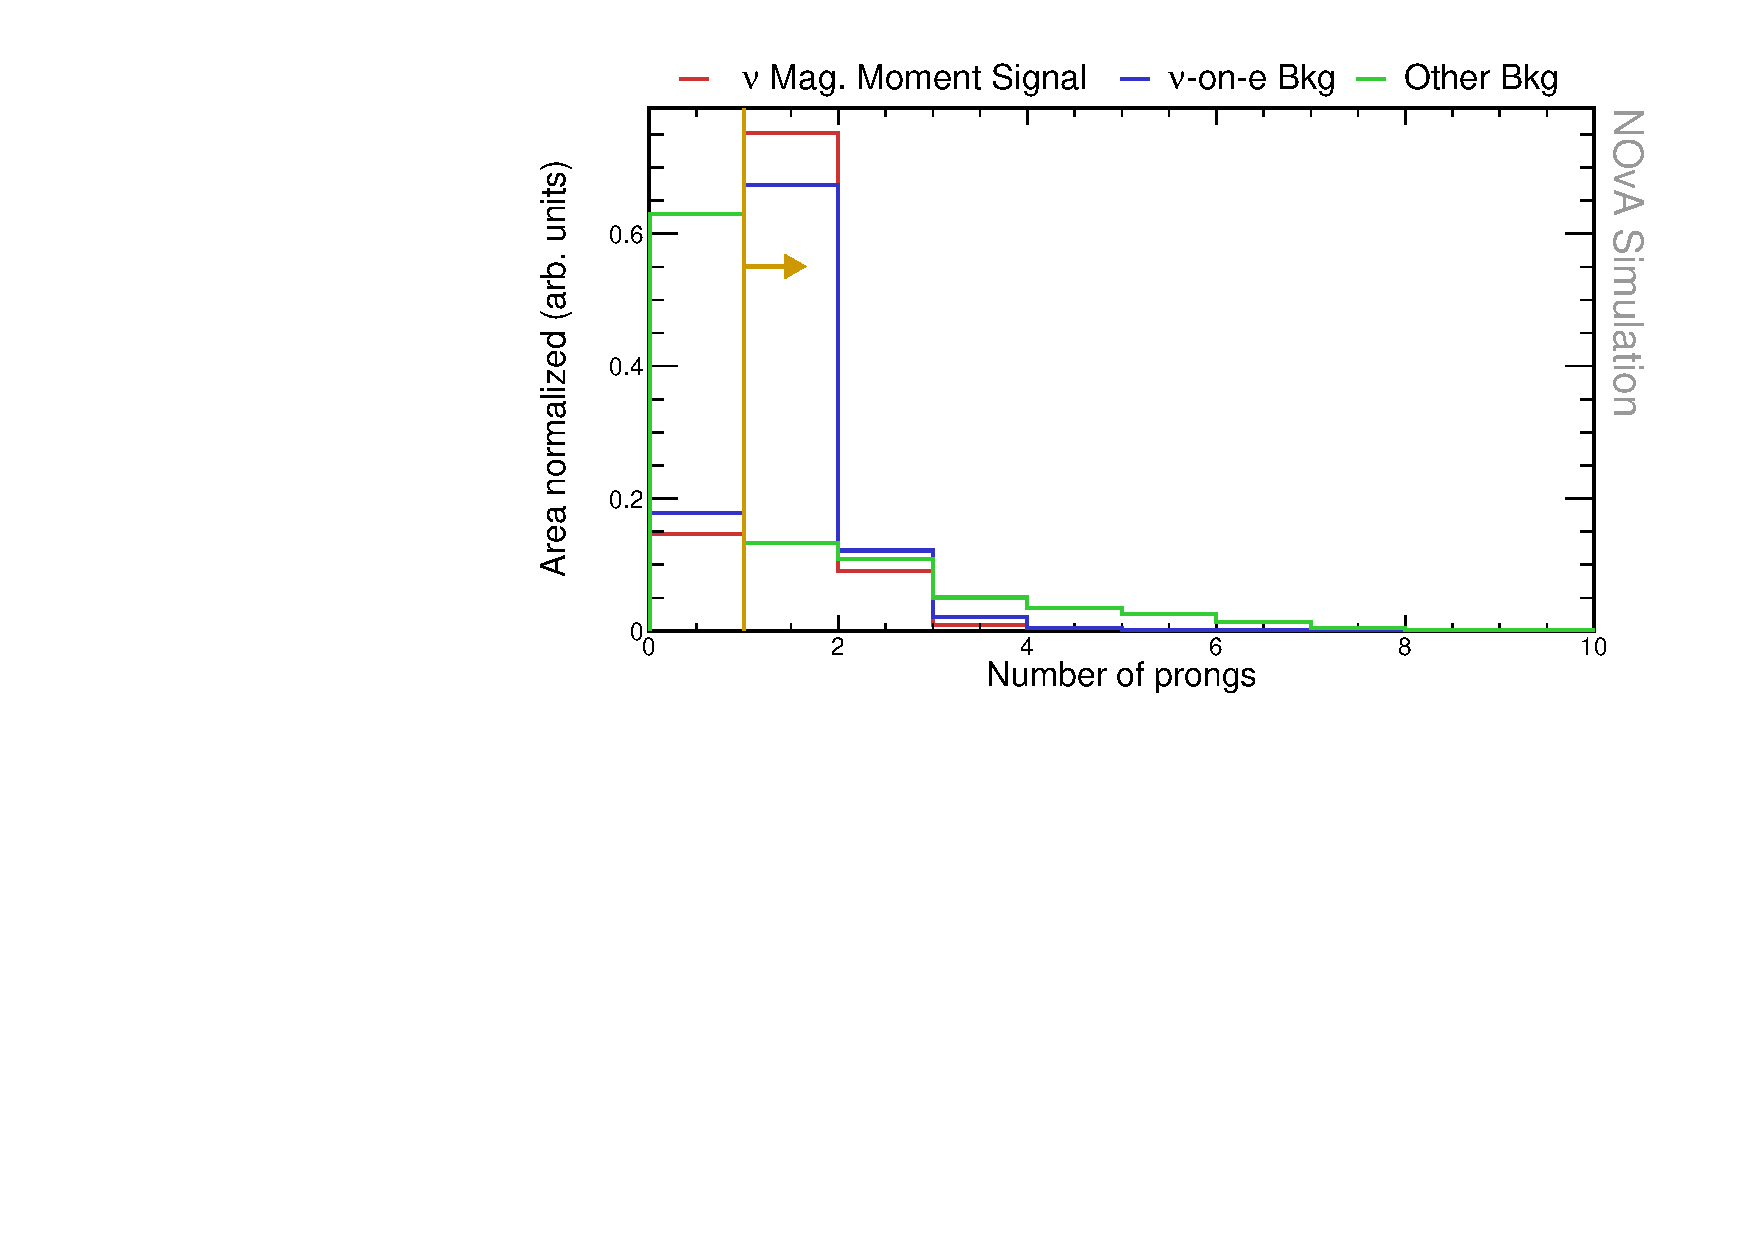
\includegraphics[width=.7\textwidth]{Plots/NuMMEventSelection/N1Cut_NPng.pdf}
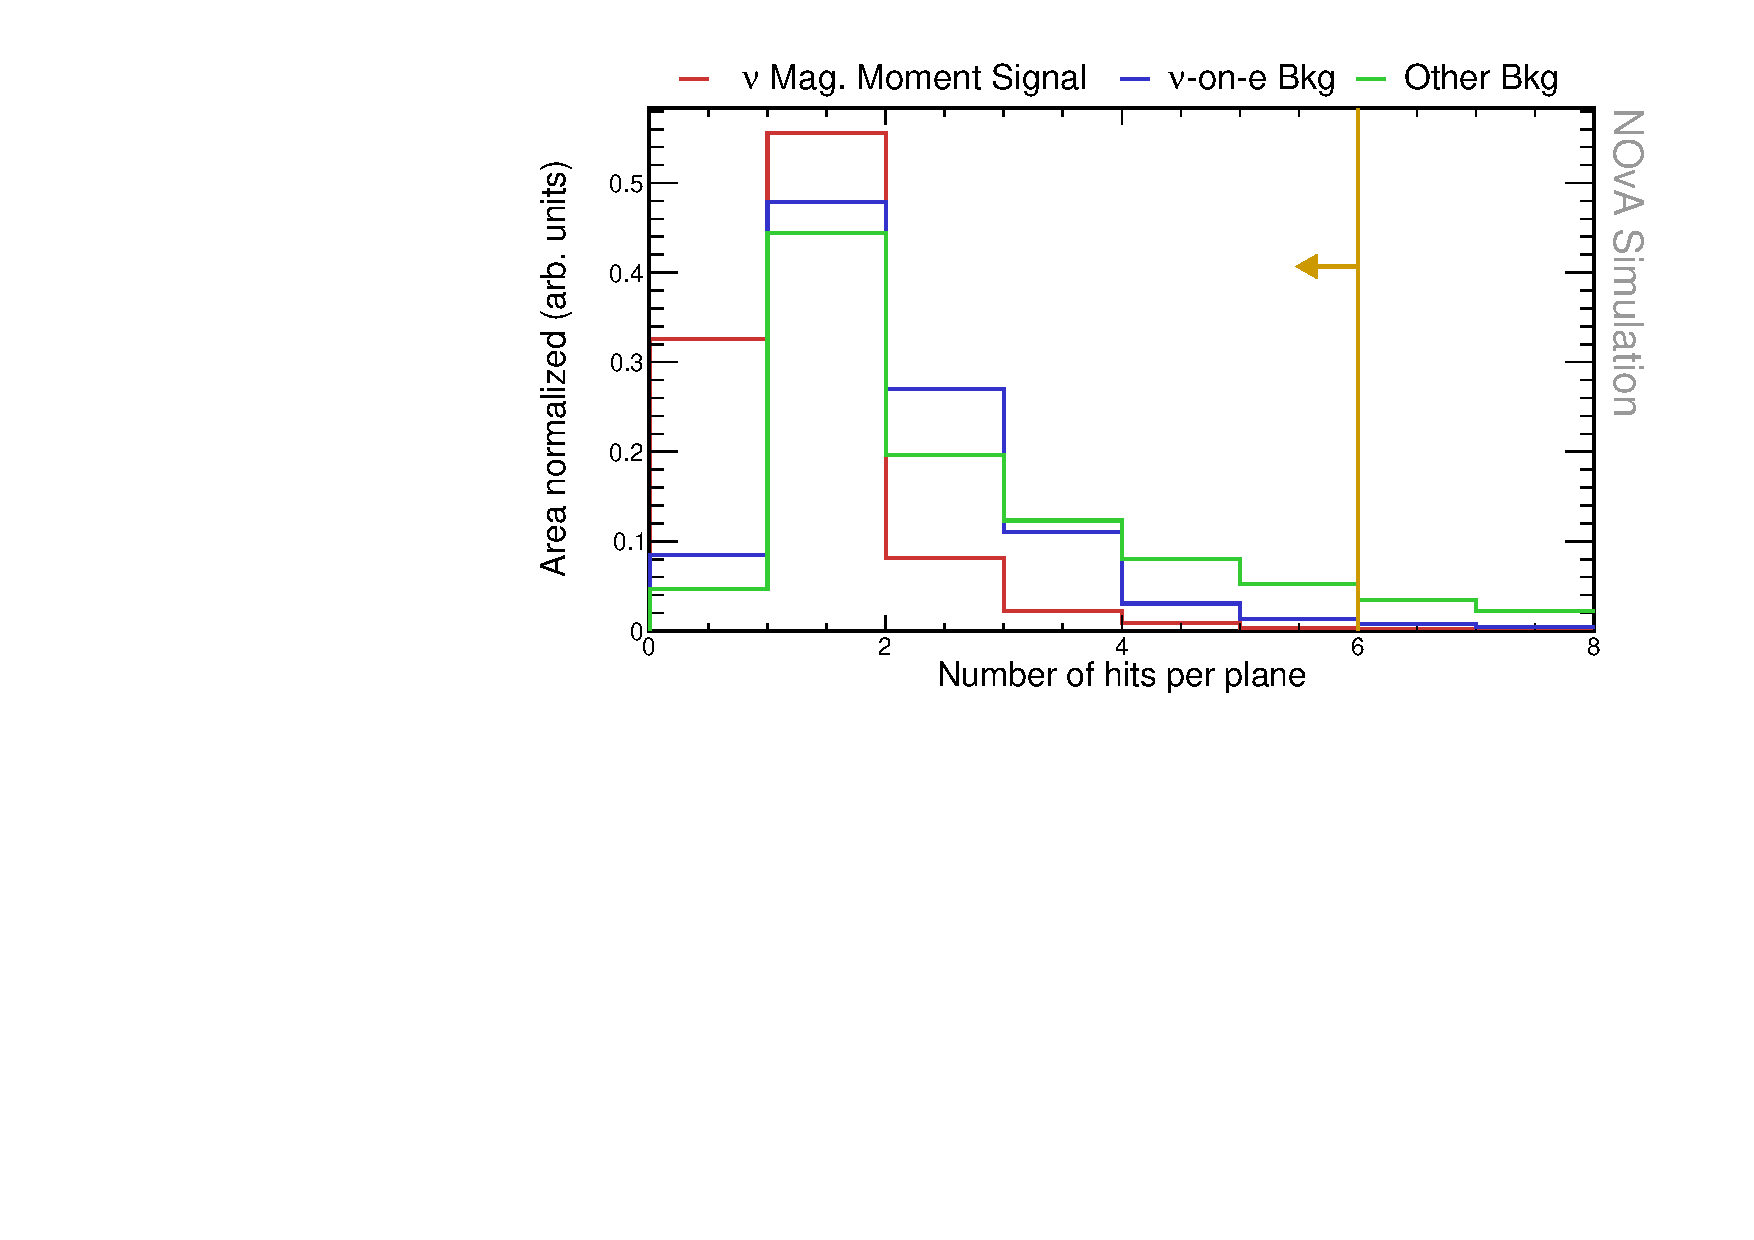
\includegraphics[width=.7\textwidth]{Plots/NuMMEventSelection/N1Cut_NHitsPPlane.pdf}
\caption[Prong and hits reconstruction quality cuts]{Relative comparison of signal (red), \acrshort{nuone} background (blue), and other background (green) events in the number of prongs (top) and the number of hits per plane (bottom) distributions. Events in both plots are required to have a valid reconstructed vertex and in the bottom plot also at least one reconstructed prong. Yellow lines indicate the cut values for the shown variables, with arrows pointing towards the preserved events. All histograms are area-normalised.}
\label{fig:NuMMCutsRecoQuality}
\end{figure}

%%% Low CalE
Furthermore, the reconstructed calorimetric energy of the primary shower is required to be $E_{cal} > \unit[0.5]{GeV}$ as shown in Fig.~\ref{fig:NuMMCutsLowCalE}. This is primarily due to the limitations of the currently used \gls{CVN}-based \gls{nuone} identifiers described in Sec.~\ref{sec:NuMMEventSelTMVA}, which were developed and validated for \gls{nuone} events with energies above this limit, to avoid the large background at low energies. However, due to the nature of the neutrino magnetic moment signal, which is concentrated at low electron recoil energies, this cut also removes a majority of our signal events, specifically $\unit[66.8]{\%}$. This large reduction severely impacts the significance of our measurement. On the other hand, it also marks potentially the most impactful improvement available in a future re-analysis. There are other event identifying algorithms available in \gls{NOvA} that could be explored for \gls{nuone} events to leverage the low energy sample. Additionally, it is possible to develop a purpose-built \gls{nuone} identifier focusing on low electron recoil energies.

\begin{figure}[hbtp]
\centering
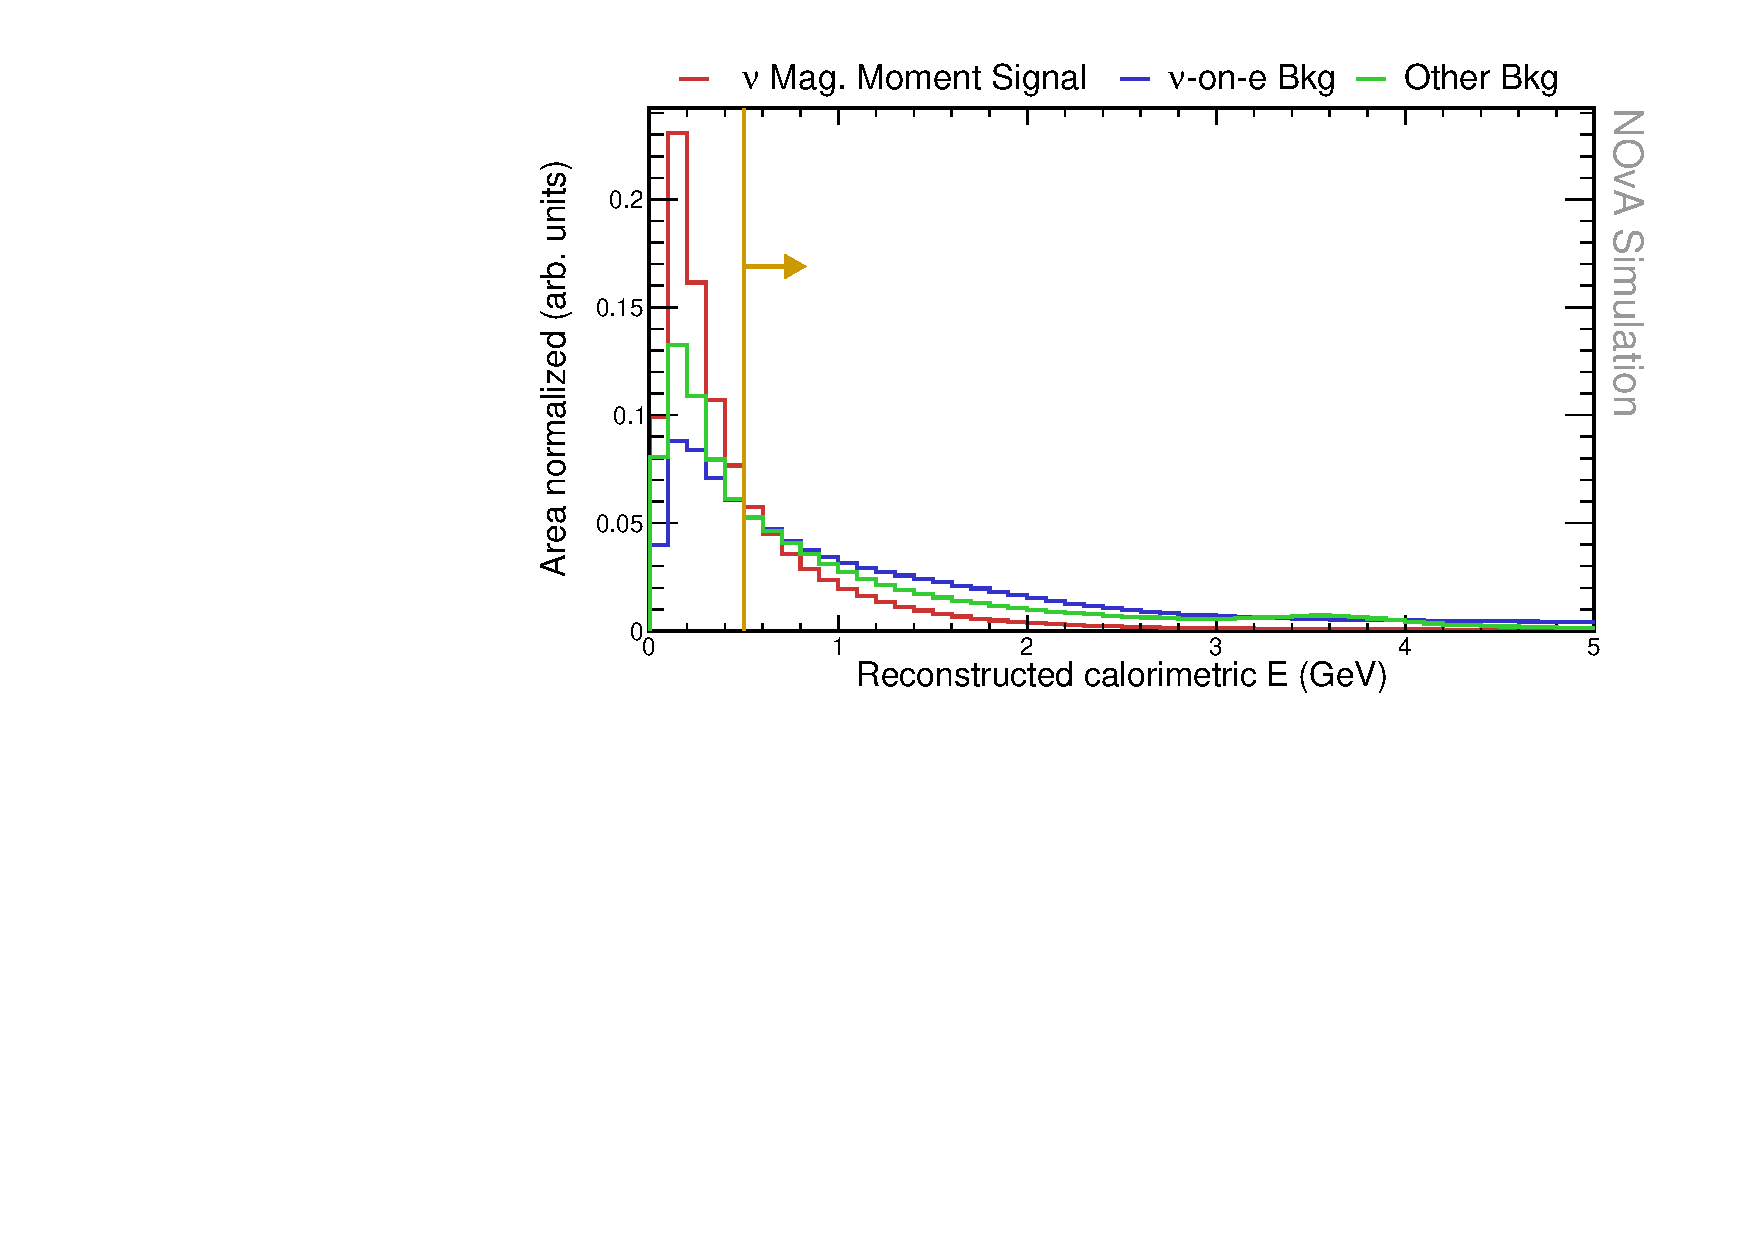
\includegraphics[width=.7\textwidth]{Plots/NuMMEventSelection/N1Cut_calELow.pdf}
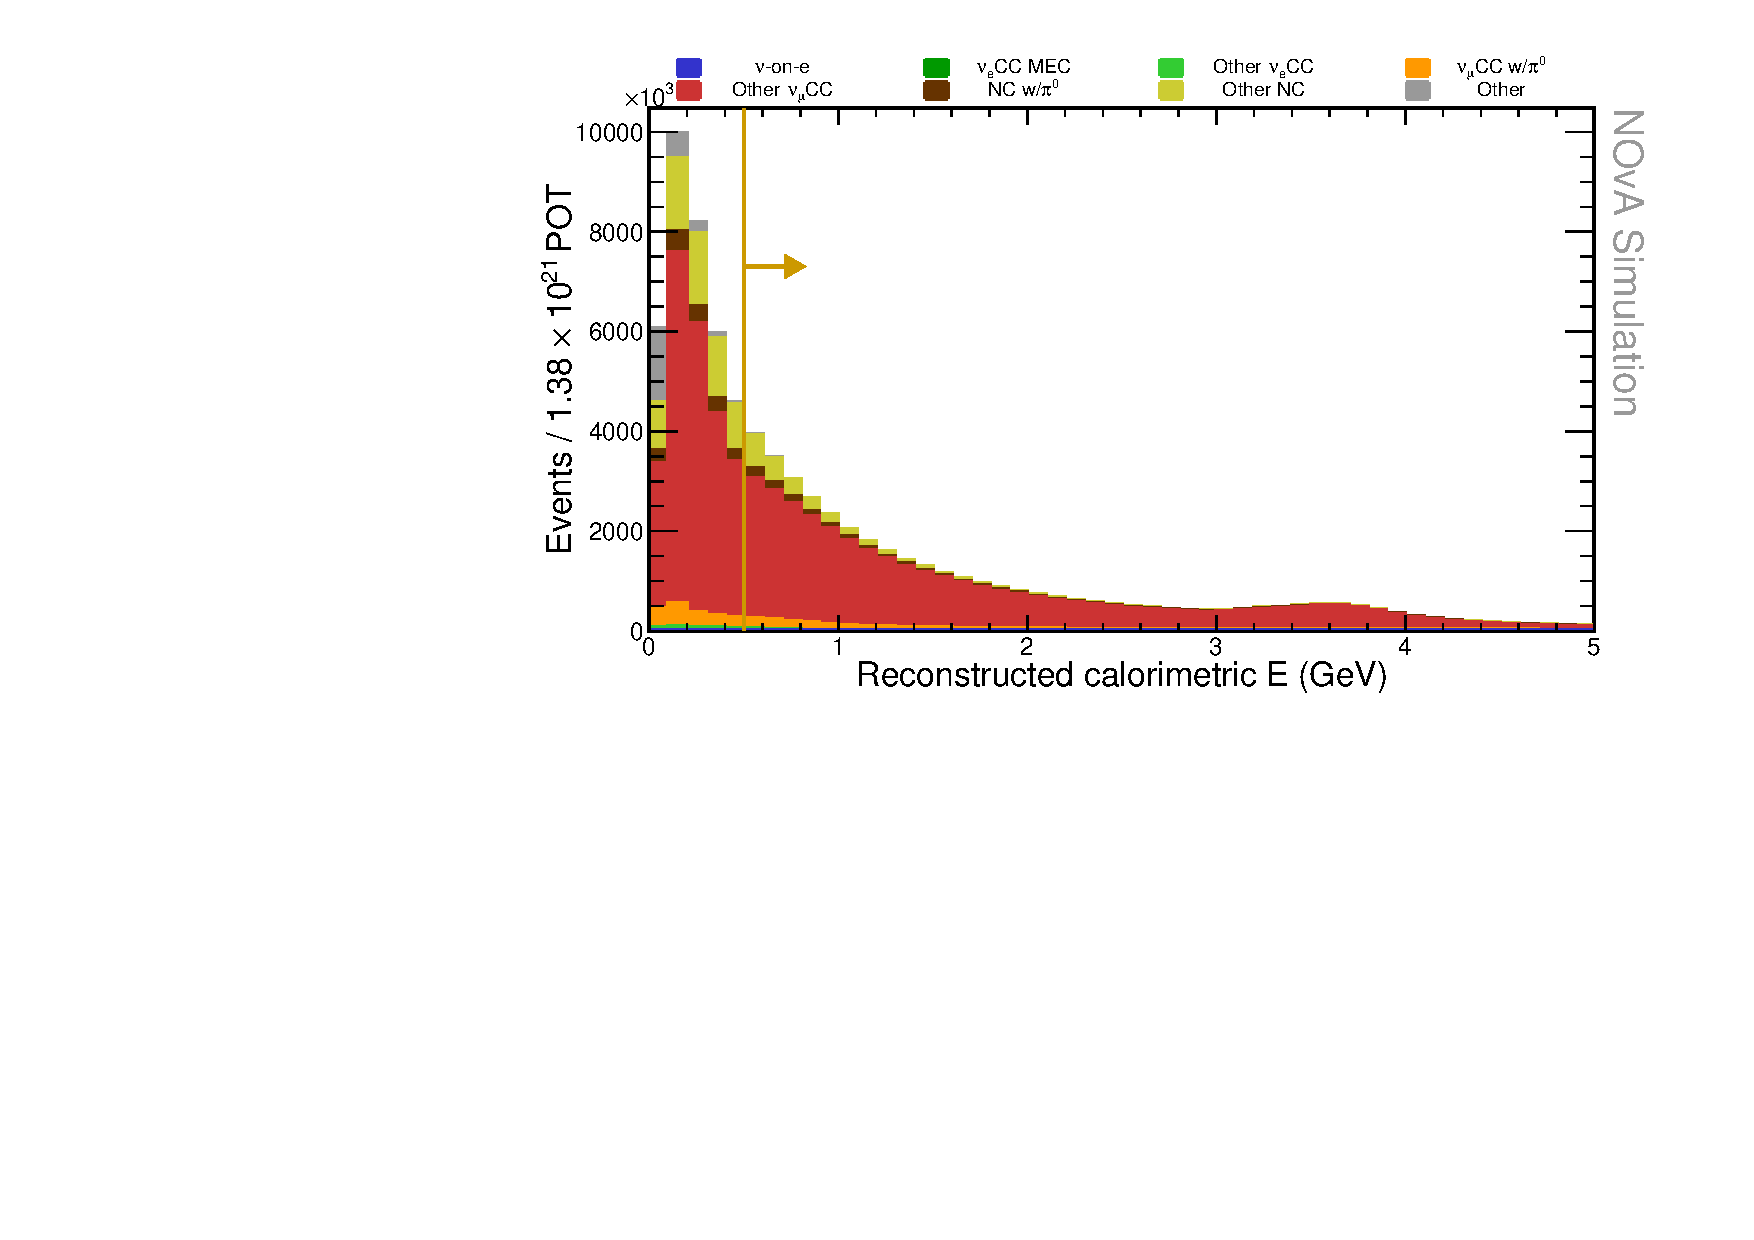
\includegraphics[width=.7\textwidth]{Plots/NuMMEventSelection/N1Cut_calELow_BkgDecomp.pdf}
\caption[Low calorimetric energy cut for reconstruction quality]{Top: Relative comparison of signal (red), \acrshort{nuone} background (blue), and other background (green) events in the reconstructed calorimetric energy distribution. All histograms are area-normalised. Bottom: Decomposition of background into various sub-samples, normalised to the data \acrshort{POT} exposure. Events in both plots are required to have a valid reconstructed vertex, at least one reconstructed prong and less than $6$ hits per plane. Yellow lines indicate the cut value for the reconstructed calorimetric energy, with arrows pointing towards the preserved events.}
\label{fig:NuMMCutsLowCalE}
\end{figure}

\begin{table}[!hb]
\centering
\caption[Event selection cutflow table for the reconstruction quality cuts]{Event selection cutflow table for the reconstruction quality cuts showing the number of events and the relative efficiency of each cut for each signal sample. The relative efficiency is calculated as number of events remaining after applying the corresponding cut divided by number of events for all the previous cuts. All the cuts are listed in sequence as they are applied.}
\begin{tabular}{|l|cc|cc|cc|}\hline
\multicolumn{1}{|c|}{} & \multicolumn{2}{c|}{\textbf{Signal}} & \multicolumn{2}{c|}{\textbf{$\nu$-on-e bkg}} & \multicolumn{2}{c|}{\textbf{Other bkg}} \\
\multicolumn{1}{|c|}{\multirow{-2}{*}{\textbf{Selection}}} & \textbf{$N_{evt}$} & \textbf{$\epsilon_{rel}\left(\%\right)$} & \textbf{$N_{evt}$} & \textbf{$\epsilon_{rel}\left(\%\right)$}  & \textbf{$N_{evt}$} & \textbf{$\epsilon_{rel}\left(\%\right)$}\\\hline
\textbf{No Cut} & 817.34 & 100 & 6.82$\times 10^3$ & 100 & 2.96$\times 10^8$ & 100\\
\textbf{Valid Vtx} & 553.86 & 67.76 & 6.17$\times 10^3$ & 90.55 & 2.34$\times 10^8$ & 79.10\\
\textbf{N$^o$ Prongs} & 472.90 & 85.38 & 5.08$\times 10^3$ & 82.25 & 8.66$\times 10^7$ & 37.00\\
\textbf{Hits / Plane} & 471.14 & 99.63 & 4.97$\times 10^3$ & 97.85 & 7.32$\times 10^7$ & 89.56\\
\textbf{Low $E_{Shower}$} & 156.37 & 33.19 & 3.53$\times 10^3$ & 71.09 & 4.06$\times 10^7$ & 55.12\\\hline
\end{tabular}
\label{tab:CutflowTableBasicRecoQC}
\end{table}

\subsection{Pre-selection}\label{sec:NuMMEventSelectionPresel}
Pre-selection aims to remove obvious background events without significantly affecting the signal. The criterion we chose for the selection of these cuts is determined by the reduction of the signal efficiency by approximately $\unit[0.25]{\%}$ with each cut. This results in the total pre-selection reduction of the signal efficiency by approximately $\unit[1]{\%}$.

The first two variables used for our pre-selection are the same as were used in the event selection for the $\nu_e$ appearance \gls{ND} constraint for the three flavour neutrino oscillation measurements \cite{NOvAResults2021.pdf}. As we are searching for single electron showers, we can reduce backgrounds with multiple final state particles by limiting the total activity in the detector. Specifically, we require that the total number of hits assigned to all the reconstructed prongs is $<280$. This is shown in Fig.~\ref{fig:NuMMCutsNHitsLoose}. In general, the main background in \gls{NOvA} consists of the $\nu_\mu$\gls{CC} interactions, which are characterised by long muon tracks. We therefore limit the length of the longest reconstructed prong to be $<\unit[640]{cm}$, as shown in Fig.~\ref{fig:NuMMCutsLongestProng}. 

\begin{figure}[hbtp]
\centering
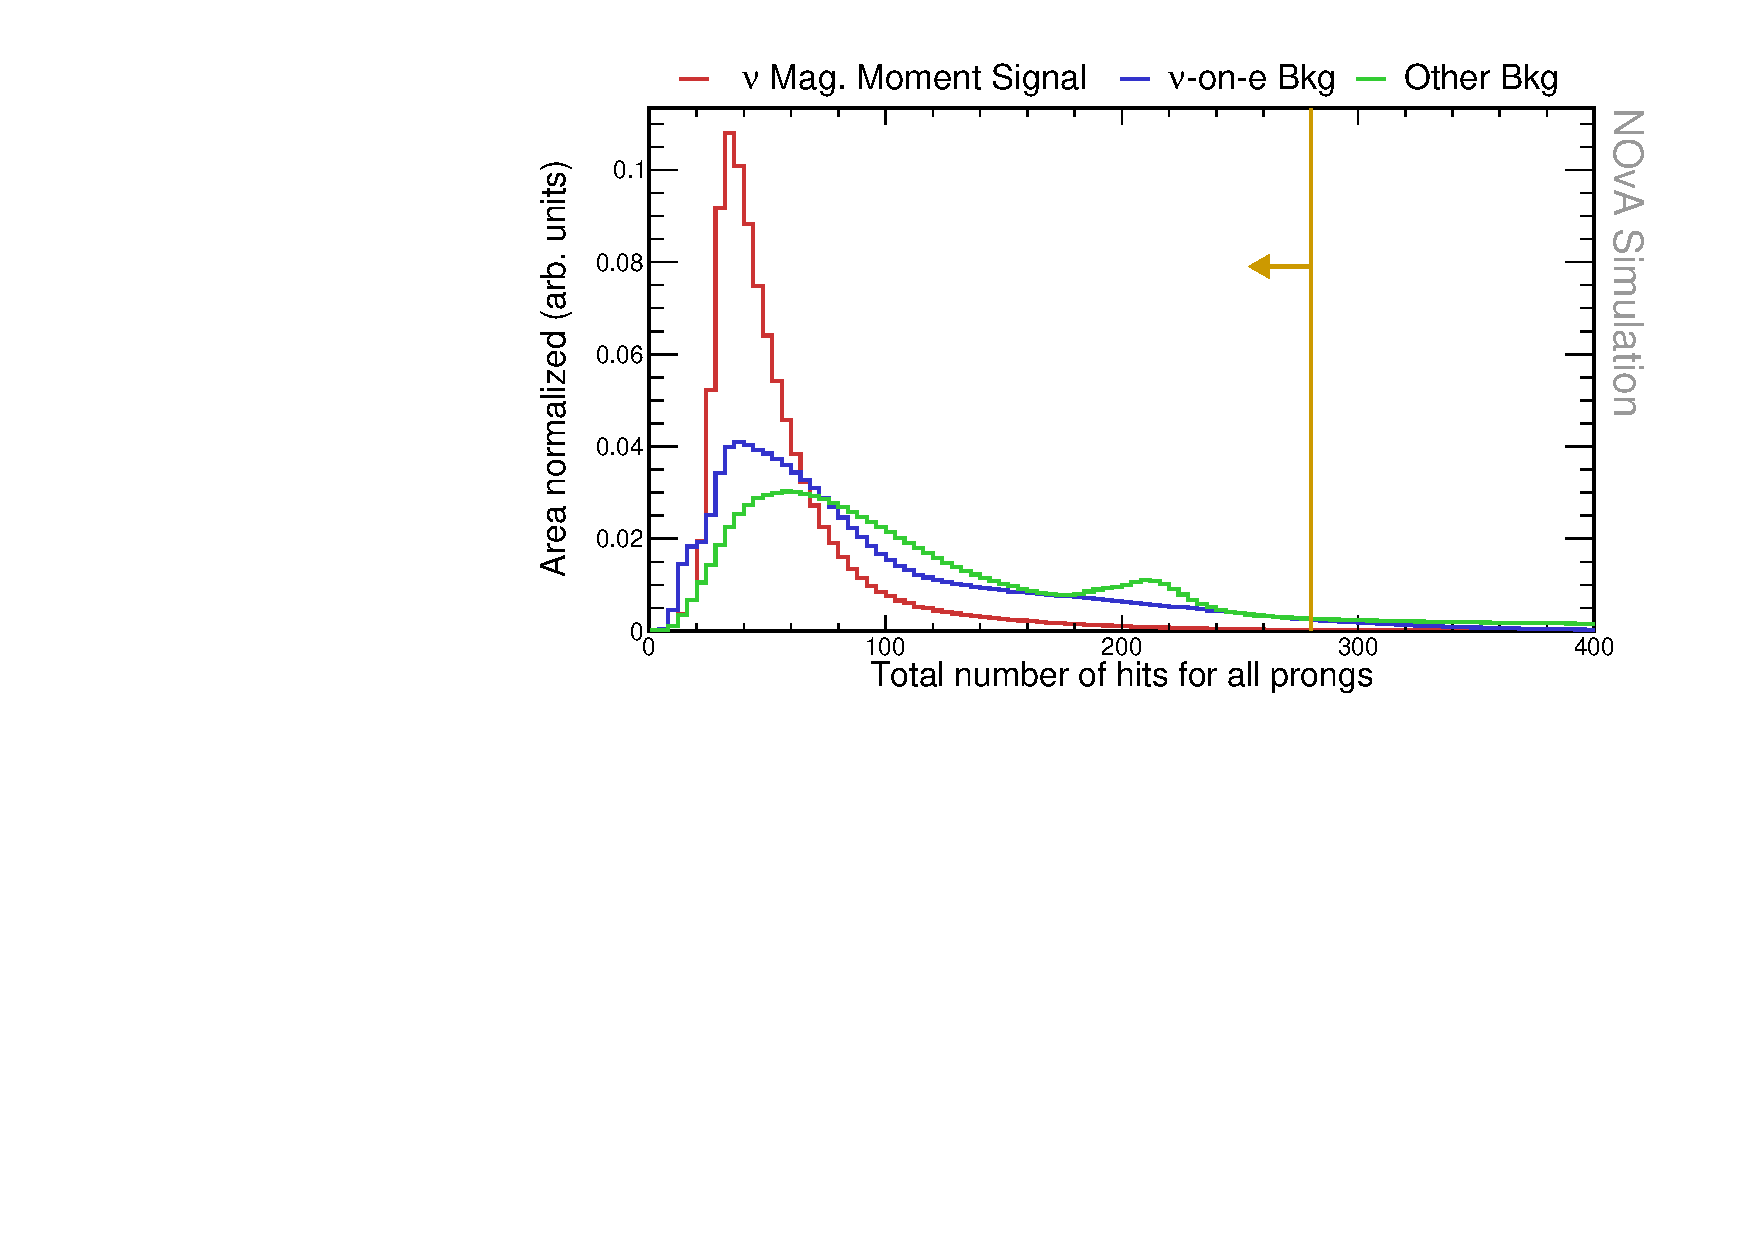
\includegraphics[width=.7\textwidth]{Plots/NuMMEventSelection/N1Cut_NHitsLoose.pdf}
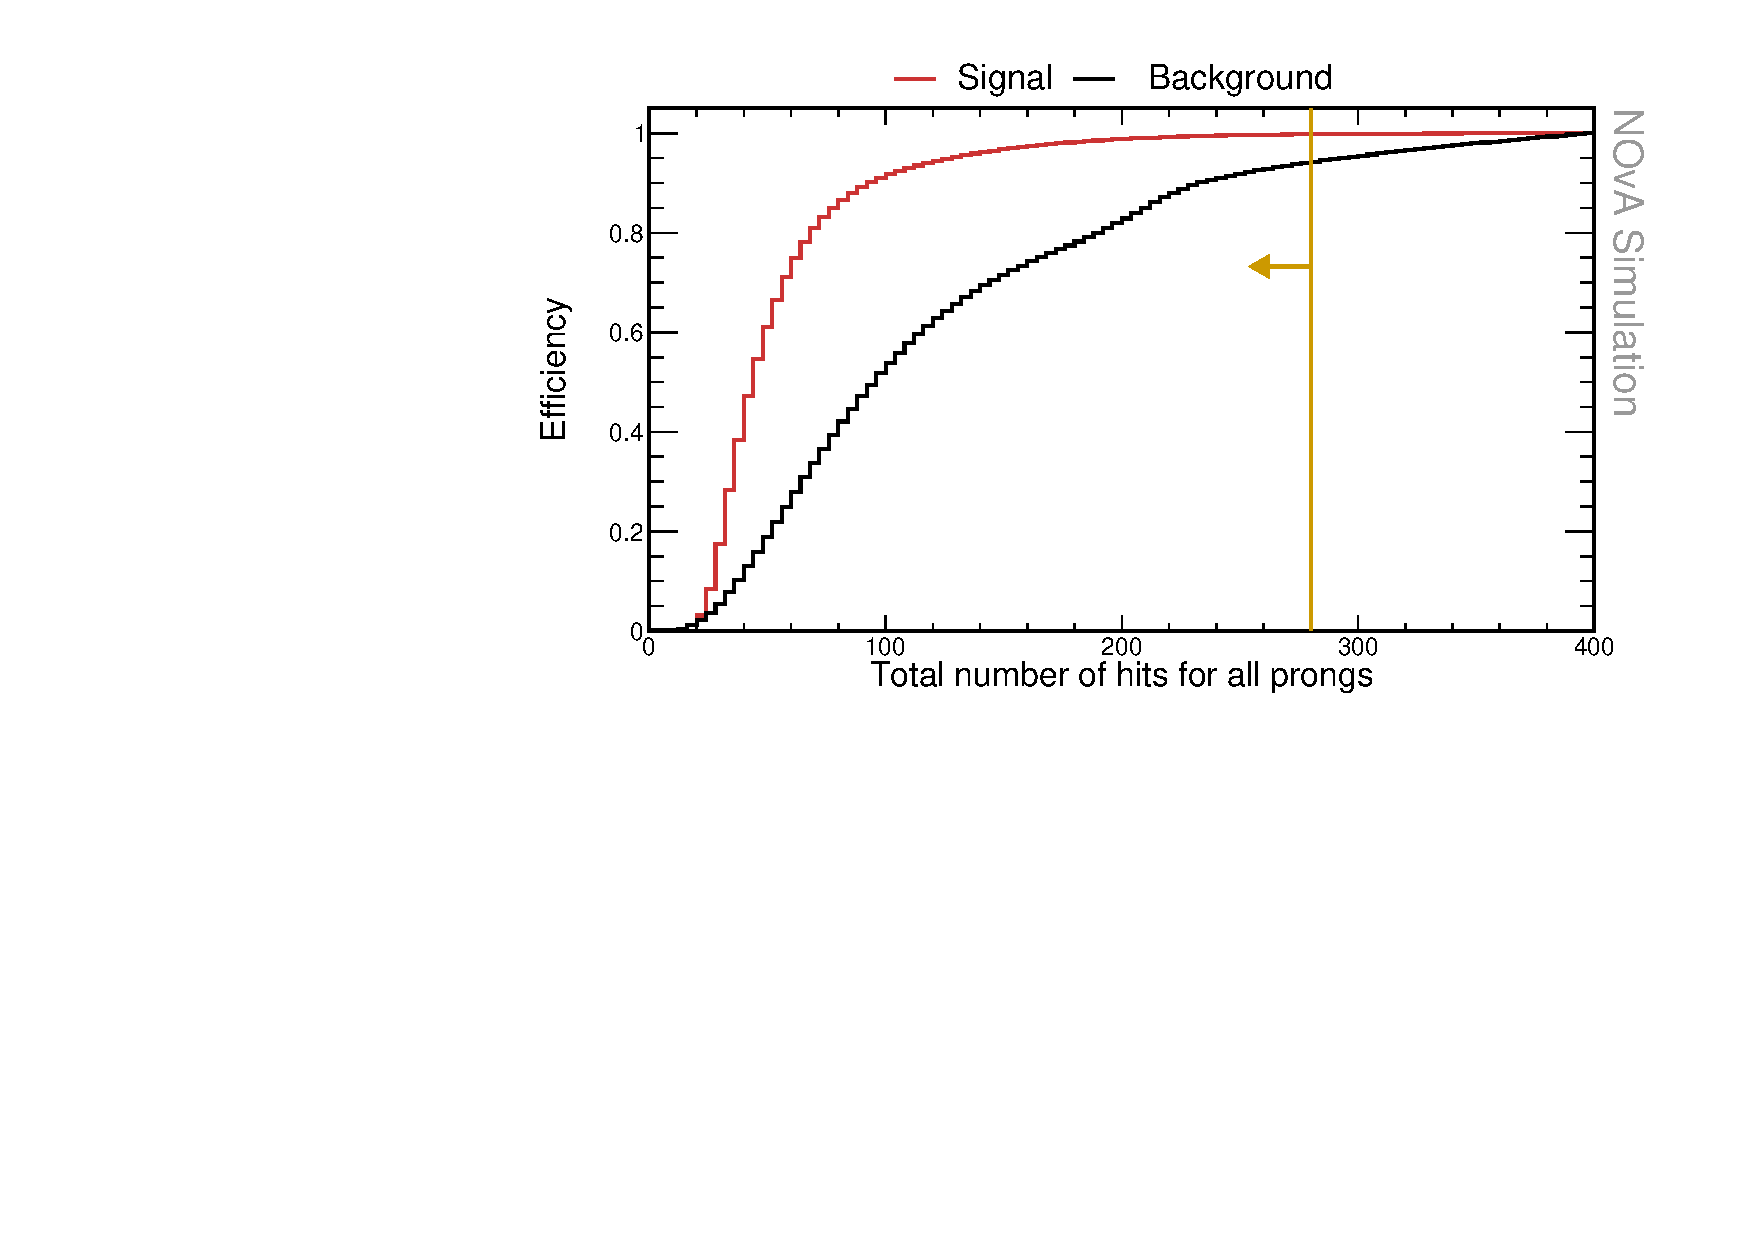
\includegraphics[width=.7\textwidth]{Plots/NuMMEventSelection/NuMM_N1Cut_NHitsLooseleft_Eff.pdf}
\caption[Number of hits cut for pre-selection]{Top: Relative comparison of signal (red), \acrshort{nuone} background (blue), and other background (green) events in the distribution of total number of hits from all reconstructed prongs in the slice. All histograms are area-normalised. Bottom: Cumulative signal (red) and background (black) efficiency calculated as number of signal/background events left of the bin divided by the total number of signal/background events. Yellow lines indicate the cut value for the maximum number of hits, with arrows pointing towards the preserved events. The reconstruction quality cuts were applied before making these plots.}
\label{fig:NuMMCutsNHitsLoose}
\end{figure}

\begin{figure}[hbtp]
\centering
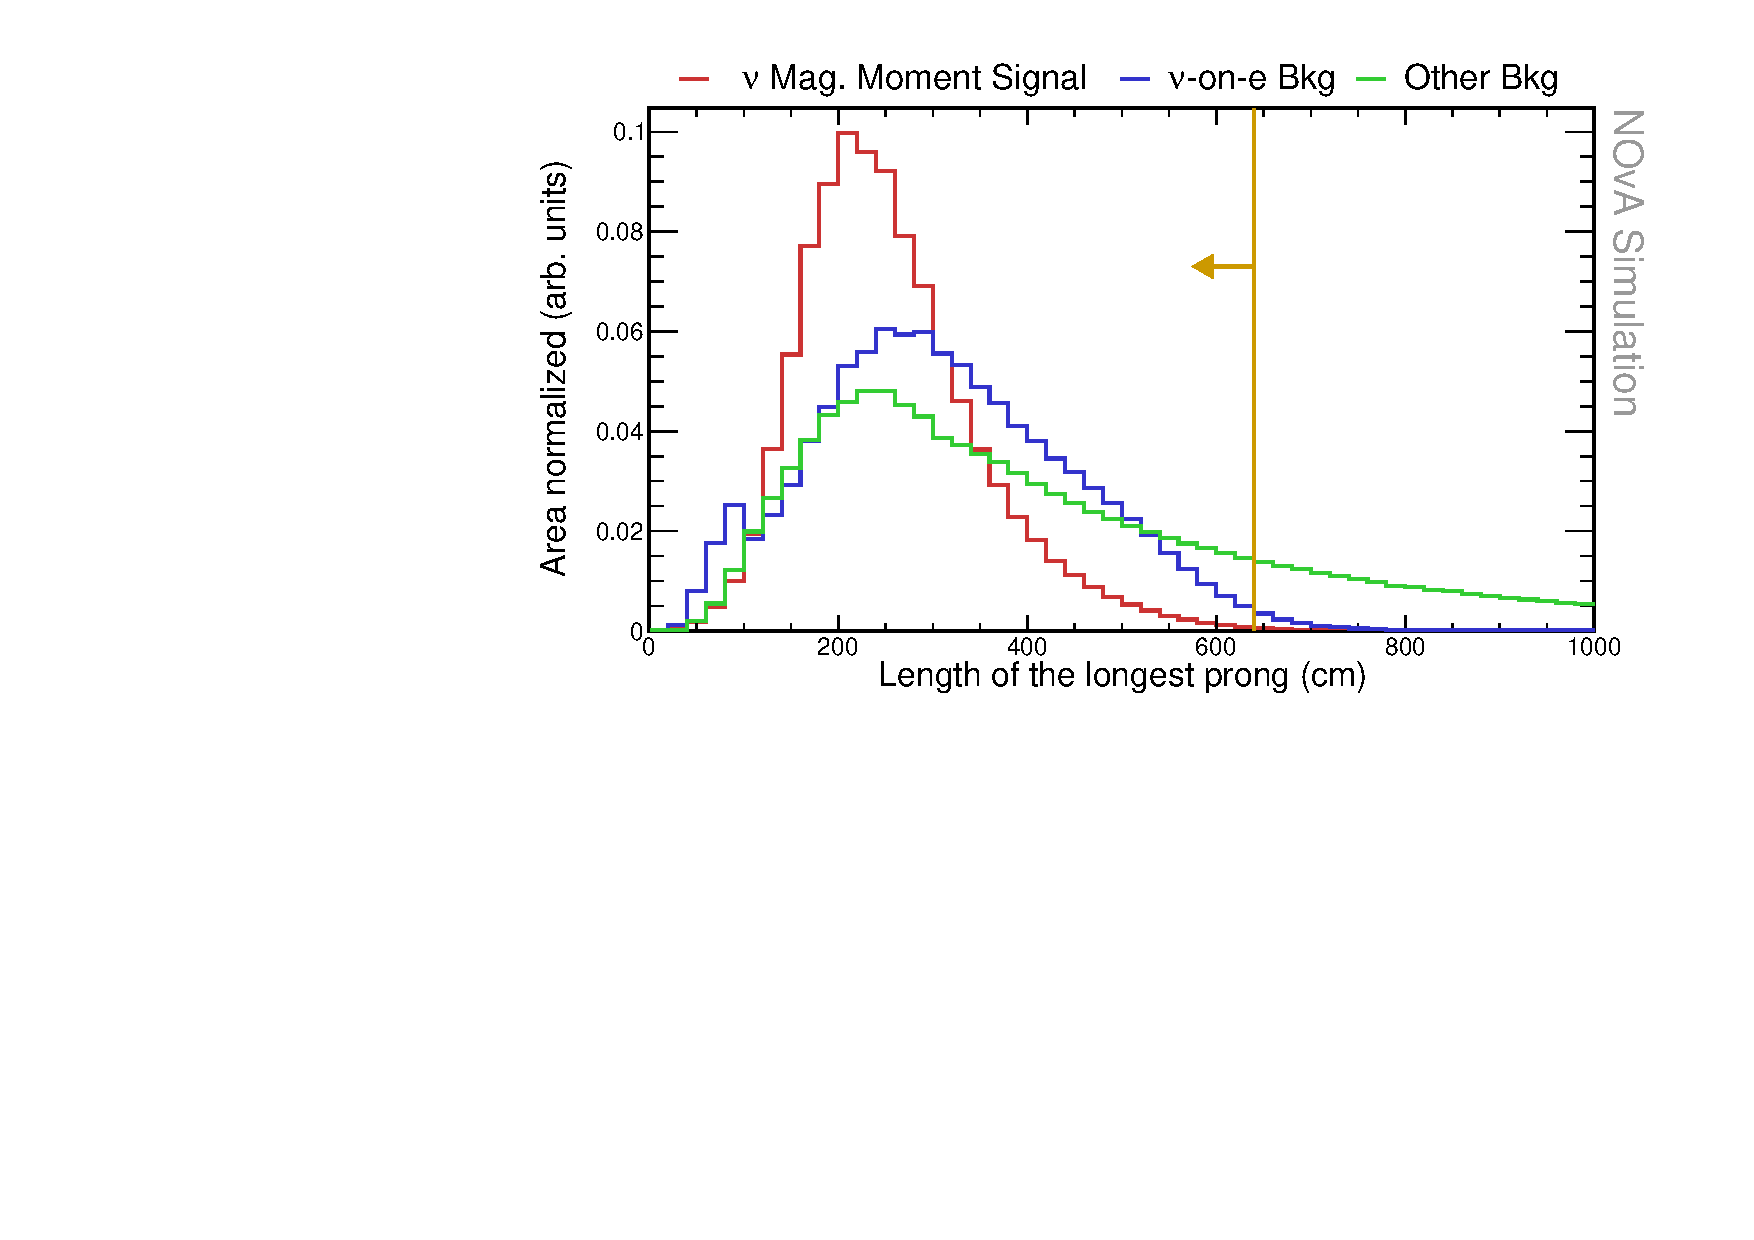
\includegraphics[width=.7\textwidth]{Plots/NuMMEventSelection/N1Cut_longestProng.pdf}
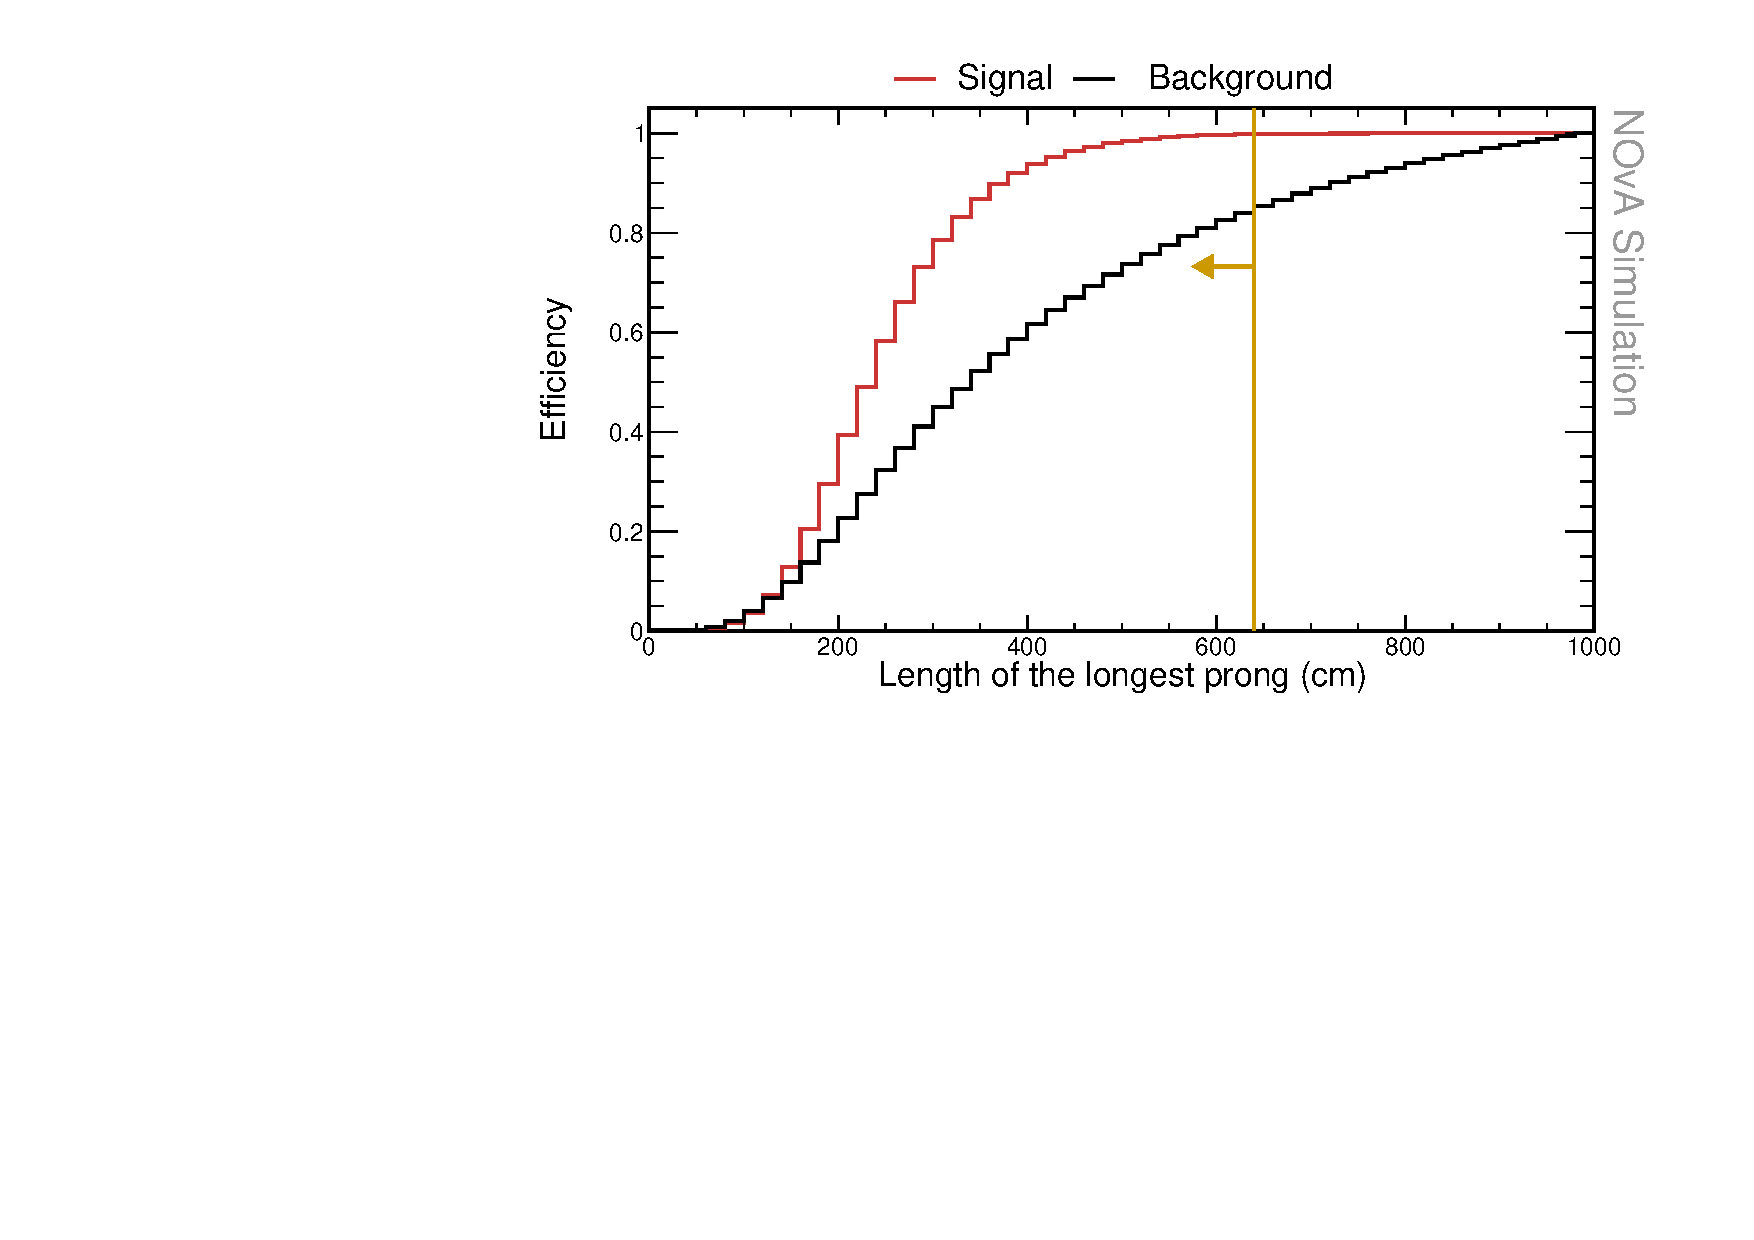
\includegraphics[width=.7\textwidth]{Plots/NuMMEventSelection/NuMM_N1Cut_longestProngleft_Eff.pdf}
\caption[Length of the longest prong cut for pre-selection]{Top: Relative comparison of signal (red), \acrshort{nuone} background (blue), and other background (green) events in the distribution of the length of the longest reconstructed prong in slice. All histograms are area-normalised. Bottom: Cumulative signal (red) and background (black) efficiency calculated as number of signal/background events left of the bin divided by the total number of signal/background events. Yellow lines indicate the cut value for the maximum length of the longest prong, with arrows pointing towards the preserved events. The reconstruction quality cuts and the number of hits cut were applied before making these plots.}
\label{fig:NuMMCutsLongestProng}
\end{figure}

Additionally, as discussed in Sec.~\ref{sec:MeasuringNuMM}, simple $2\rightarrow2$ kinematics dictate that the true electron recoil energy and angle for the \gls{nuone} interaction are limited by $E\theta^2<2m_e$. This can be used to distinguish \gls{nuone} elastic scattering from $\nu_e$\gls{CC} interactions, which also have an electron in the final state. However, due to unavoidable reconstruction deficiencies, the reconstructed $E\theta^2$ does not have such a strict cut-off value, and we are placing the pre-selection cut at $E\theta^2<0.064$, as can be seen in Fig.~\ref{fig:NuMMCutsETh2Loose}. Furthermore, some of the signal events can be reconstructed with the opposite direction with respect to the beam, which would result in $\theta\approx\unit[\pi]{rad}$. However, this reconstruction failure likely does not impact other reconstructed qualities and these events should be preserved for the final sample. For that reason, we are calculating the angle between the outgoing electron and the neutrino beam direction as $\arccos\left(\textsf{abs}\left(\cos\theta\right)\right)$, which gives the same value whether the shower is reconstructed forward or backwards.

\begin{figure}[hbtp]
\centering
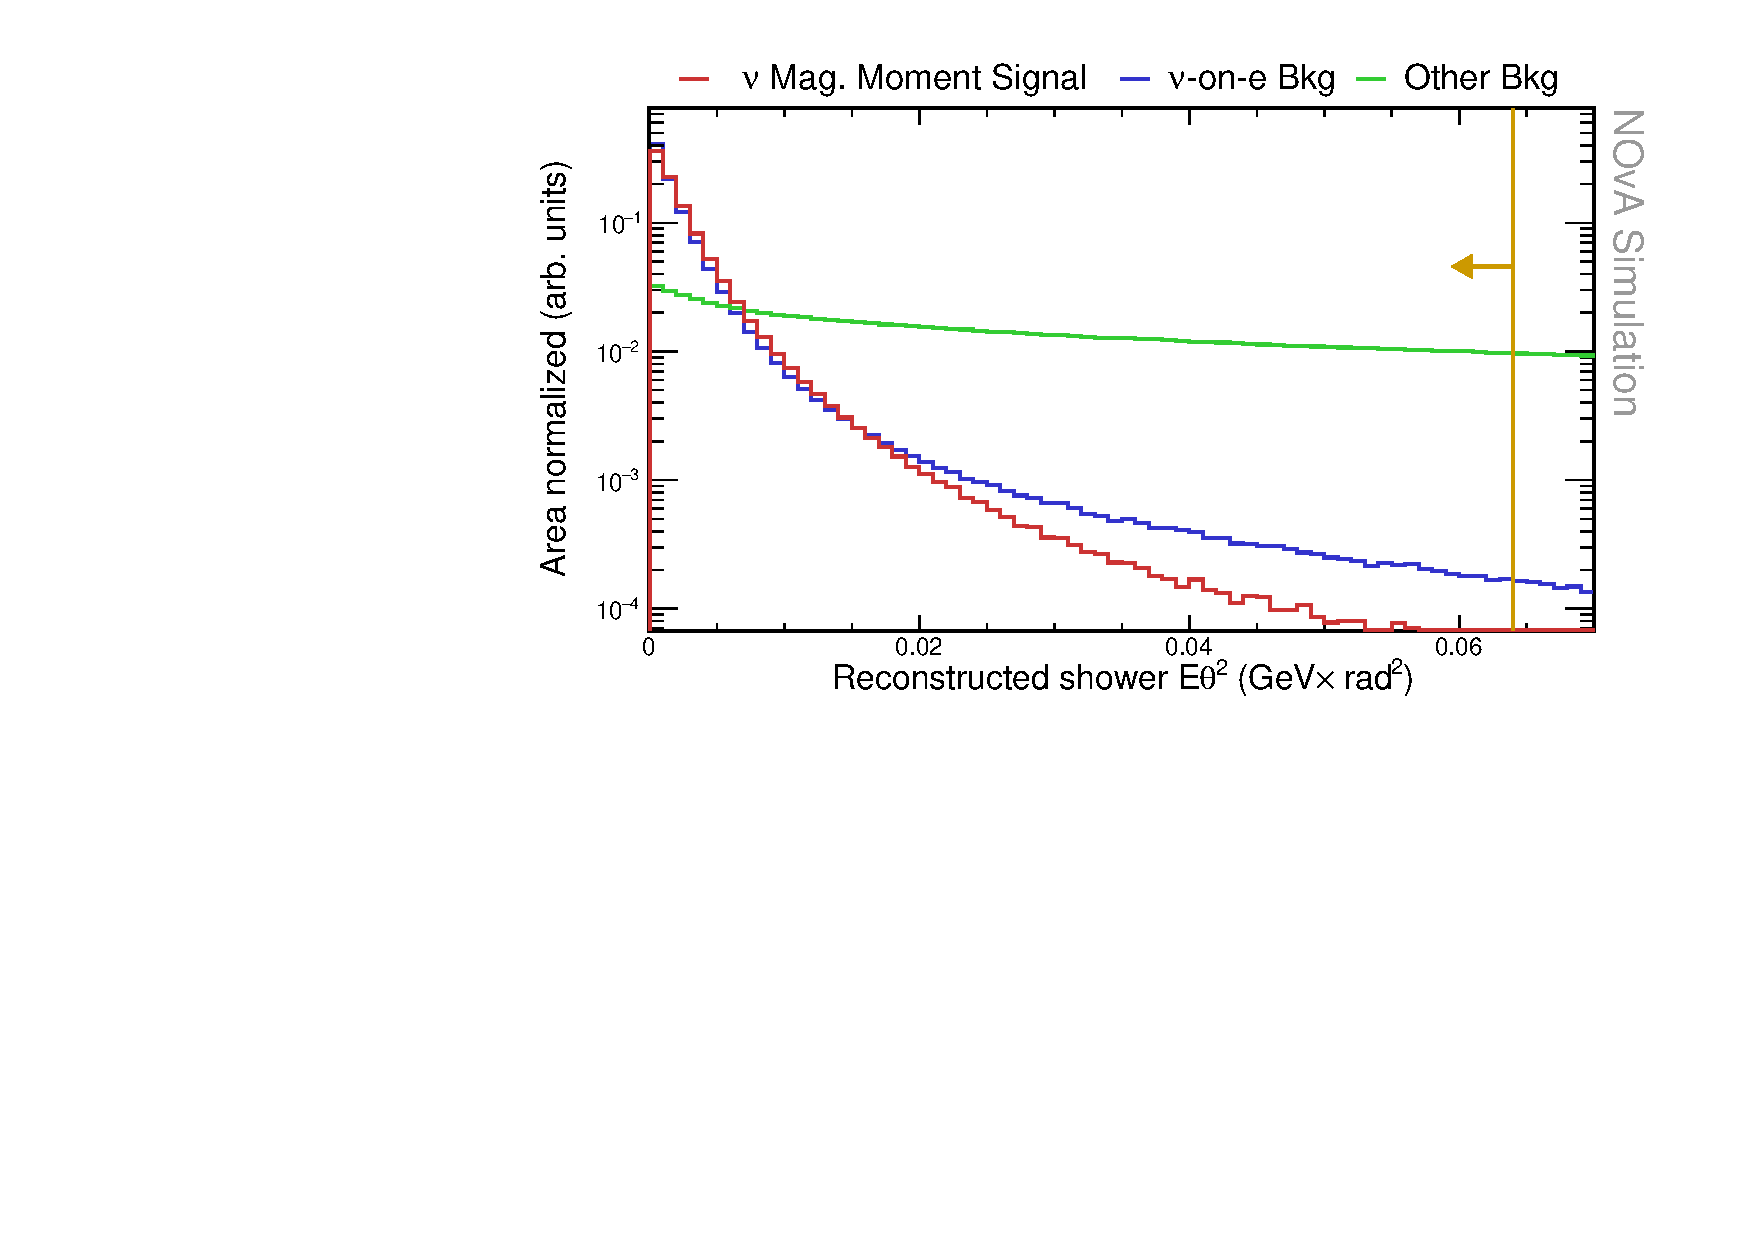
\includegraphics[width=.7\textwidth]{Plots/NuMMEventSelection/LogY_N1Cut_eth2Loose.pdf}
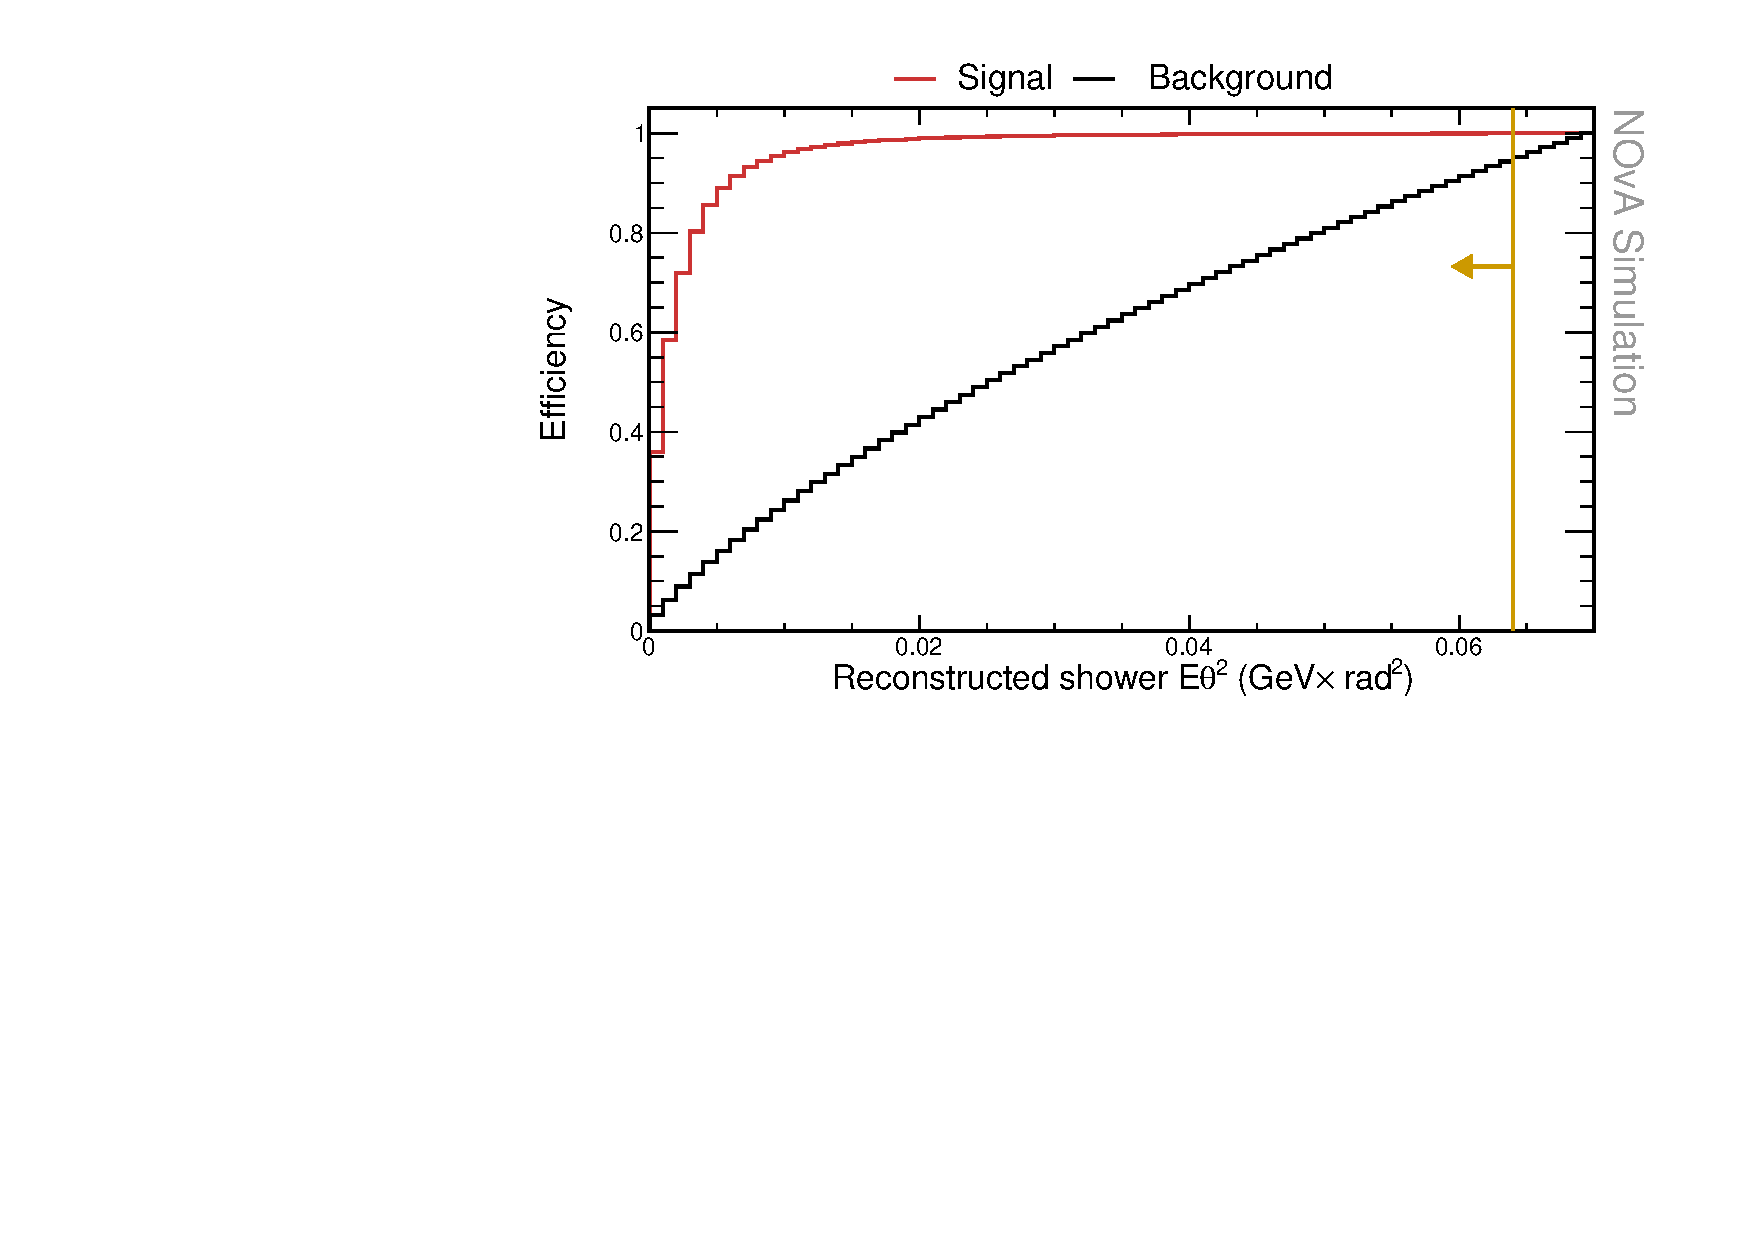
\includegraphics[width=.7\textwidth]{Plots/NuMMEventSelection/NuMM_N1Cut_eth2Looseleft_Eff.pdf}
\caption[$E\theta^2$ cut for pre-selection]{Top: Relative comparison of signal (red), \acrshort{nuone} background (blue), and other background (green) events in the distribution of the reconstructed energy of the leading shower multiplied by its angle from the incoming neutrino beam direction squared. All histograms are area-normalised with logarithmic y axis. Bottom: Cumulative signal (red) and background (black) efficiency calculated as number of signal/background events left of the bin divided by the total number of signal/background events. Yellow lines indicate the cut value for the depicted variable, with arrows pointing towards the preserved events. The reconstruction quality cuts, the number of hits cut, and the length of the longest prong cuts were applied before making both of these plots.}
\label{fig:NuMMCutsETh2Loose}
\end{figure}

The effect of the pre-selection cuts on the signal and background samples are summarised in Tab.~\ref{tab:CutflowTableBasicSelection}, where the first row lists the number of events after applying all the reconstruction quality cuts from Sec.~\ref{sec:NuMMEventSelRecoQC}. All three of the variables used for the pre-selection are employed again in the \gls{MVA}, as described in Sec.~\ref{sec:NuMMEventSelTMVA}.

%\todo{Add the DeCAF cuts description here - might describe them already when introducing the decaf samples, not sure yet}

\begin{table}[!hb]
\centering
\caption[Event selection cutflow table for the pre-selection]{Pre-selection cutflow table showing the number of events and the relative efficiency of each cut for each signal sample. The relative efficiency is calculated as number of events remaining after applying the corresponding cut divided by number of events for all the previous cuts. All the cuts are listed in sequence as they are applied. The top row corresponds to the sample after applying the reconstruction quality cuts.}
\begin{tabular}{|l|cc|cc|cc|}\hline
\multicolumn{1}{|c|}{} & \multicolumn{2}{c|}{\textbf{Signal}} & \multicolumn{2}{c|}{\textbf{$\nu$-on-e bkg}} & \multicolumn{2}{c|}{\textbf{Other bkg}} \\
\multicolumn{1}{|c|}{\multirow{-2}{*}{\textbf{Selection}}} & \textbf{$N_{evt}$} & \textbf{$\epsilon_{rel}\left(\%\right)$} & \textbf{$N_{evt}$} & \textbf{$\epsilon_{rel}\left(\%\right)$}  & \textbf{$N_{evt}$} & \textbf{$\epsilon_{rel}\left(\%\right)$}\\\hline
\textbf{Reco Quality} & 156.37 & 100 & 3.53$\times 10^3$ & 100 & 4.28$\times 10^7$ & 100\\
\textbf{N$^o$ Hits Loose} & 156.05 & 99.79 & 3.41$\times 10^3$ & 96.46 & 3.61$\times 10^7$ & 84.35\\
\textbf{Prong Length} & 155.7 & 99.78 & 3.37$\times 10^3$ & 98.85 & 2.61$\times 10^7$ & 72.36\\
\textbf{$E\theta^2$ Loose} & 155.14 & 99.64 & 3.33$\times 10^3$ & 98.83 & 8.83$\times 10^6$ & 33.82\\\hline
\end{tabular}
\label{tab:CutflowTableBasicSelection}
\end{table}

\subsection{Fiducial volume and containment}\label{sec:NuMMEventSelFidCont}
To ensure all the deposited energy of the recoil electron is contained within the detector and to remove events originating outside of the detector (such as rock muons for the \gls{ND}), we constrain the position of the reconstructed vertex and all the prongs in the slice. The decision on where to place the exact cut values is made based on the maximum \gls{FOM} value.

The reconstructed vertex is required to be within the fiducial volume, which represents a well-understood volume of the detector. To select the fiducial volume, we investigate distributions of the reconstructed vertex in the x, y and z direction, shown in Fig.~\ref{fig:NuMMFiducialCutX}, \ref{fig:NuMMFiducialCutY} and \ref{fig:NuMMFiducialCutZ} respectively. Basic reconstruction quality and pre-selection cuts are applied to make these distributions. Additionally, for the x and y position distributions, we require that the vertex is not placed inside of the Muon Catcher by requiring $\textsf{Vtx}_Z<\unit[1270]{cm}$, as it can significantly affect these distributions. The slanted distributions in x and y are caused by the off-axis nature of the \gls{NuMI} beam and the periodic peaks are due to a combination of the detector structure and the choice of binning.

The reconstructed vertex is required to be contained within the following volume:
\begin{align}
\unit[-175]{cm}<&\textsf{Vtx}_X<\unit[175]{cm},\\
\unit[-175]{cm}<&\textsf{Vtx}_Y<\unit[175]{cm},\\
\unit[95]{cm}<&\textsf{Vtx}_Z<\unit[1170]{cm}.
\end{align}

\begin{figure}[hbtp]
\centering
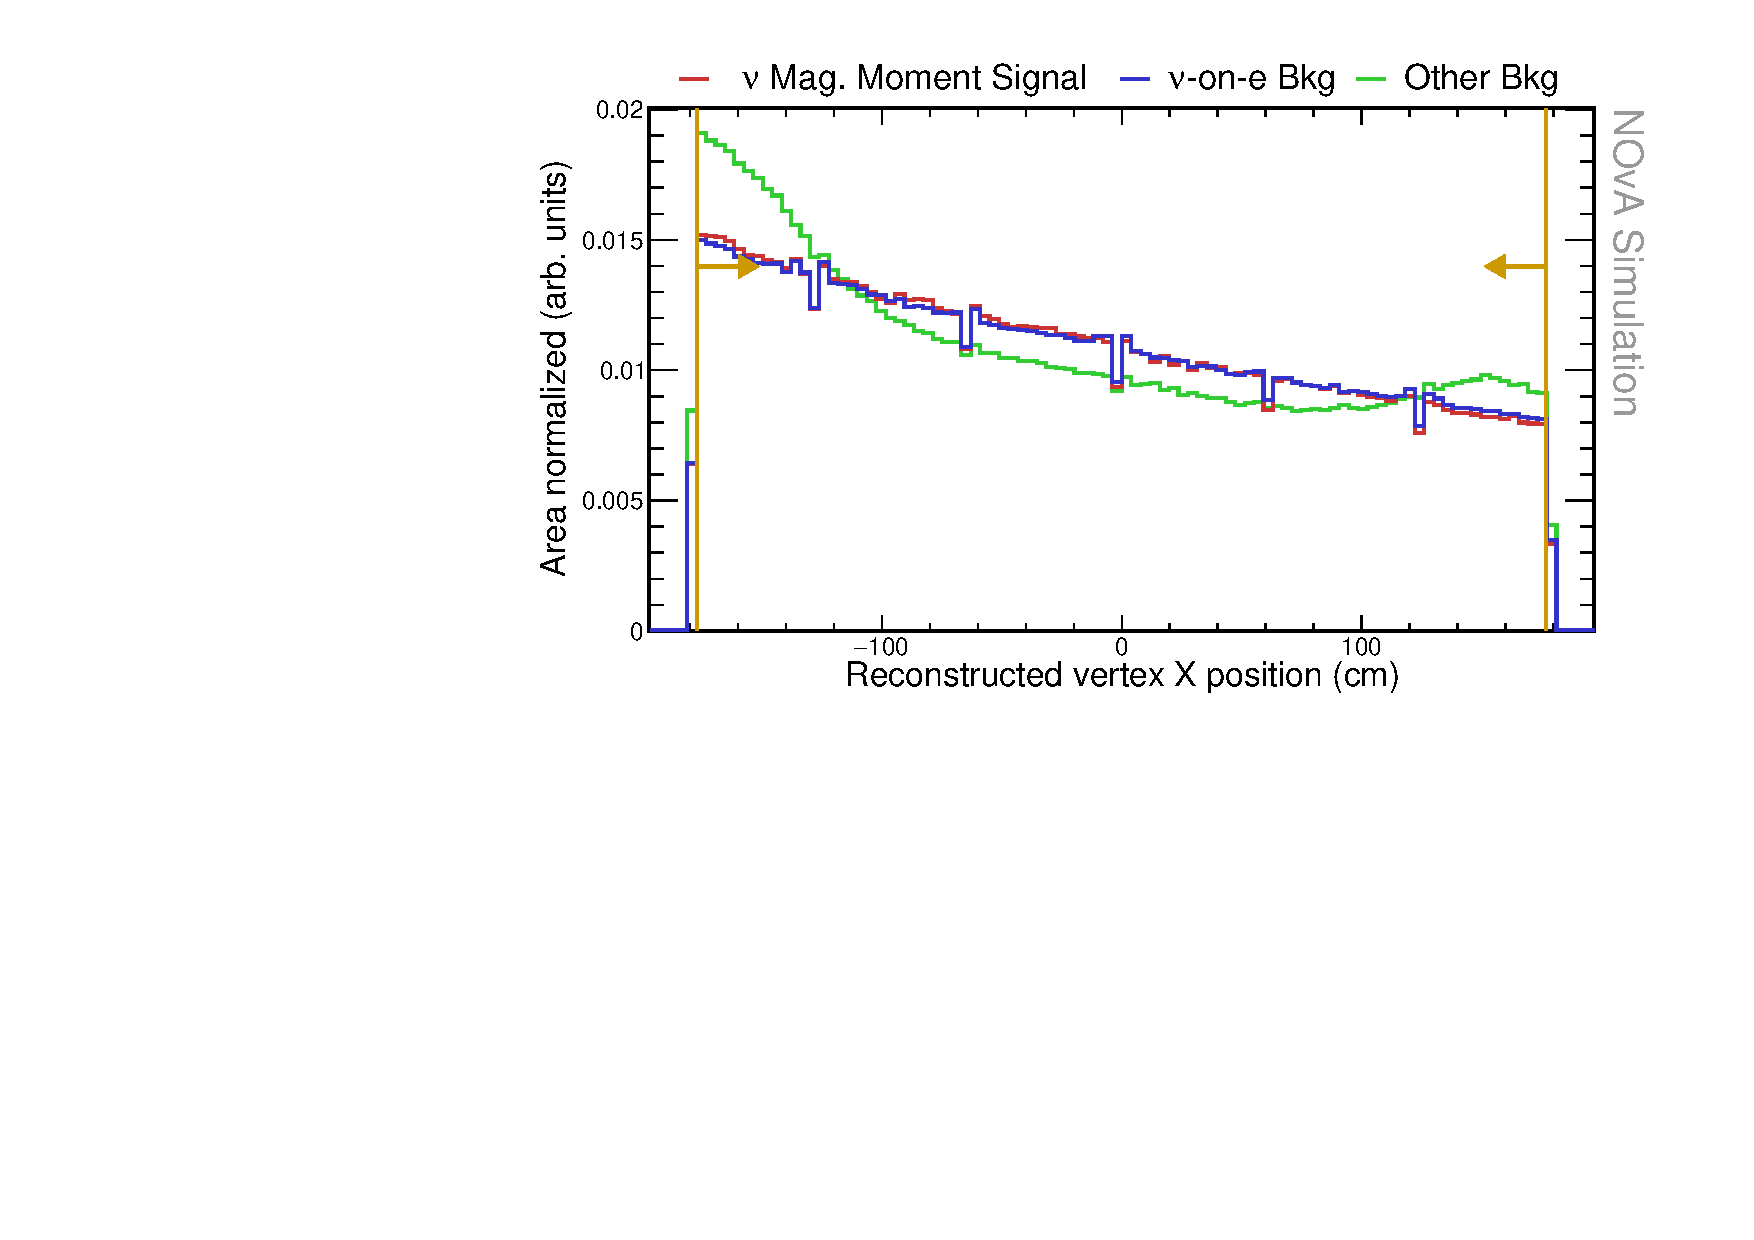
\includegraphics[width=.7\textwidth]{Plots/NuMMEventSelection/N1Cut_vtxXActive.pdf}
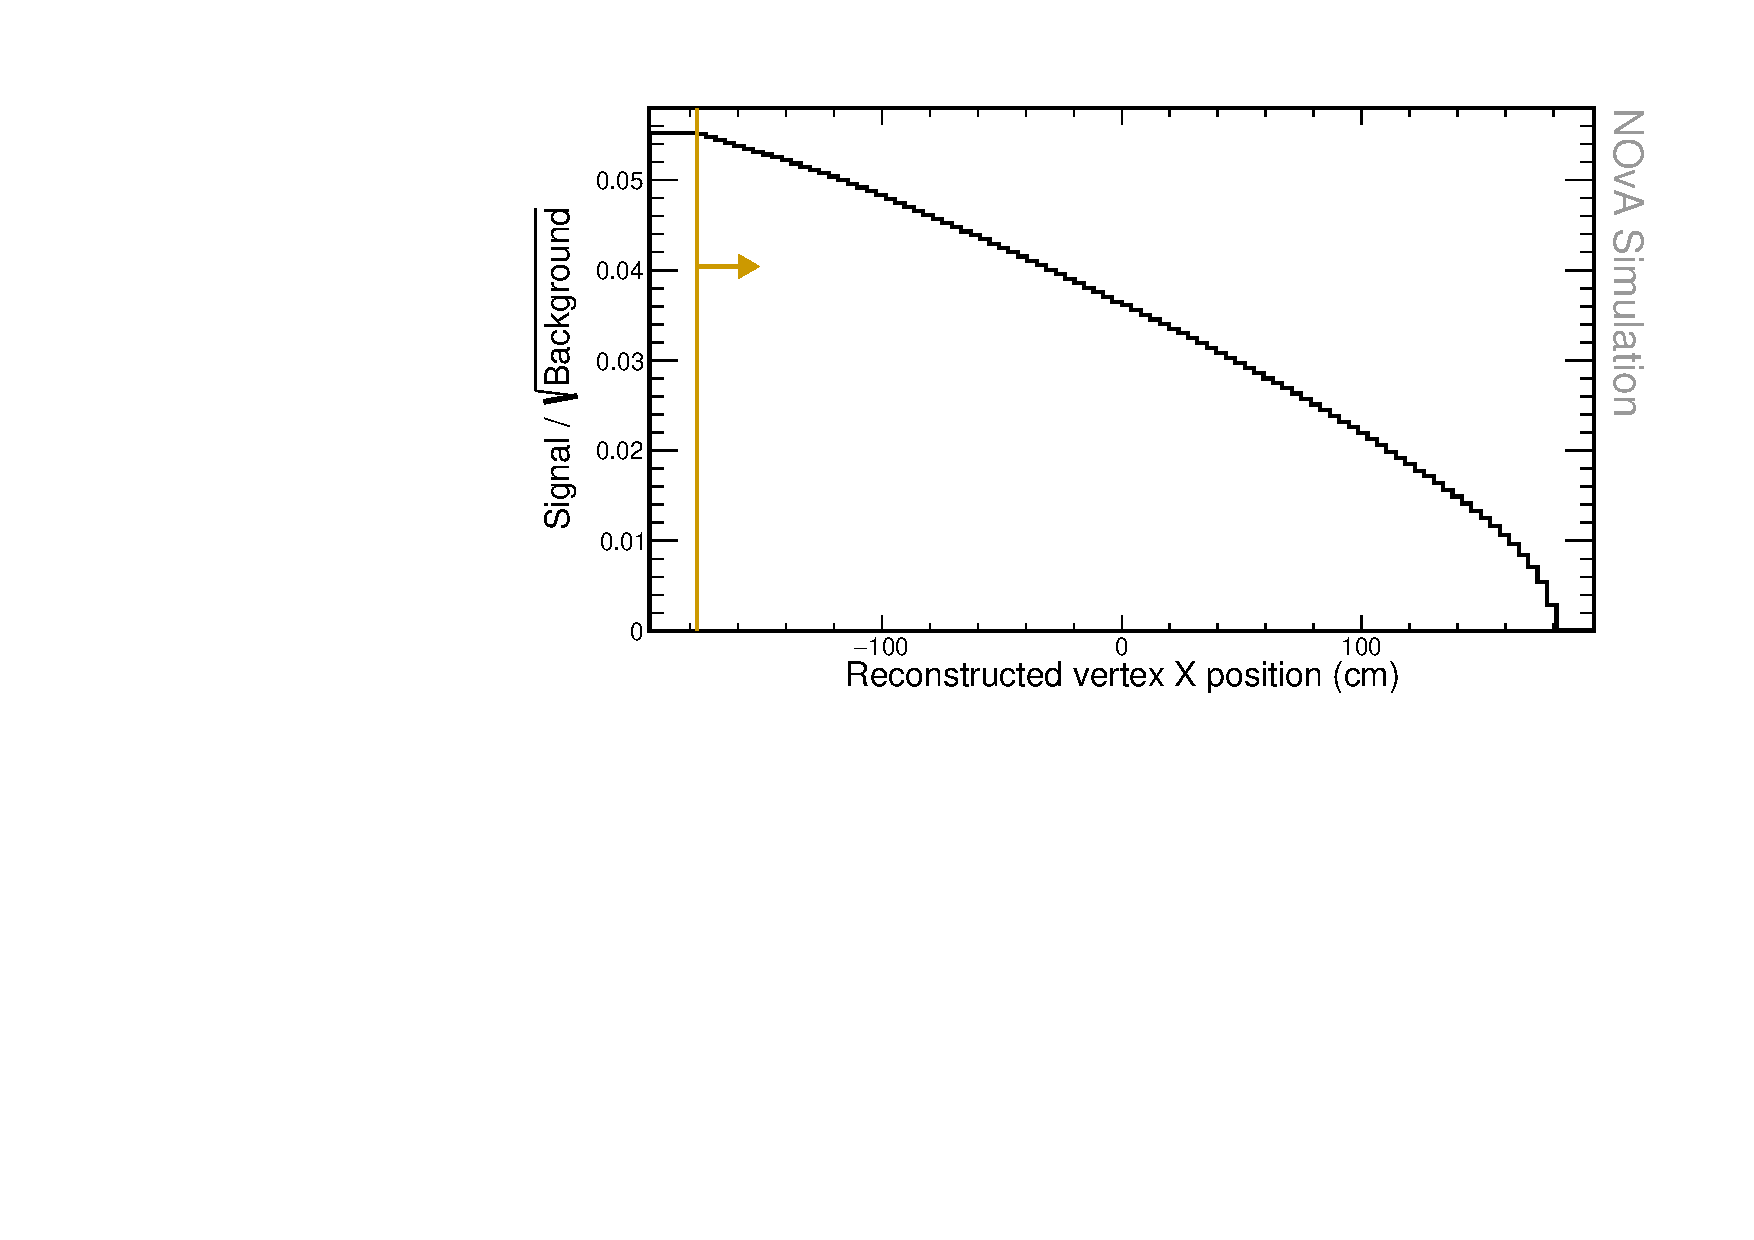
\includegraphics[width=.7\textwidth]{Plots/NuMMEventSelection/NuMM_N1Cut_vtxXActiveright_FOMStats.pdf}
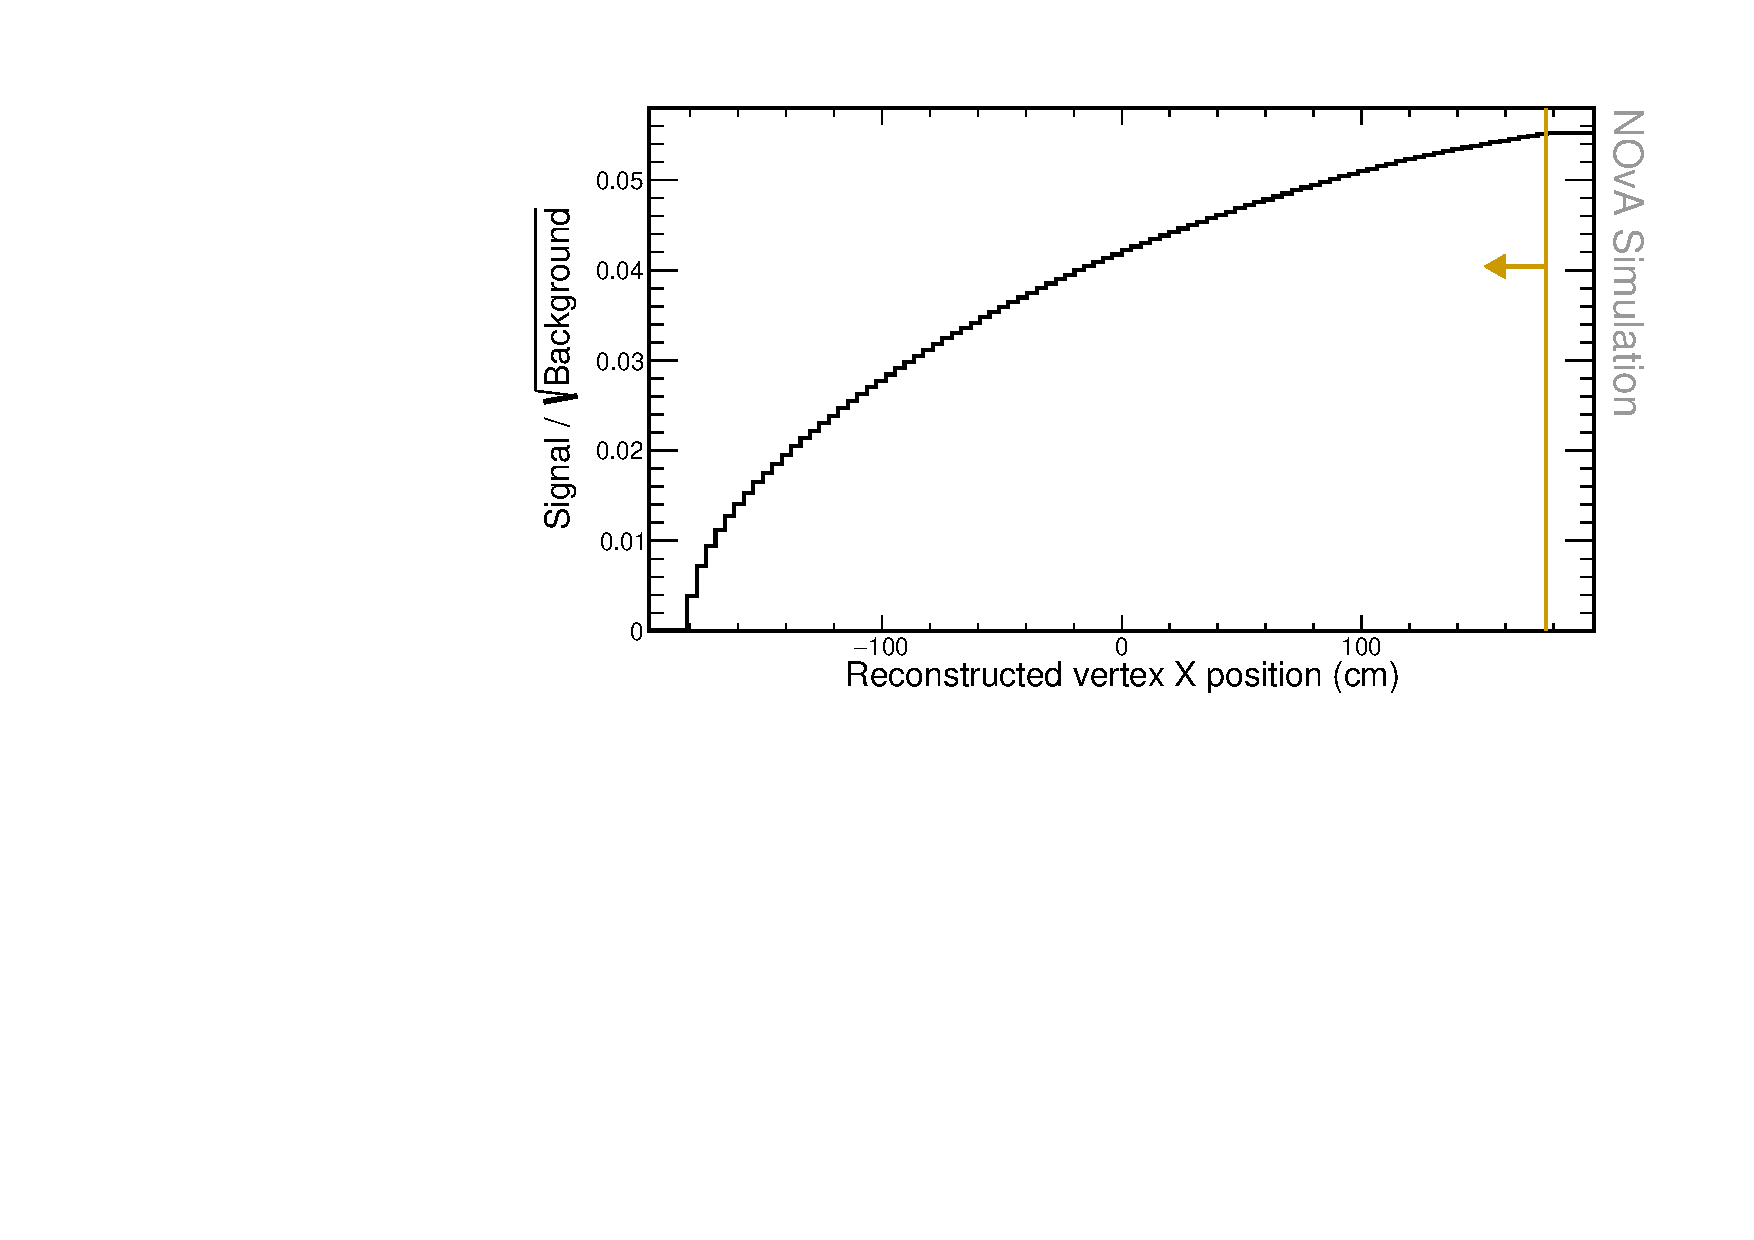
\includegraphics[width=.7\textwidth]{Plots/NuMMEventSelection/NuMM_N1Cut_vtxXActiveleft_FOMStats.pdf}
\caption[Vertex x containment cut]{Top: Relative comparison of signal (red), \acrshort{nuone} background (blue), and other background (green) events in the distribution of the x position of the reconstructed vertex. All histograms are area-normalized. Middle and bottom: Cumulative \acrshort{FOM} calculated as the number of signal events, divided by the number of background events from that bin until the end of the plot to the right (middle) or left (bottom). The reconstruction quality and pre-selection cuts were applied prior to making these plots. Additionally, vertex is required to be within the active region of the detector ($Vtx_Z<\unit[1270]{cm}$). Yellow lines show the cut values that create the fiducial volume, with arrows pointing towards the preserved events.}
\label{fig:NuMMFiducialCutX}
\end{figure}

\begin{figure}[hbtp]
\centering
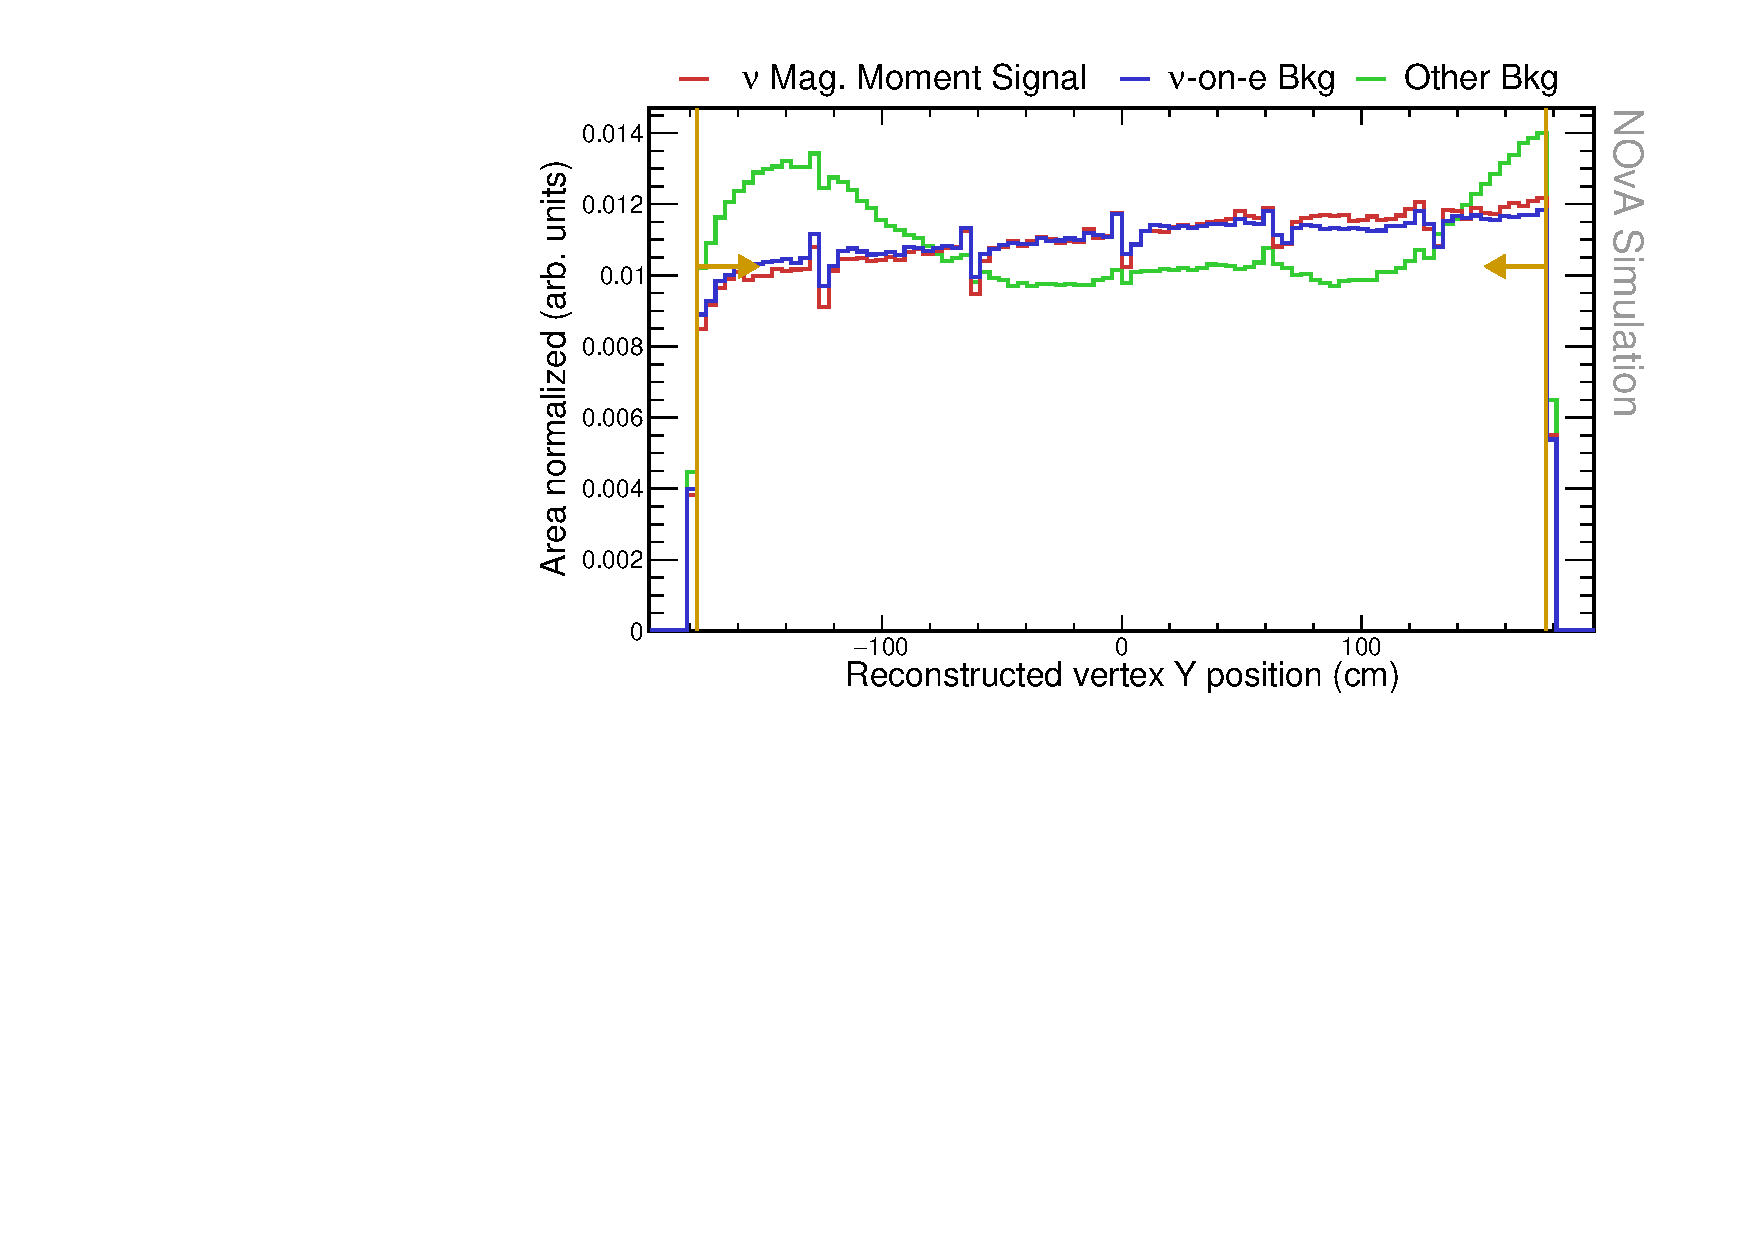
\includegraphics[width=.7\textwidth]{Plots/NuMMEventSelection/N1Cut_vtxYActive.pdf}
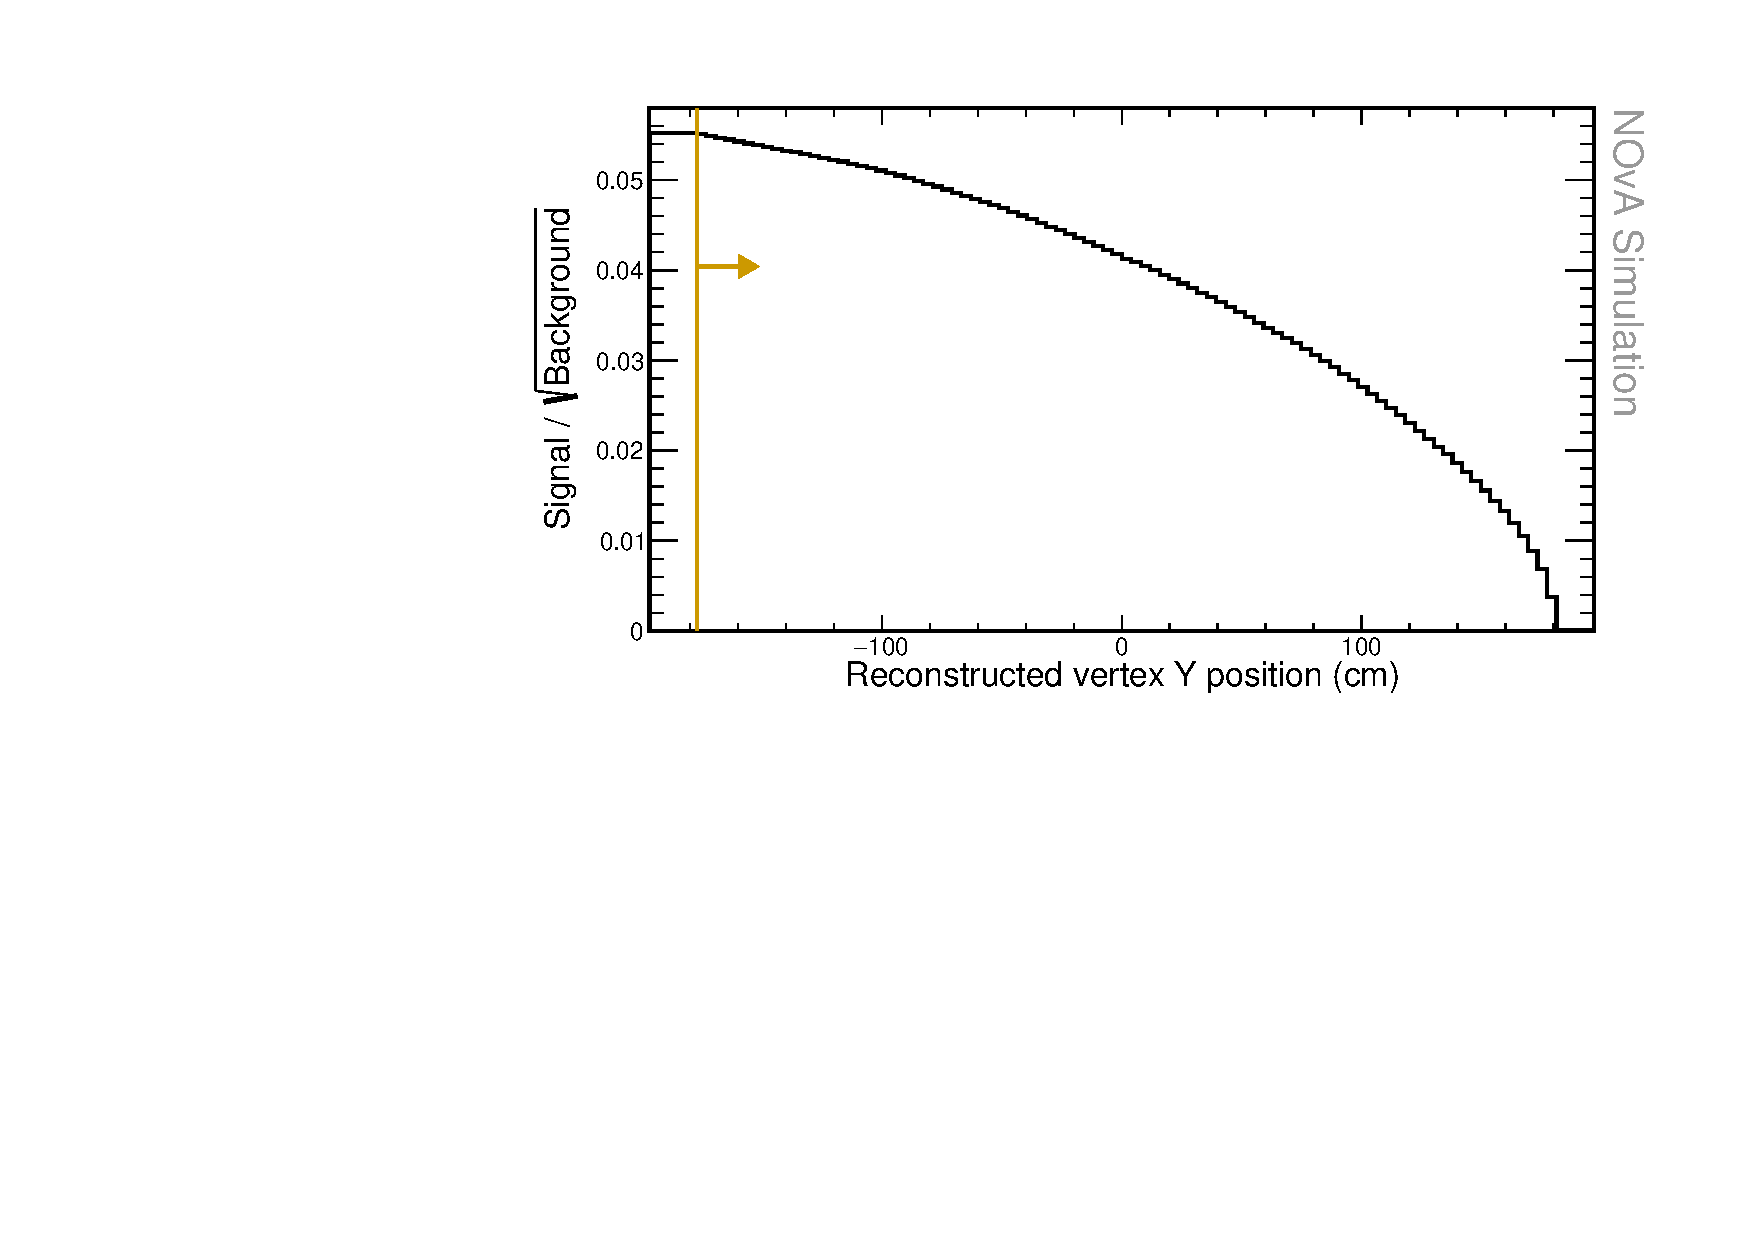
\includegraphics[width=.7\textwidth]{Plots/NuMMEventSelection/NuMM_N1Cut_vtxYActiveright_FOMStats.pdf}
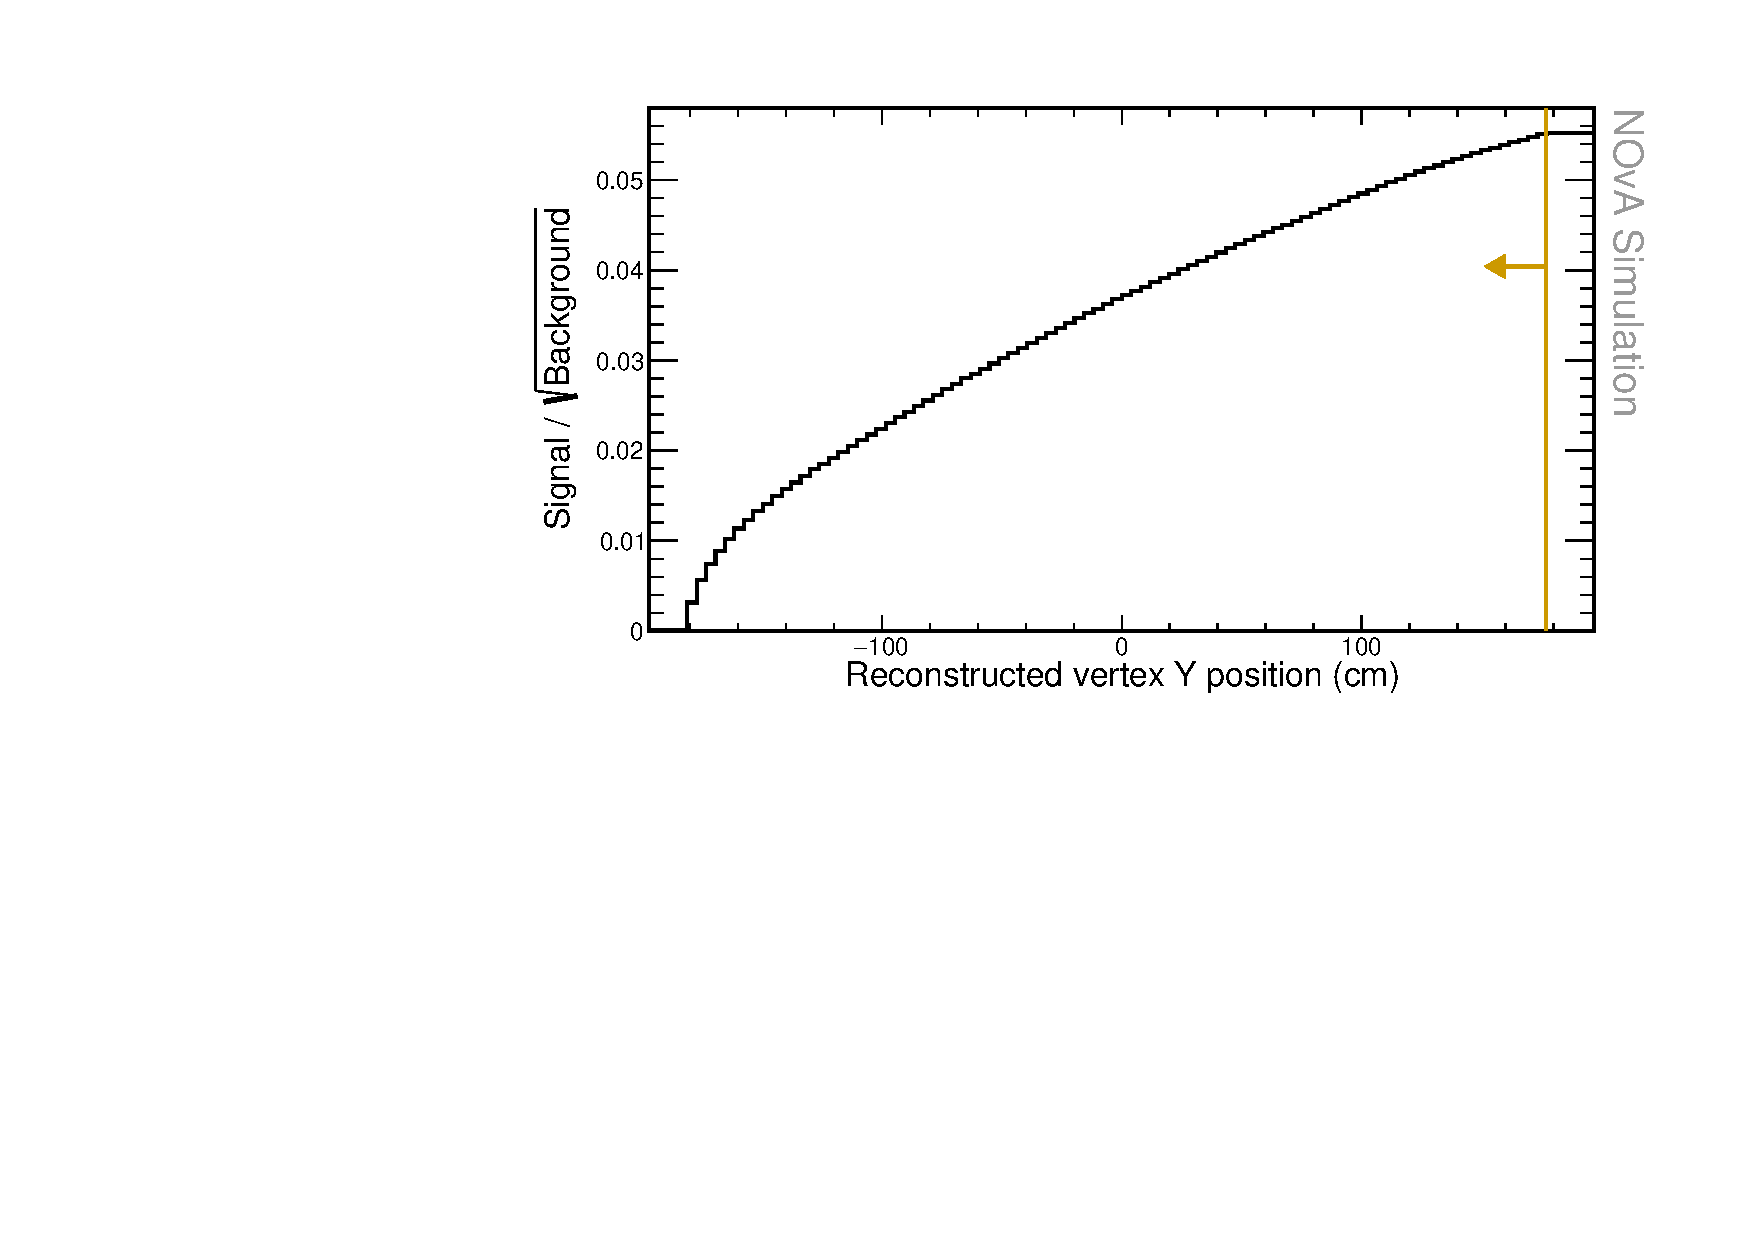
\includegraphics[width=.7\textwidth]{Plots/NuMMEventSelection/NuMM_N1Cut_vtxYActiveleft_FOMStats.pdf}
\caption[Vertex y containment cut]{Top: Relative comparison of signal (red), \acrshort{nuone} background (blue), and other background (green) events in the distribution of the y position of the reconstructed vertex. All histograms are area-normalized. Middle and bottom: Cumulative \acrshort{FOM} calculated as the number of signal events, divided by the number of background events from that bin until the end of the plot to the right (middle) or left (bottom). The reconstruction quality and pre-selection cuts were applied prior to making these plots. Additionally, vertex is required to be within the active region of the detector ($Vtx_Z<\unit[1270]{cm}$). Yellow lines show the cut values that create the fiducial volume, with arrows pointing towards the preserved events.}
\label{fig:NuMMFiducialCutY}
\end{figure}

\begin{figure}[hbtp]
\centering
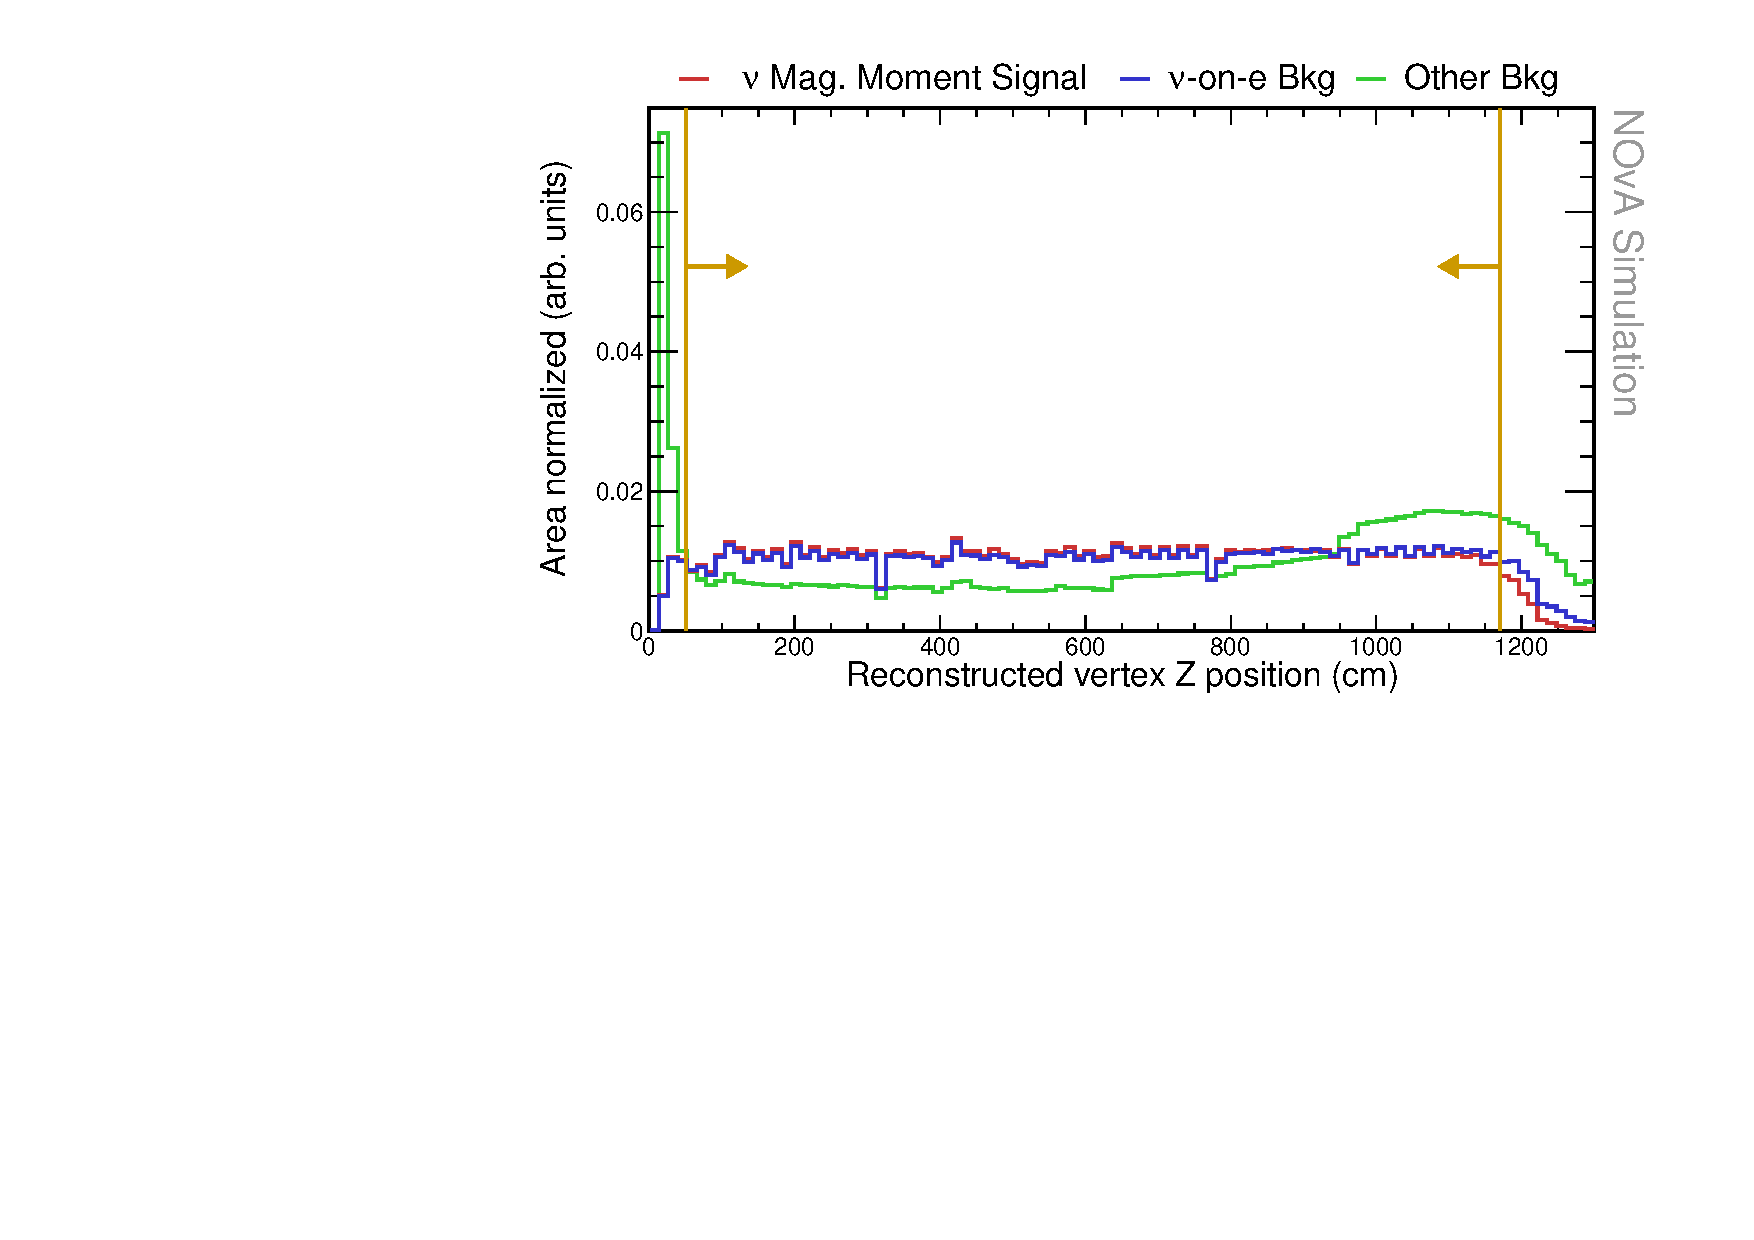
\includegraphics[width=.7\textwidth]{Plots/NuMMEventSelection/N1Cut_vtxZ.pdf}
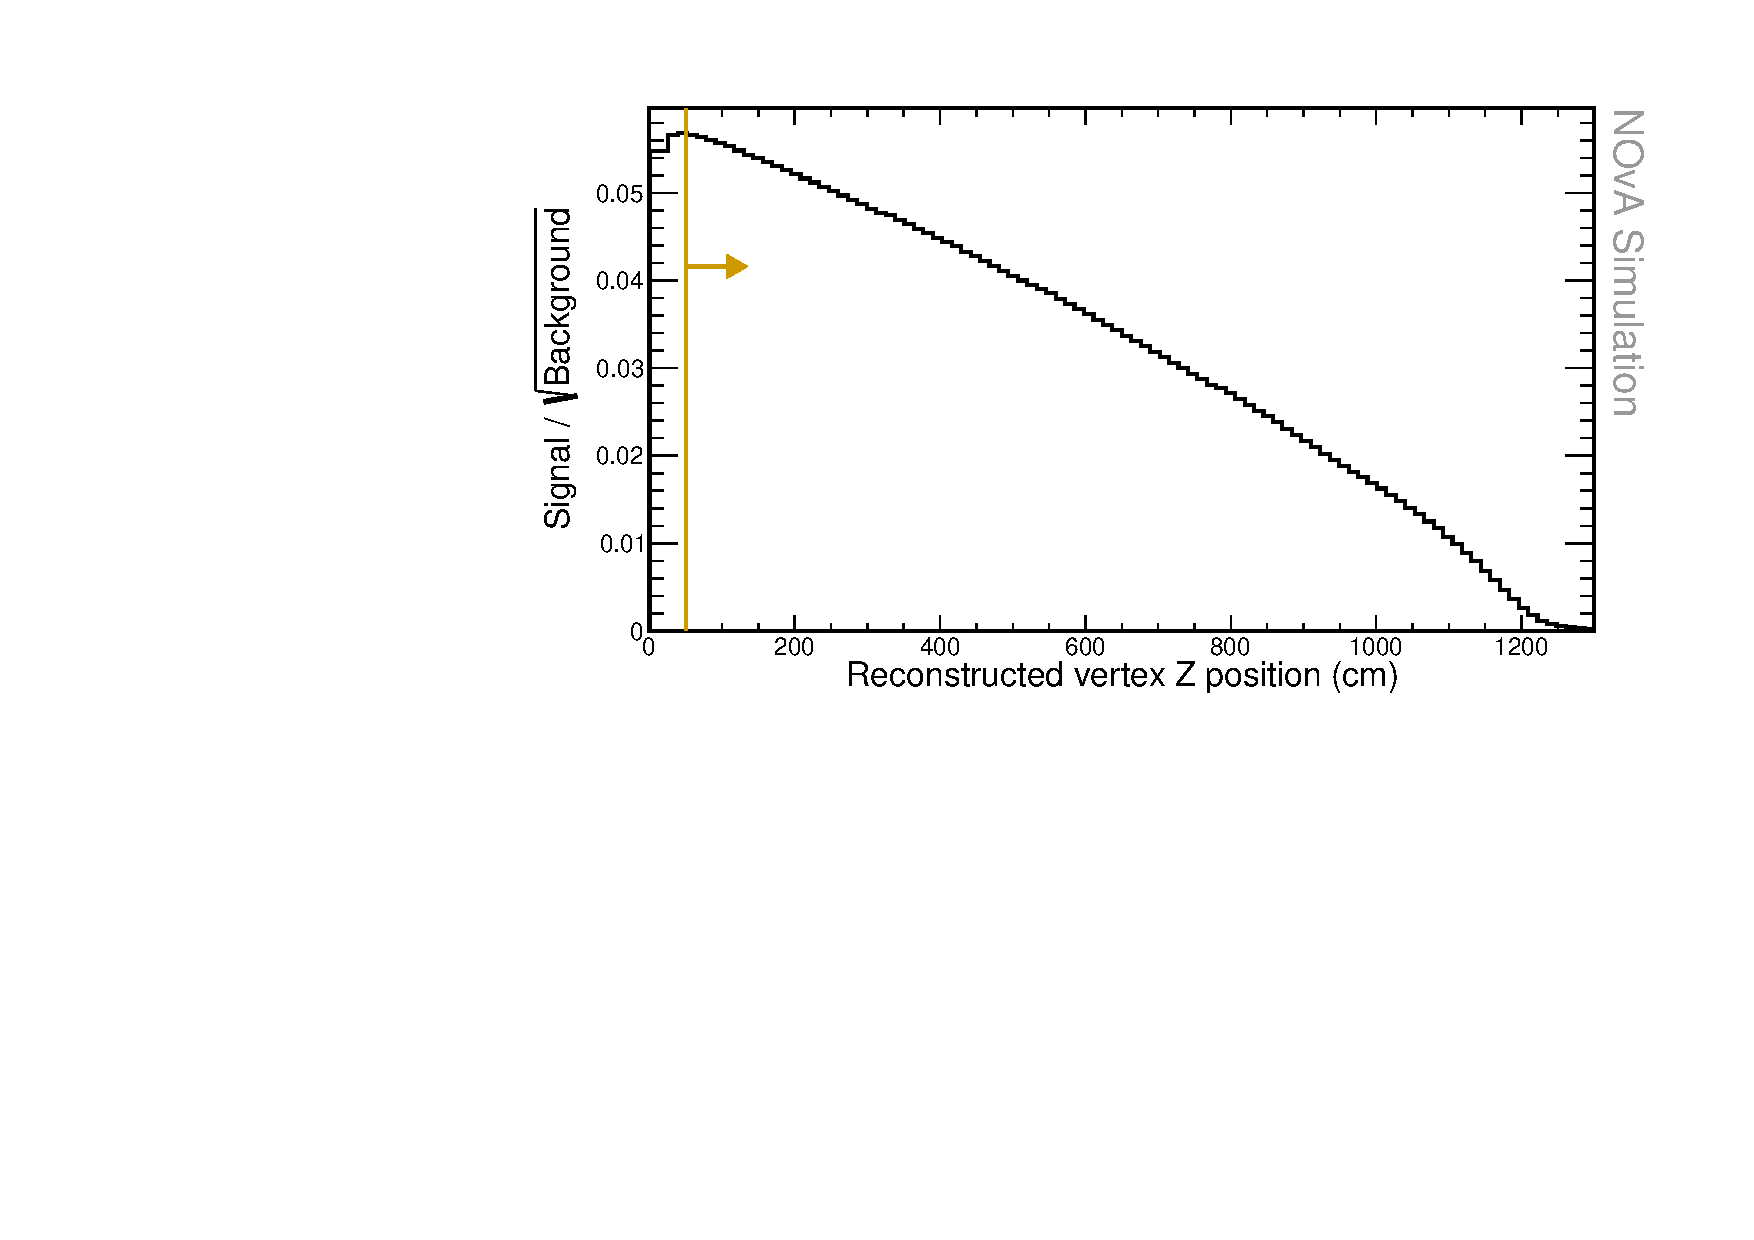
\includegraphics[width=.7\textwidth]{Plots/NuMMEventSelection/NuMM_N1Cut_vtxZright_FOMStats.pdf}
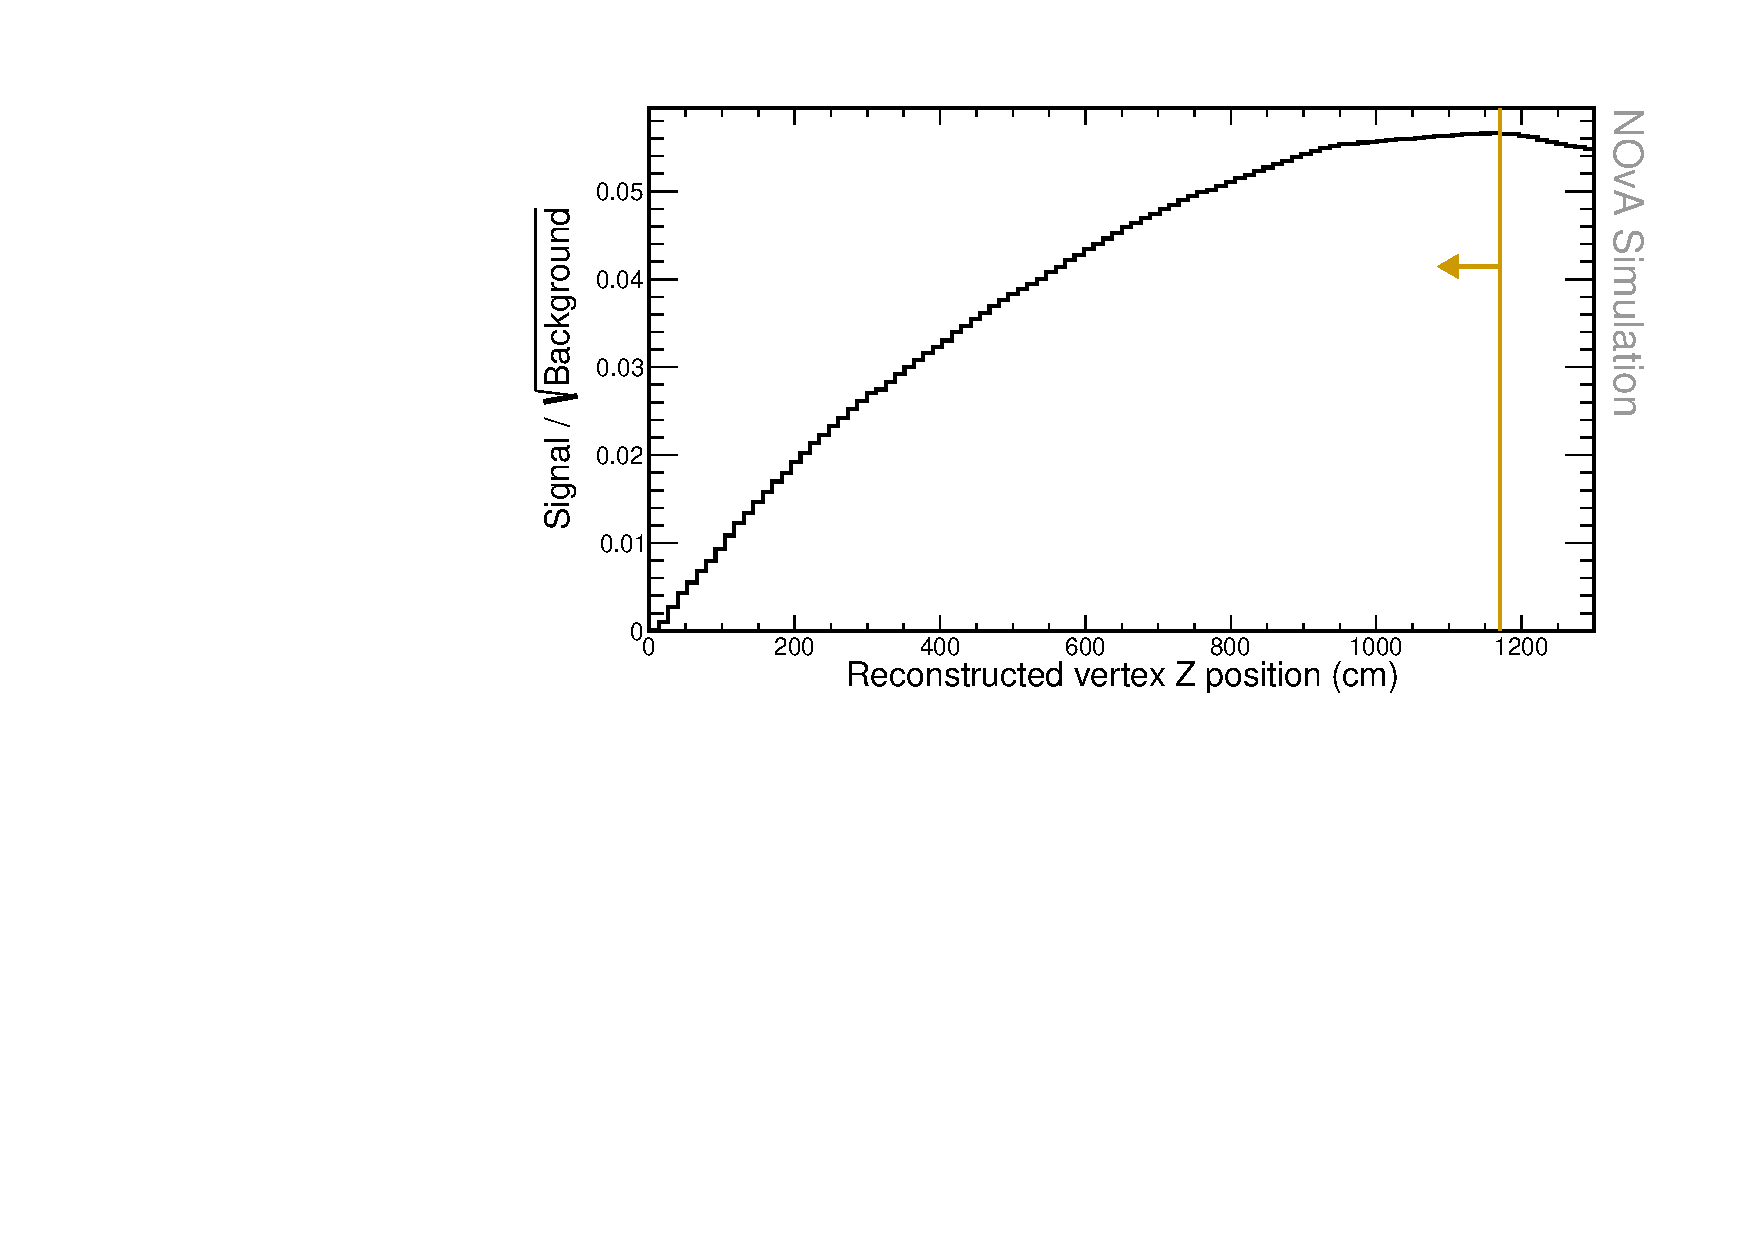
\includegraphics[width=.7\textwidth]{Plots/NuMMEventSelection/NuMM_N1Cut_vtxZleft_FOMStats.pdf}
\caption[Vertex z containment cut]{Top: Relative comparison of signal (red), \acrshort{nuone} background (blue), and other background (green) events in the distribution of the z position of the reconstructed vertex. All histograms are area-normalized. Middle and bottom: Cumulative \acrshort{FOM} calculated as the number of signal events, divided by the number of background events from that bin until the end of the plot to the right (middle) or left (bottom). The reconstruction quality and pre-selection cuts were applied prior to making these plots. Yellow lines show the cut values that create the fiducial volume, with arrows pointing towards the preserved events.}
\label{fig:NuMMFiducialCutZ}
\end{figure}

Furthermore, we constrain the extreme positions (minimum and maximum) of all the hits within the most energetic prong, which is assumed to represent the electron shower for the signal events. We apply the reconstruction quality, pre-selection and fiducial (vertex position) cuts to their distributions, shown in Fig.~\ref{fig:NuMMContainmentCutMinX}-\ref{fig:NuMMContainmentCutMaxZ}. The extreme hit positions are required to be within the following volume: 
\begin{align}
\unit[-175]{cm}<\textsf{min}_X,& \textsf{max}_X<\unit[175]{cm},\\
\unit[-175]{cm}<\textsf{min}_Y,& \textsf{max}_Y<\unit[175]{cm},\\
\unit[105]{cm}<\textsf{min}_Z,& \textsf{max}_Z<\unit[1270]{cm}.
\end{align}

\begin{figure}[hbtp]
\centering
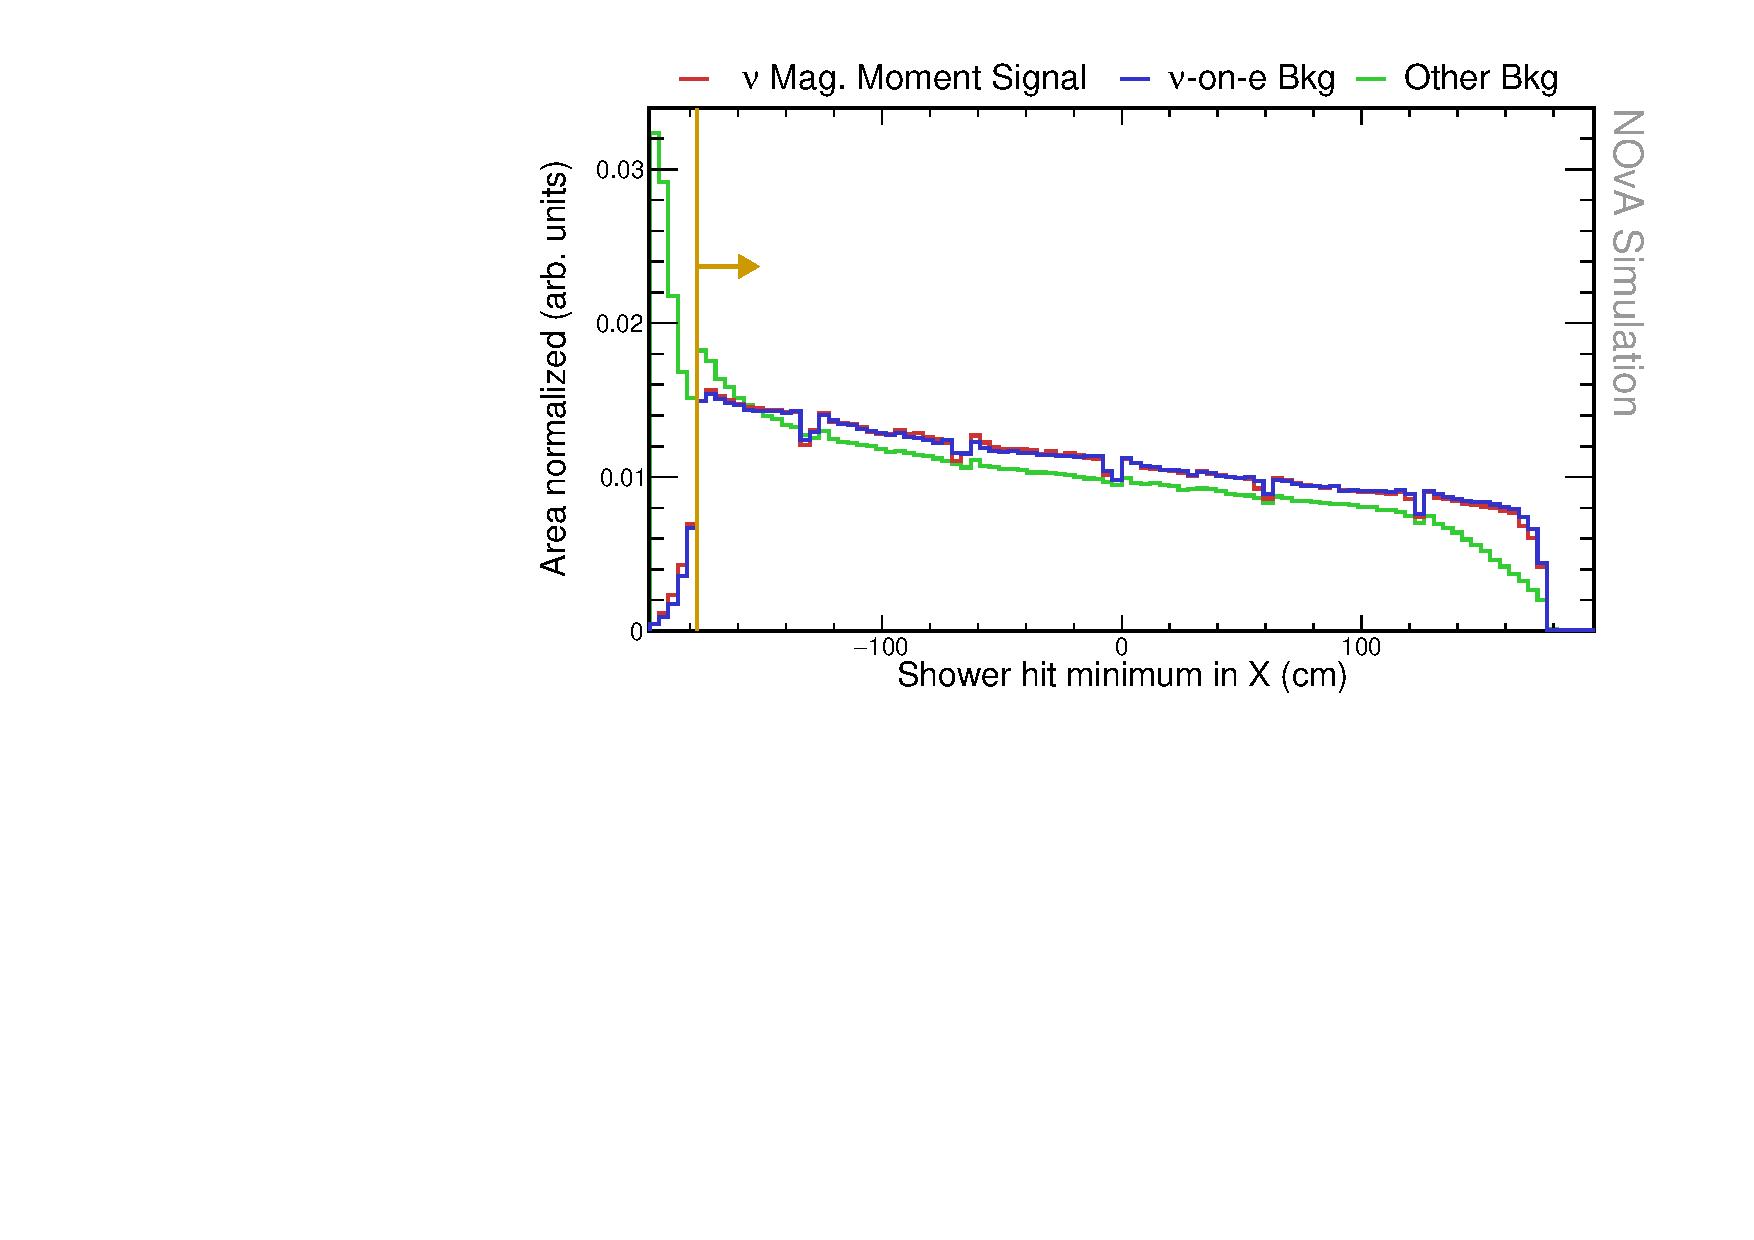
\includegraphics[width=.7\textwidth]{Plots/NuMMEventSelection/N1Cut_minX.pdf}
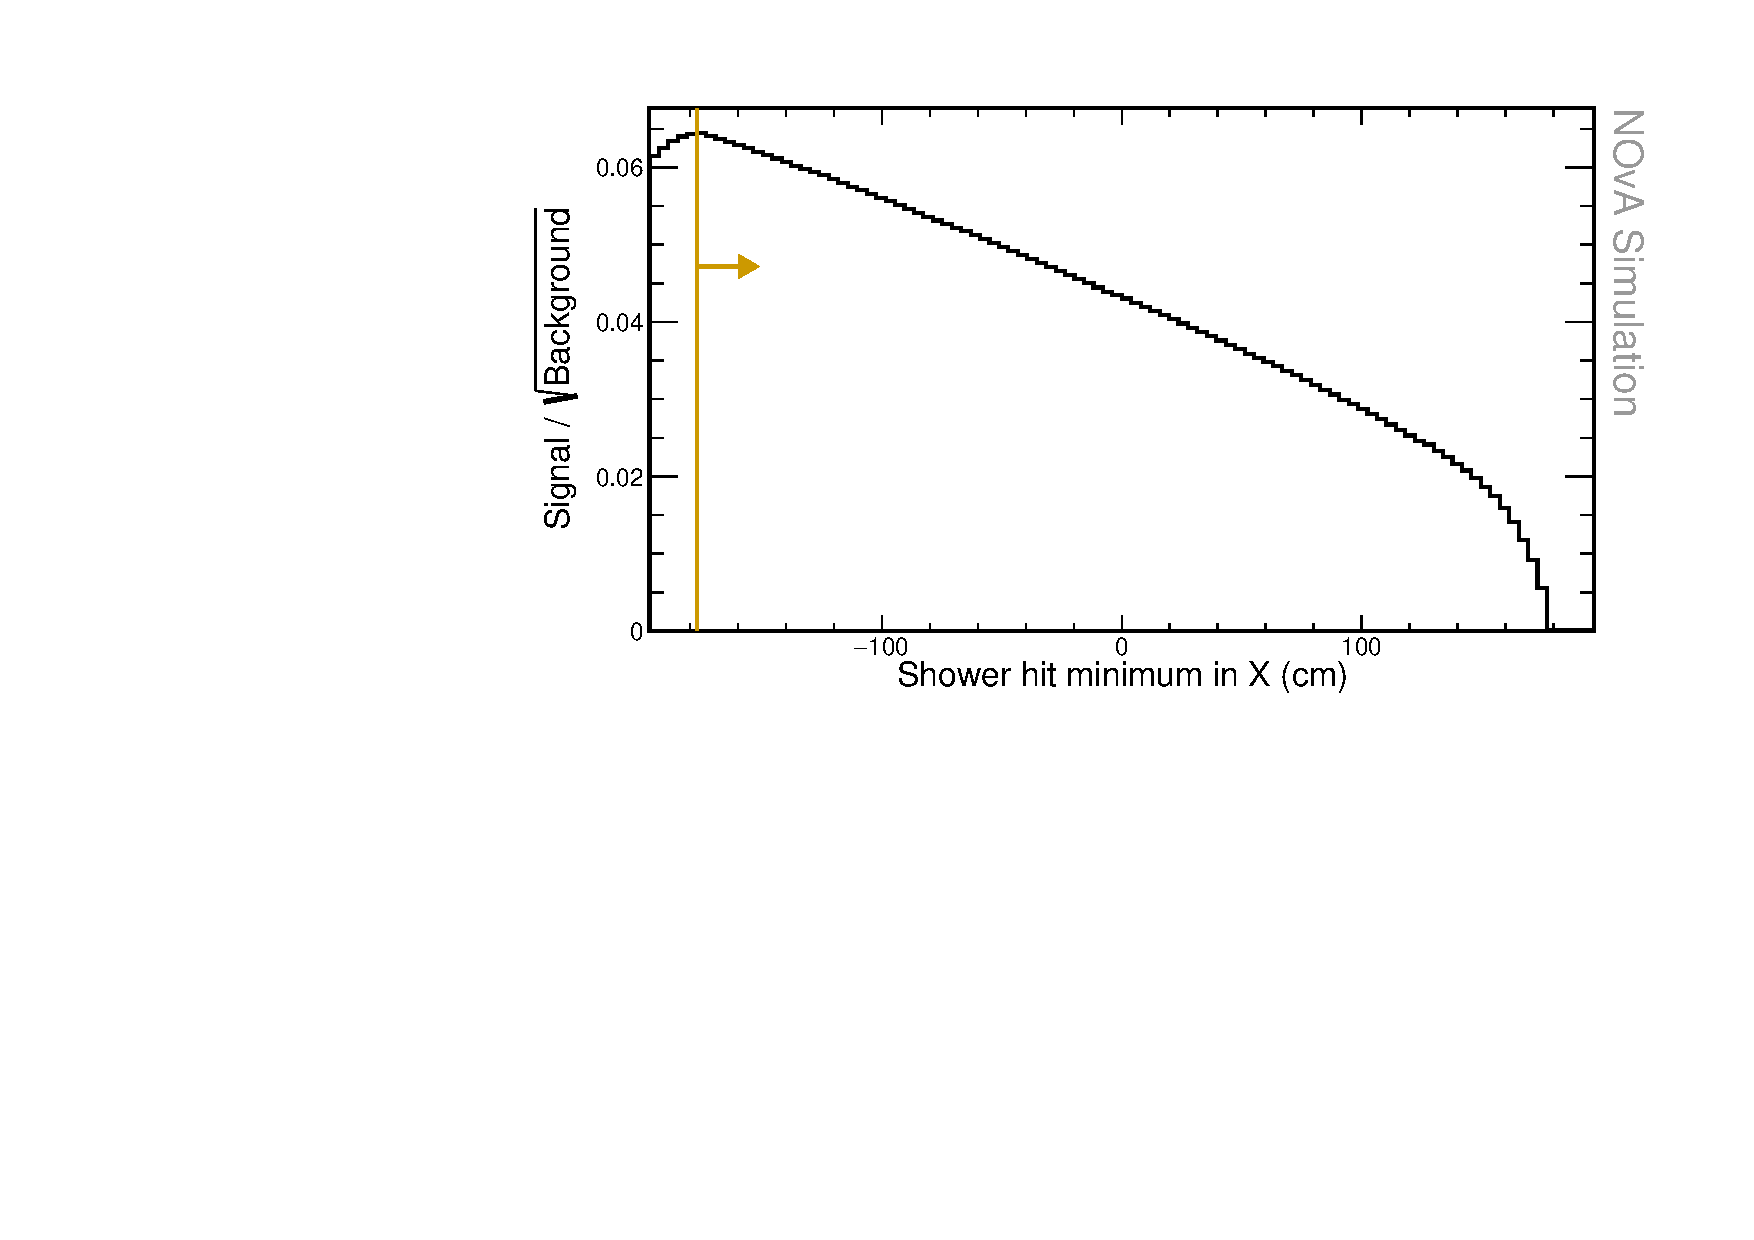
\includegraphics[width=.7\textwidth]{Plots/NuMMEventSelection/NuMM_N1Cut_minXright_FOMStats.pdf}
\caption[Hit minimum x containment cut]{Top: Relative comparison of signal (red), \acrshort{nuone} background (blue), and other background (green) events in the distribution of the minimum hit position of the most energetic prong along the x axis. All histograms are area-normalized. Bottom: Cumulative \acrshort{FOM} calculated as the number of signal events, divided by the number of background events from that bin until the end of the plot in the direction of the yellow arrow. The reconstruction quality, pre-selection and fiducial cuts were applied prior to making these plots. Yellow lines show the cut values that create the containment volume, with arrows pointing towards the preserved events.}
\label{fig:NuMMContainmentCutMinX}
\end{figure}

\begin{figure}[hbtp]
\centering
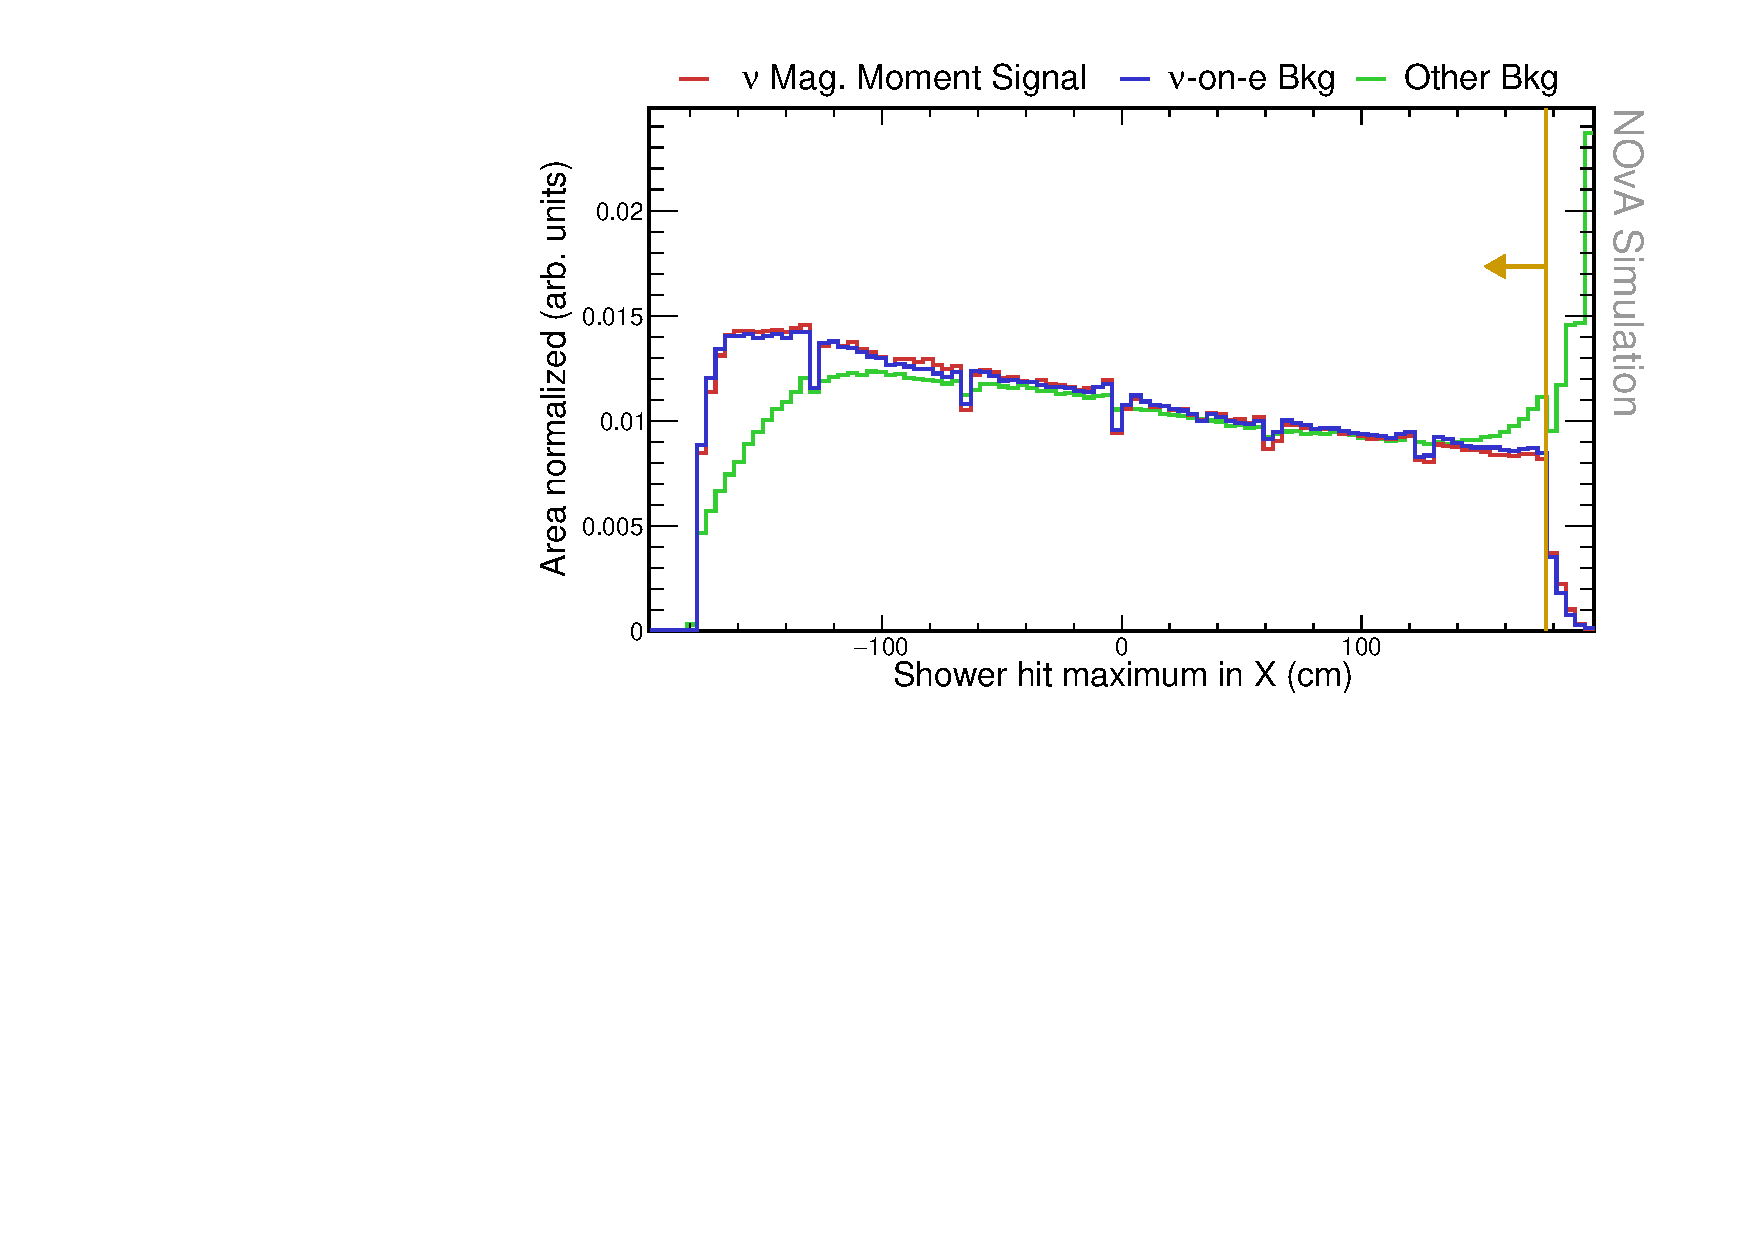
\includegraphics[width=.7\textwidth]{Plots/NuMMEventSelection/N1Cut_maxX.pdf}
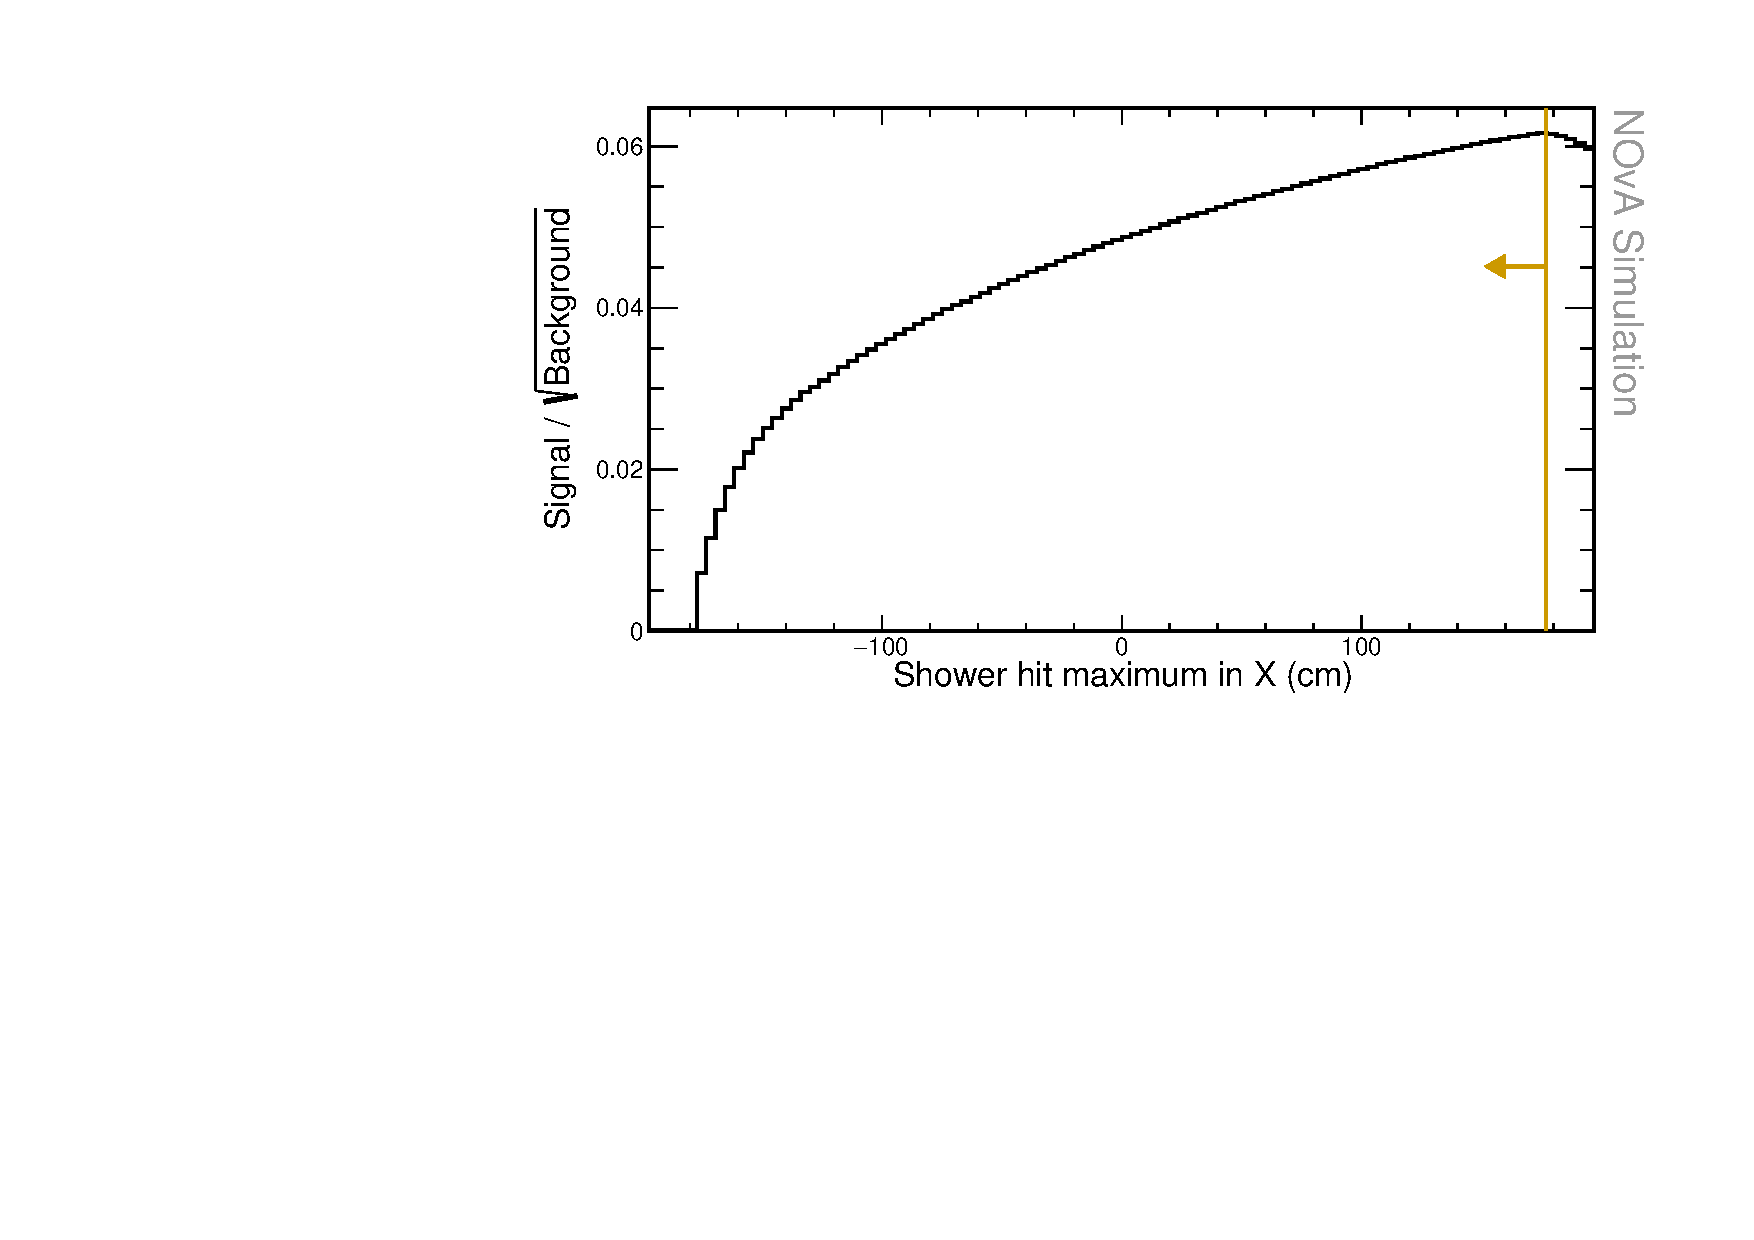
\includegraphics[width=.7\textwidth]{Plots/NuMMEventSelection/NuMM_N1Cut_maxXleft_FOMStats}
\caption[Hit maximum x containment cut]{Top: Relative comparison of signal (red), \acrshort{nuone} background (blue), and other background (green) events in the distribution of the maximum hit position of the most energetic prong along the x axis. All histograms are area-normalized. Bottom: Cumulative \acrshort{FOM} calculated as the number of signal events, divided by the number of background events from that bin until the end of the plot in the direction of the yellow arrow. The reconstruction quality, pre-selection and fiducial cuts were applied prior to making these plots. Yellow lines show the cut values that create the containment volume, with arrows pointing towards the preserved events.}
\label{fig:NuMMContainmentCutMaxX}
\end{figure}

\begin{figure}[hbtp]
\centering
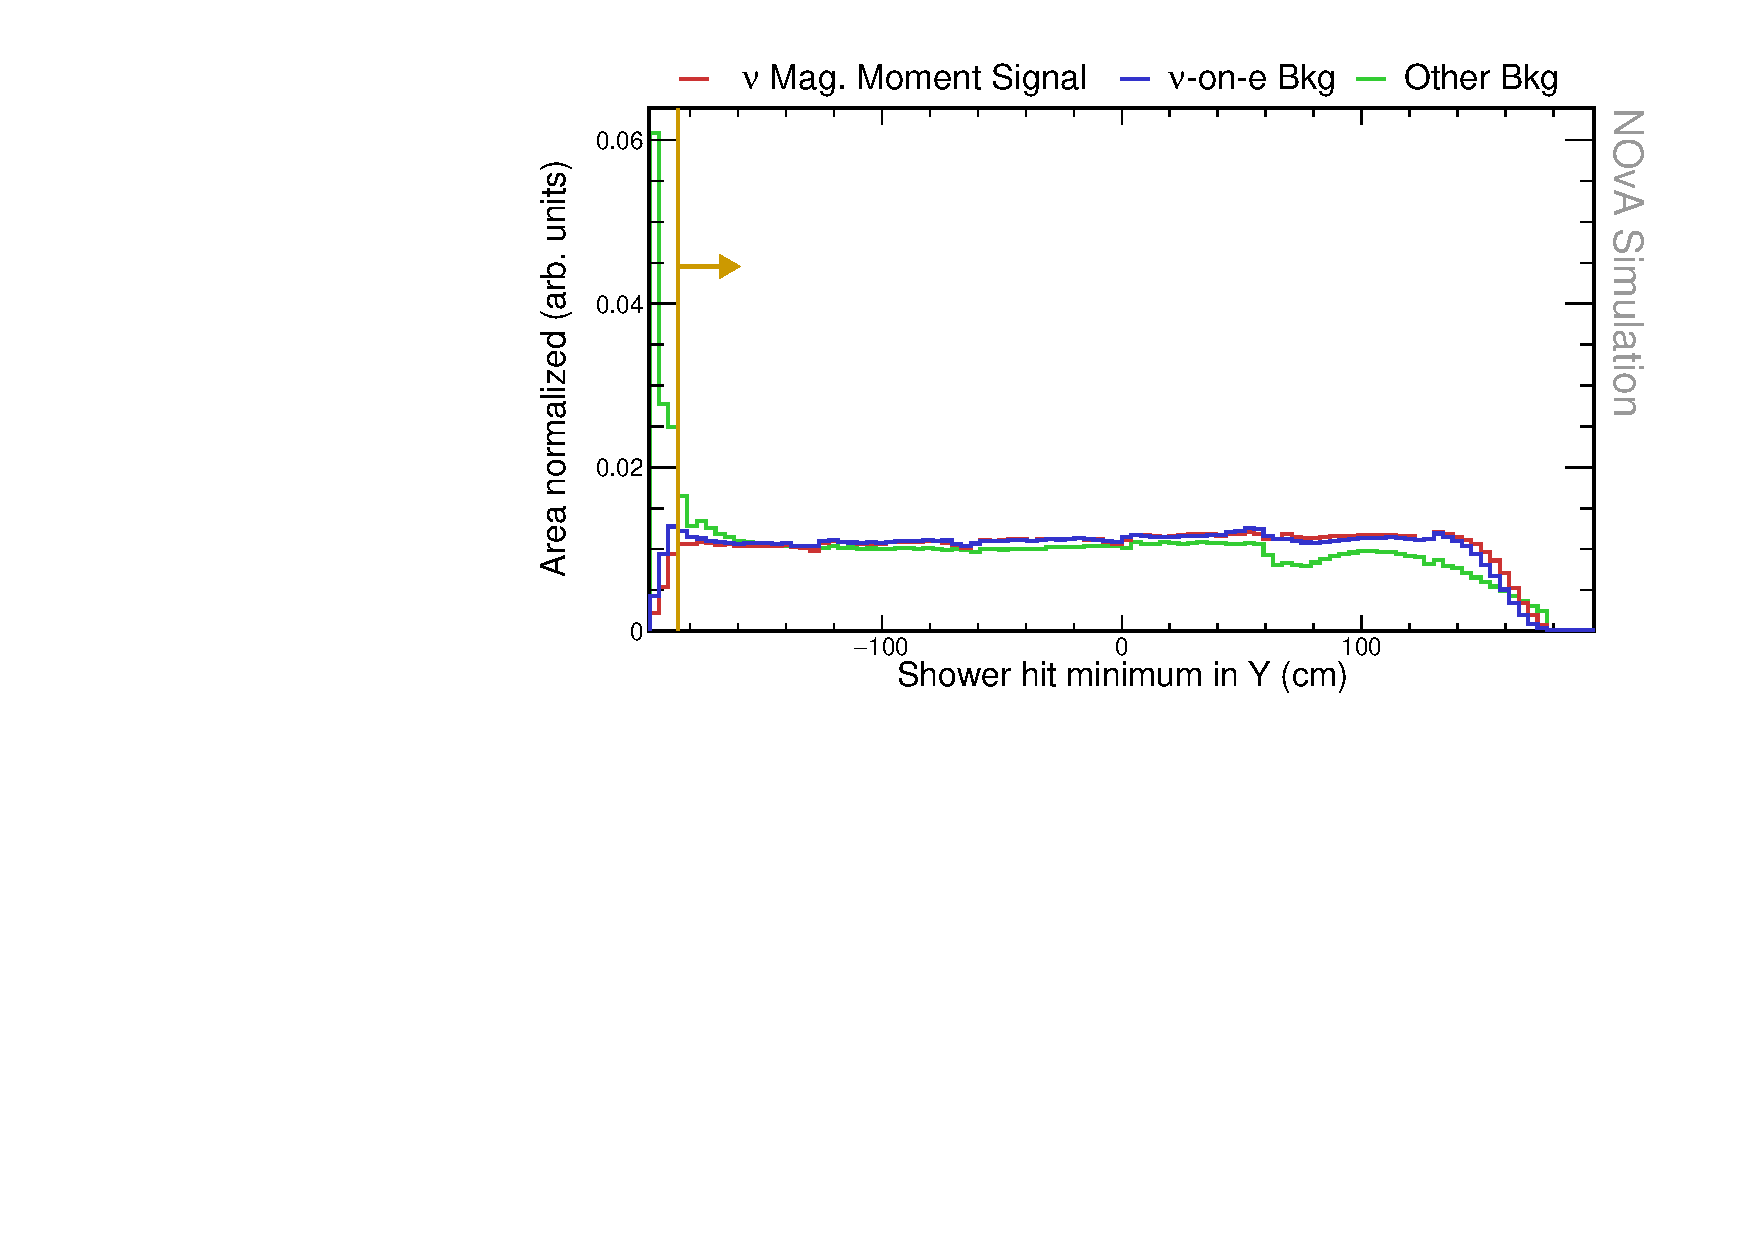
\includegraphics[width=.7\textwidth]{Plots/NuMMEventSelection/N1Cut_minY.pdf}
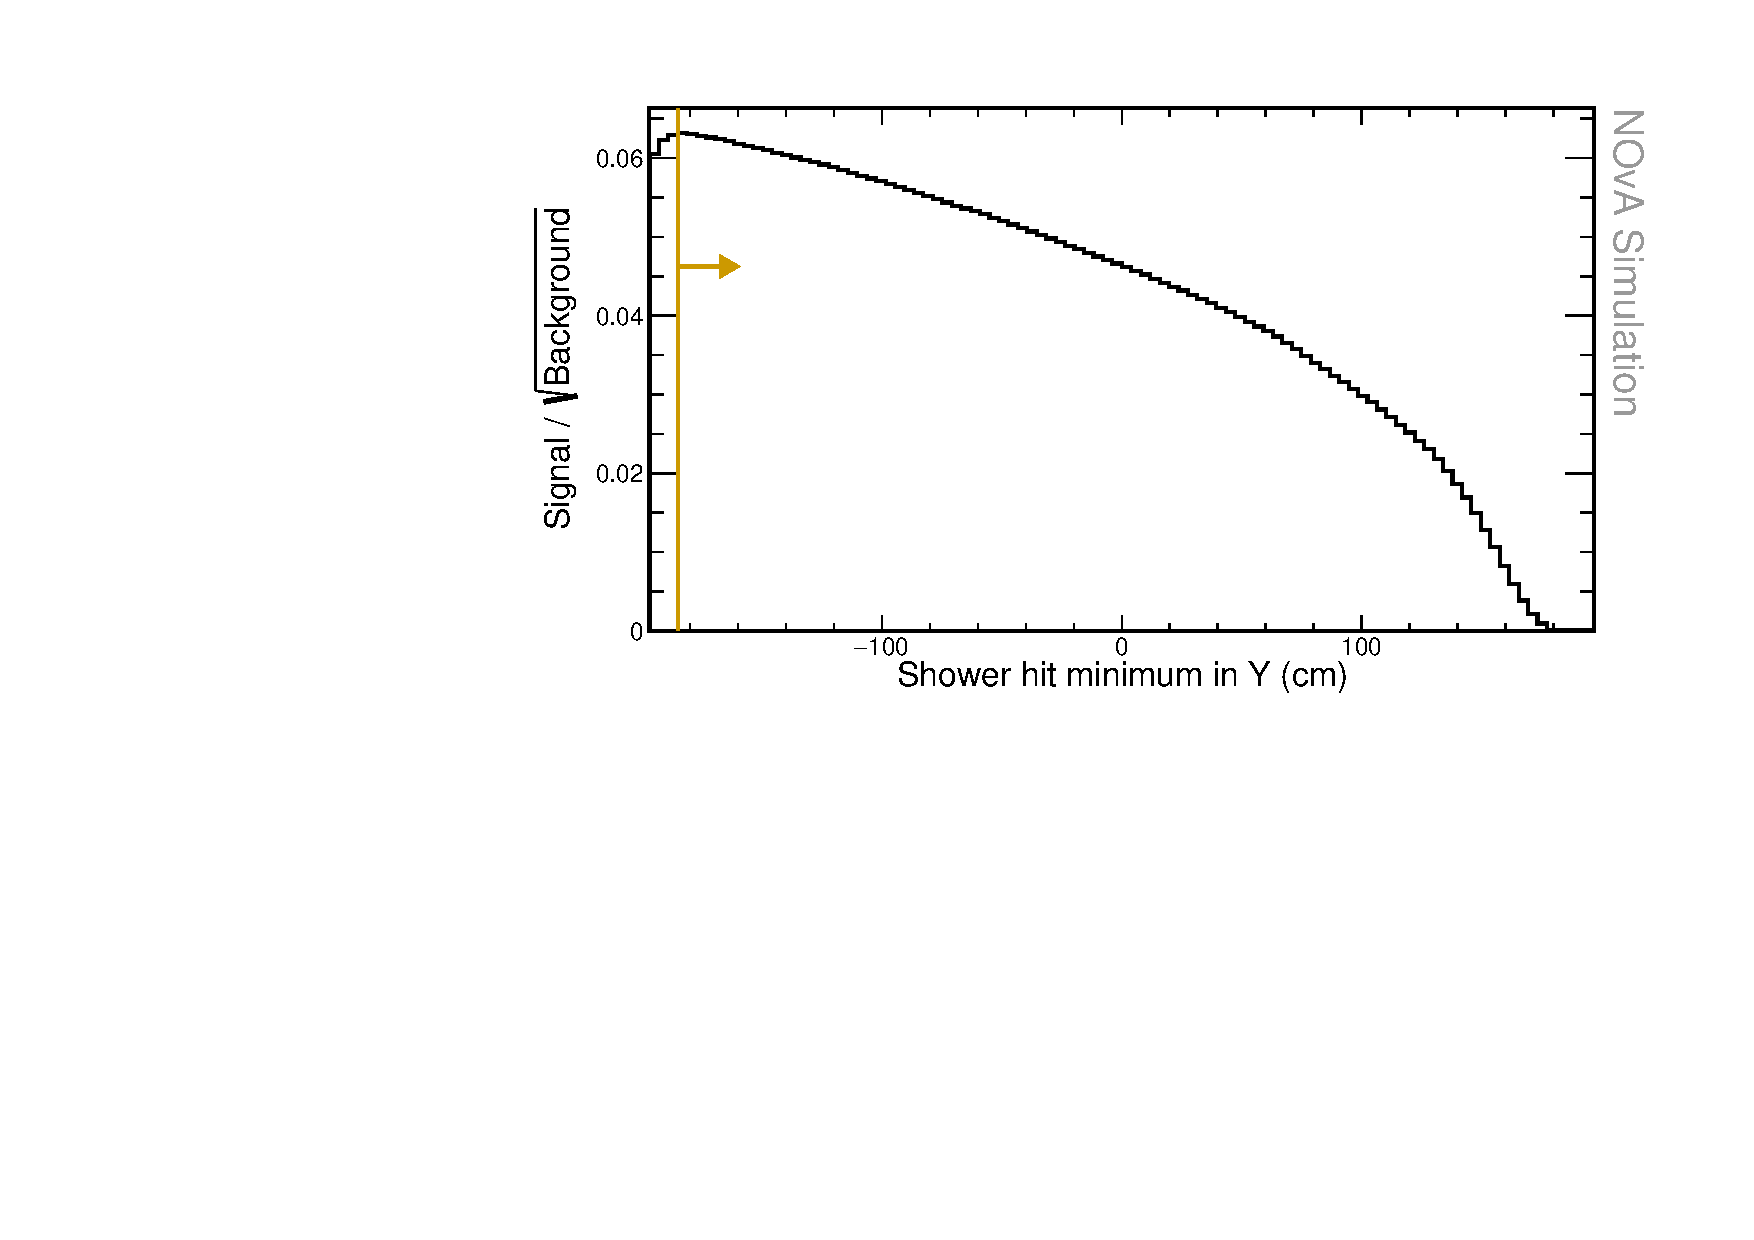
\includegraphics[width=.7\textwidth]{Plots/NuMMEventSelection/NuMM_N1Cut_minYright_FOMStats.pdf}
\caption[Hit minimum y containment cut]{Top: Relative comparison of signal (red), \acrshort{nuone} background (blue), and other background (green) events in the distribution of the minimum hit position of the most energetic prong along the y axis. All histograms are area-normalized. Bottom: Cumulative \acrshort{FOM} calculated as the number of signal events, divided by the number of background events from that bin until the end of the plot in the direction of the yellow arrow. The reconstruction quality, pre-selection and fiducial cuts were applied prior to making these plots. Yellow lines show the cut values that create the containment volume, with arrows pointing towards the preserved events.}
\label{fig:NuMMContainmentCutMinY}
\end{figure}

\begin{figure}[hbtp]
\centering
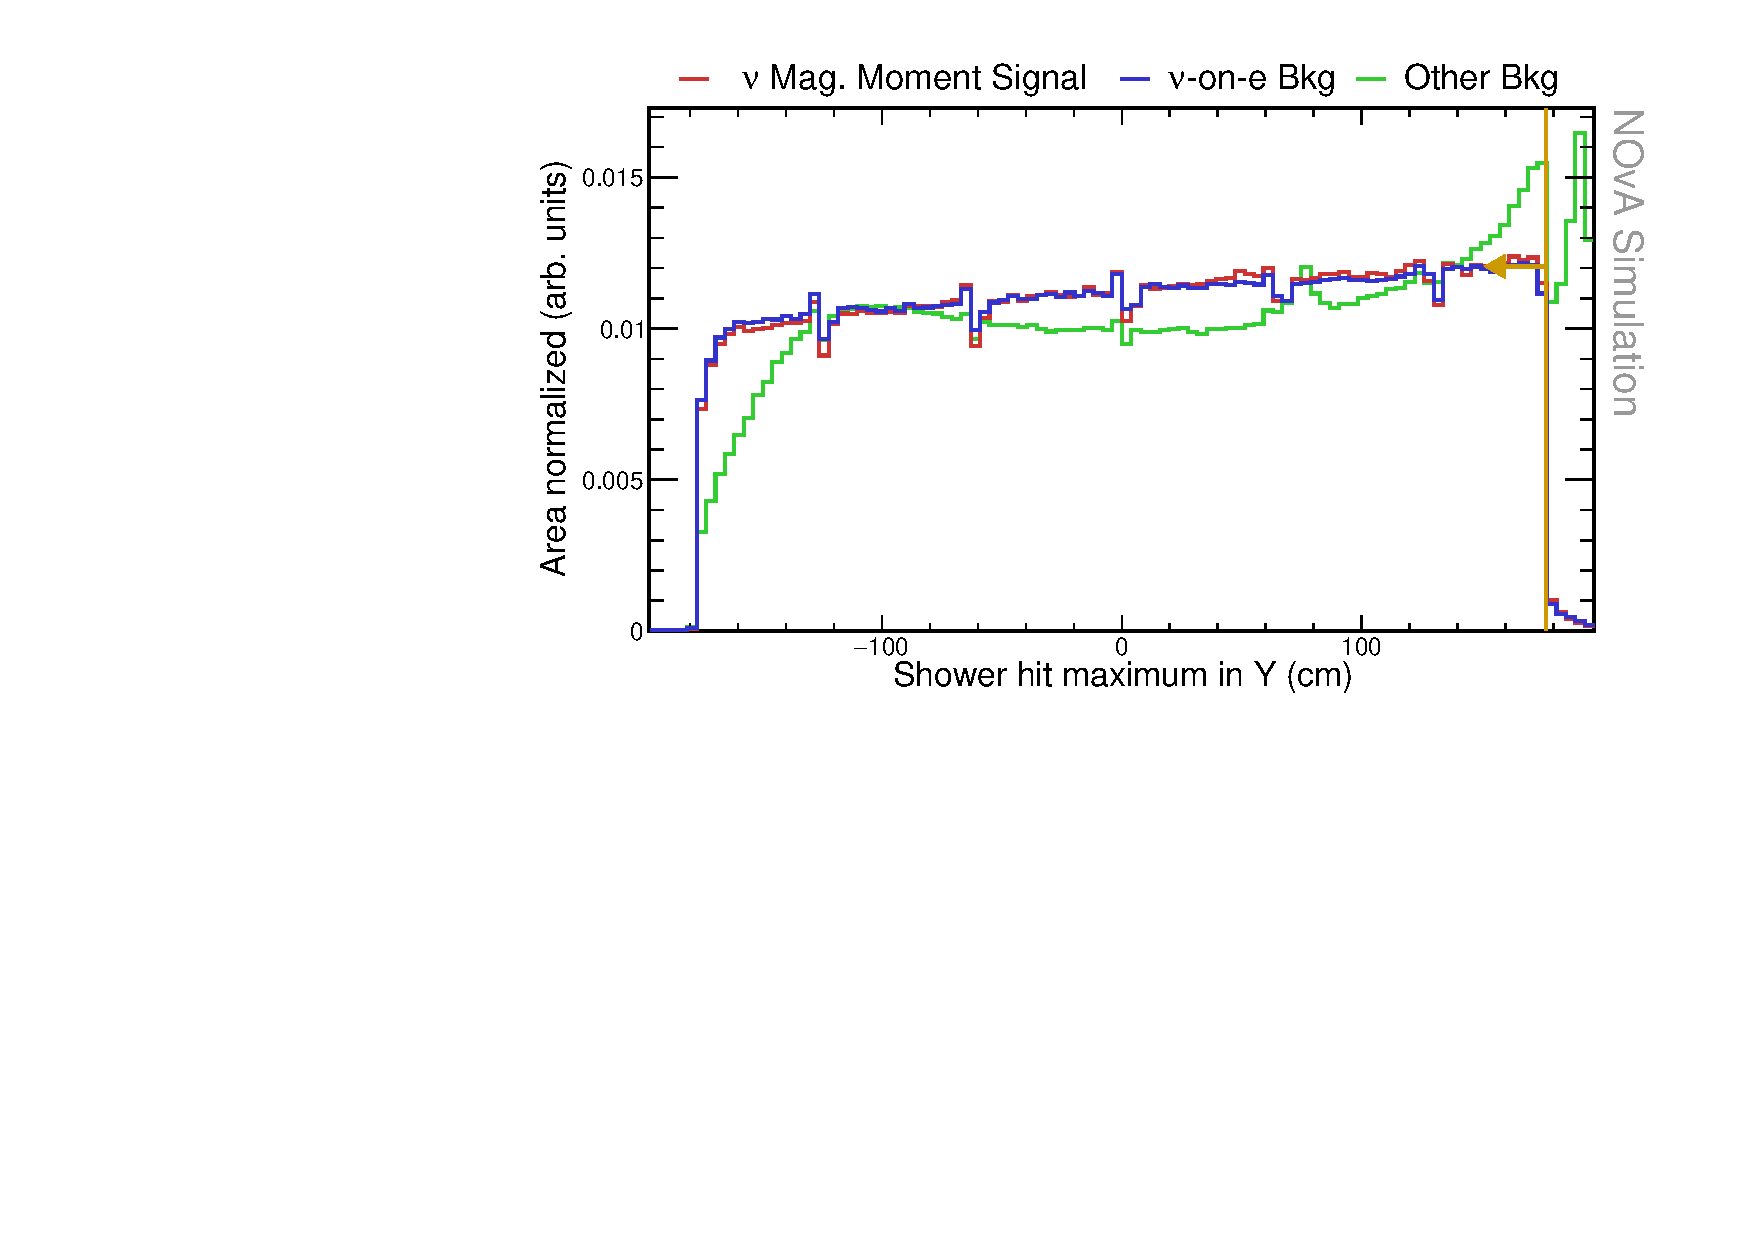
\includegraphics[width=.7\textwidth]{Plots/NuMMEventSelection/N1Cut_maxY.pdf}
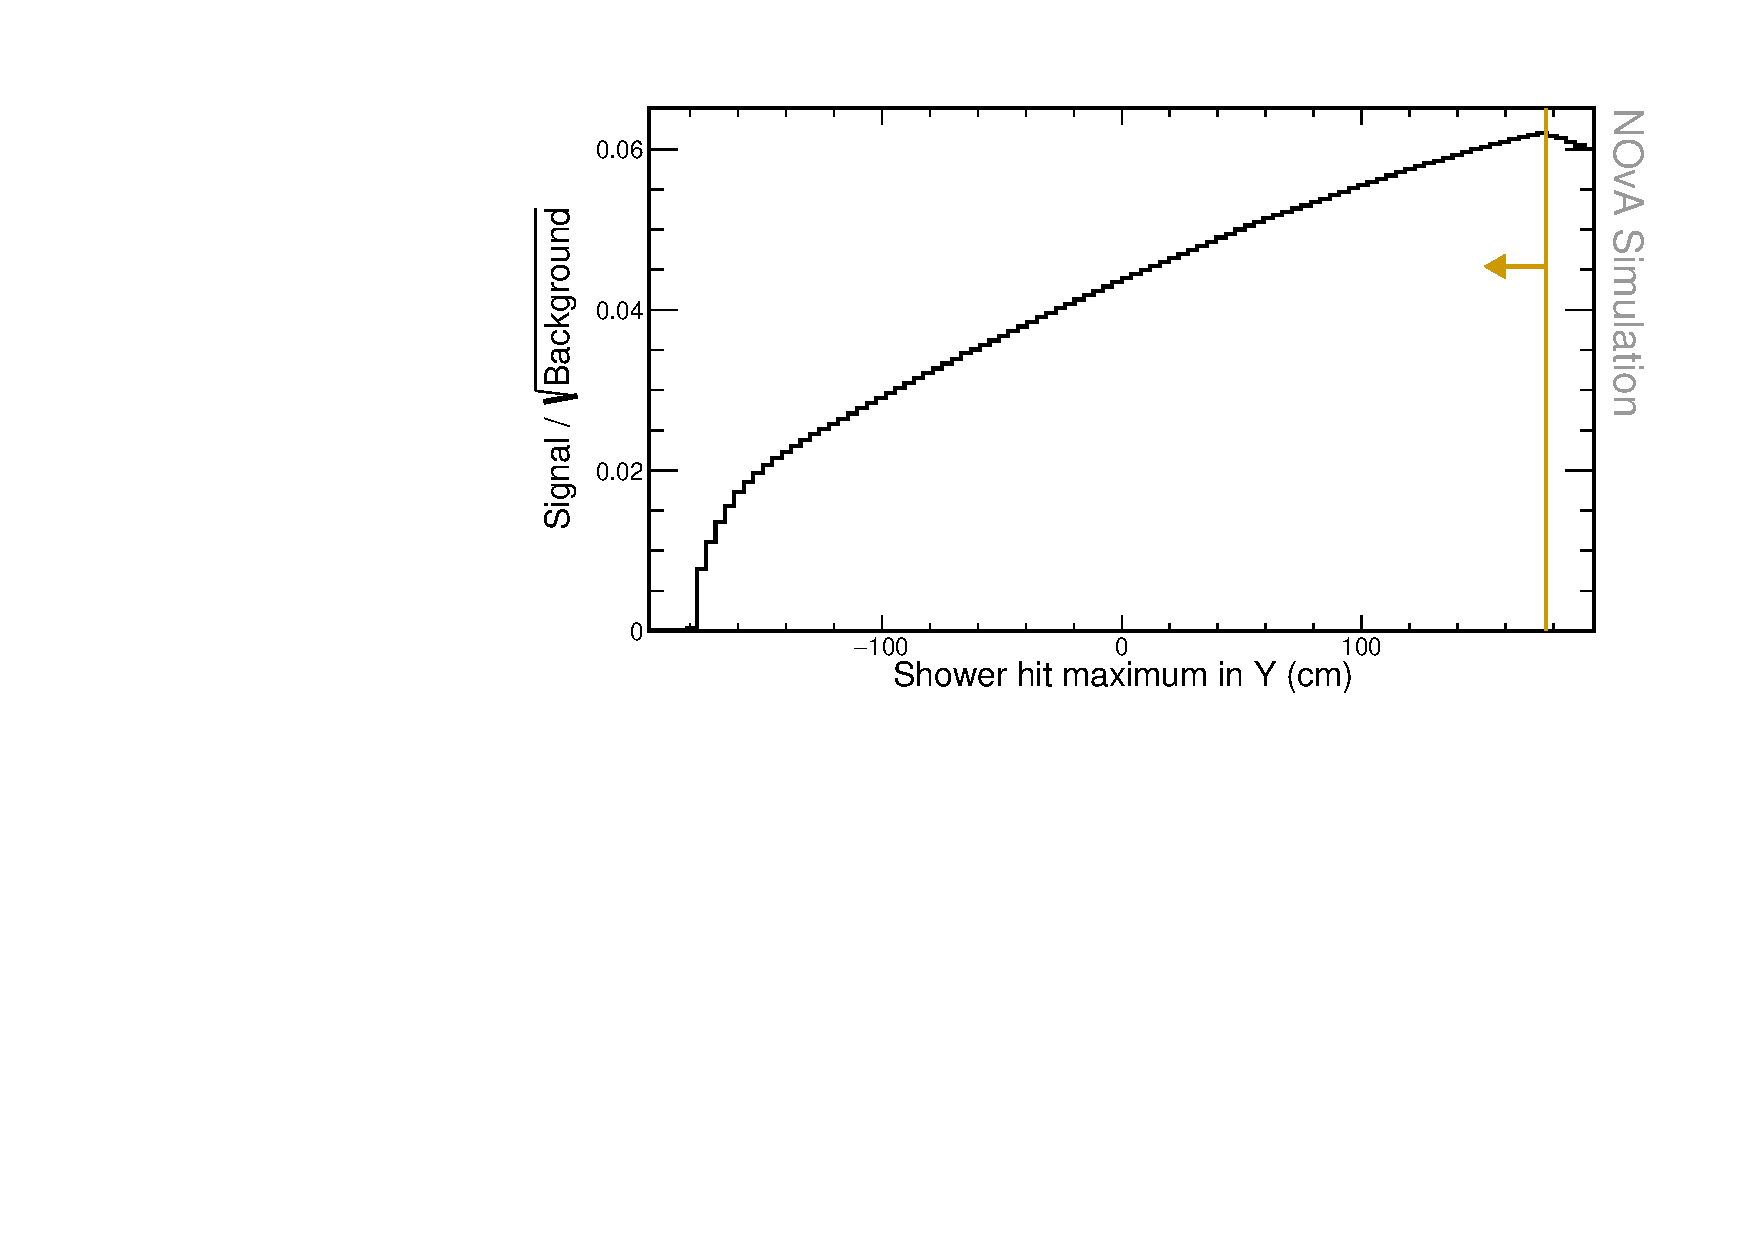
\includegraphics[width=.7\textwidth]{Plots/NuMMEventSelection/NuMM_N1Cut_maxYleft_FOMStats}
\caption[Hit maximum y containment cut]{Top: Relative comparison of signal (red), \acrshort{nuone} background (blue), and other background (green) events in the distribution of the maximum hit position of the most energetic prong along the y axis. All histograms are area-normalized. Bottom: Cumulative \acrshort{FOM} calculated as the number of signal events, divided by the number of background events from that bin until the end of the plot in the direction of the yellow arrow. The reconstruction quality, pre-selection and fiducial cuts were applied prior to making these plots. Yellow lines show the cut values that create the containment volume, with arrows pointing towards the preserved events.}
\label{fig:NuMMContainmentCutMaxY}
\end{figure}

\begin{figure}[hbtp]
\centering
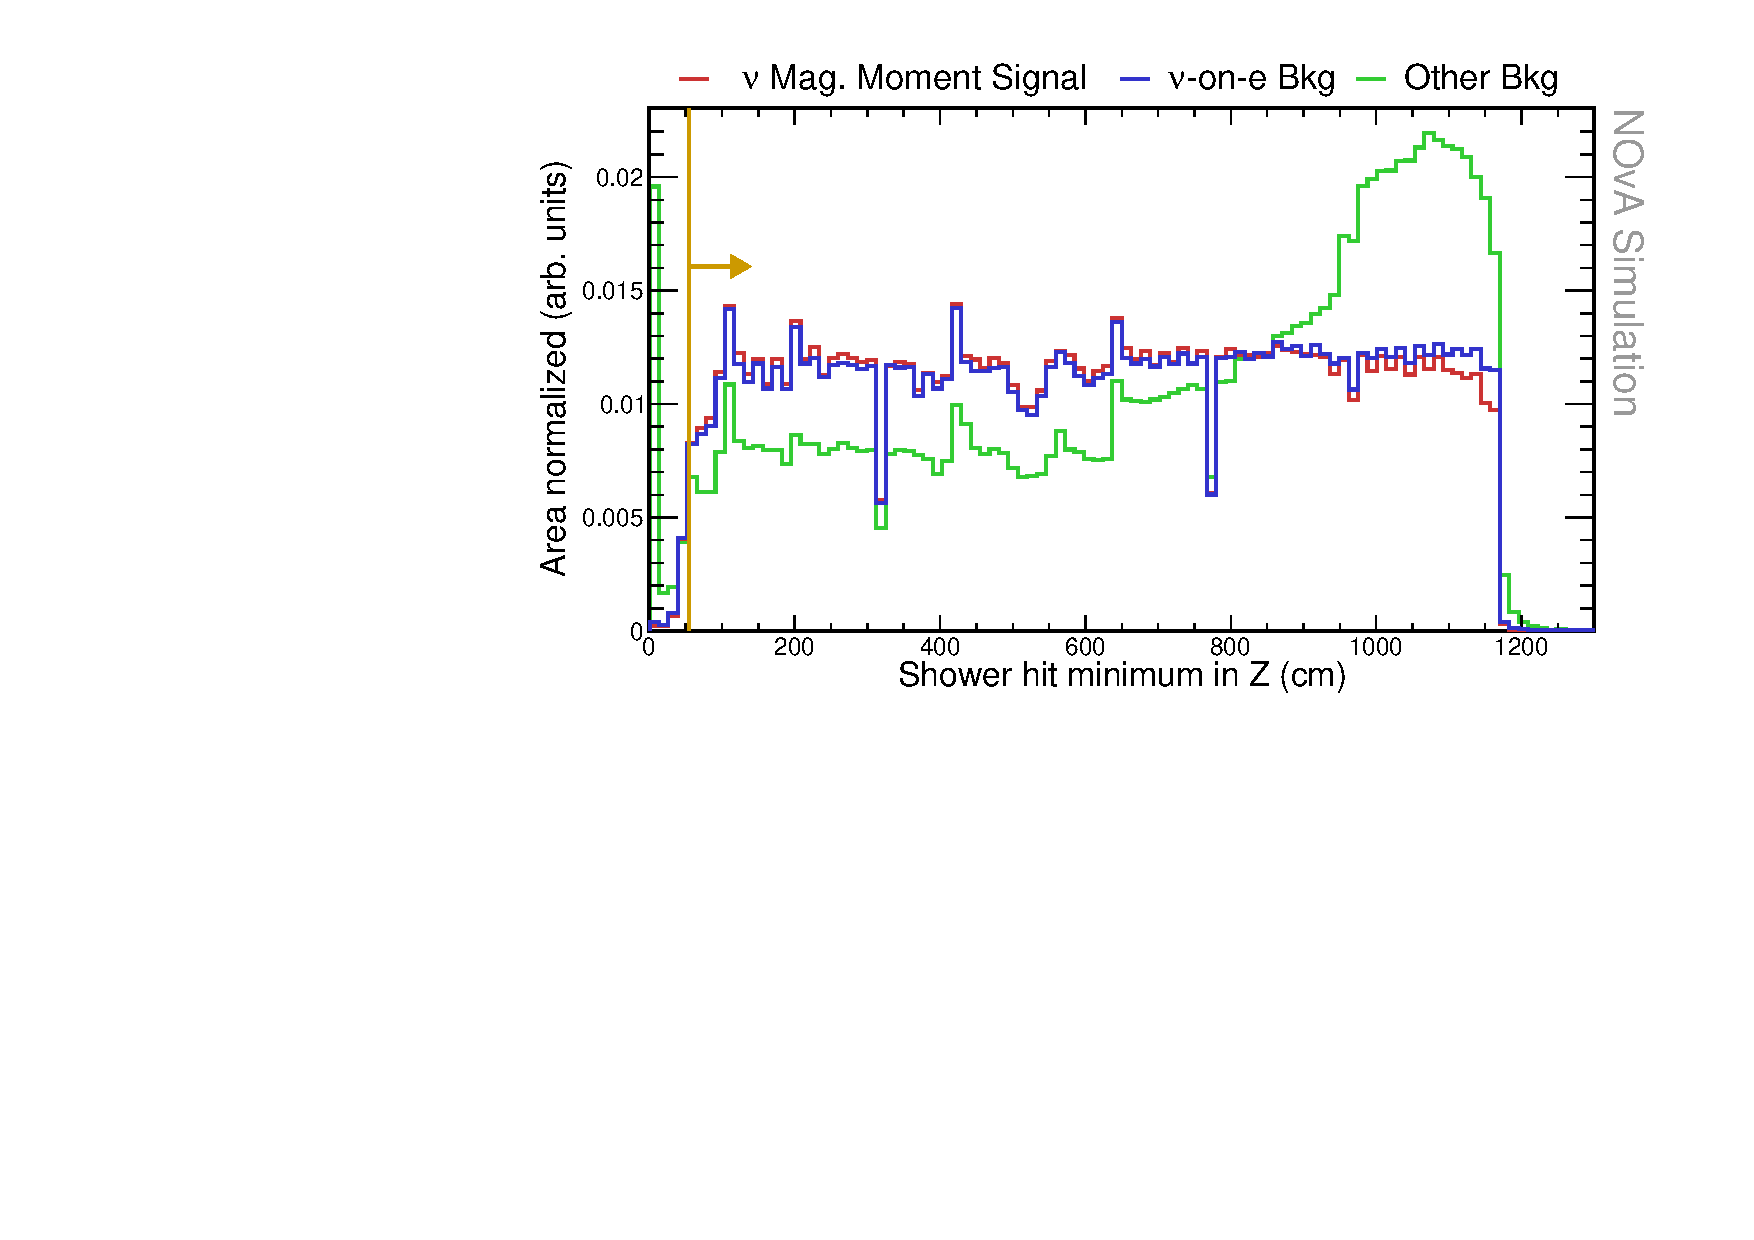
\includegraphics[width=.7\textwidth]{Plots/NuMMEventSelection/N1Cut_minZ.pdf}
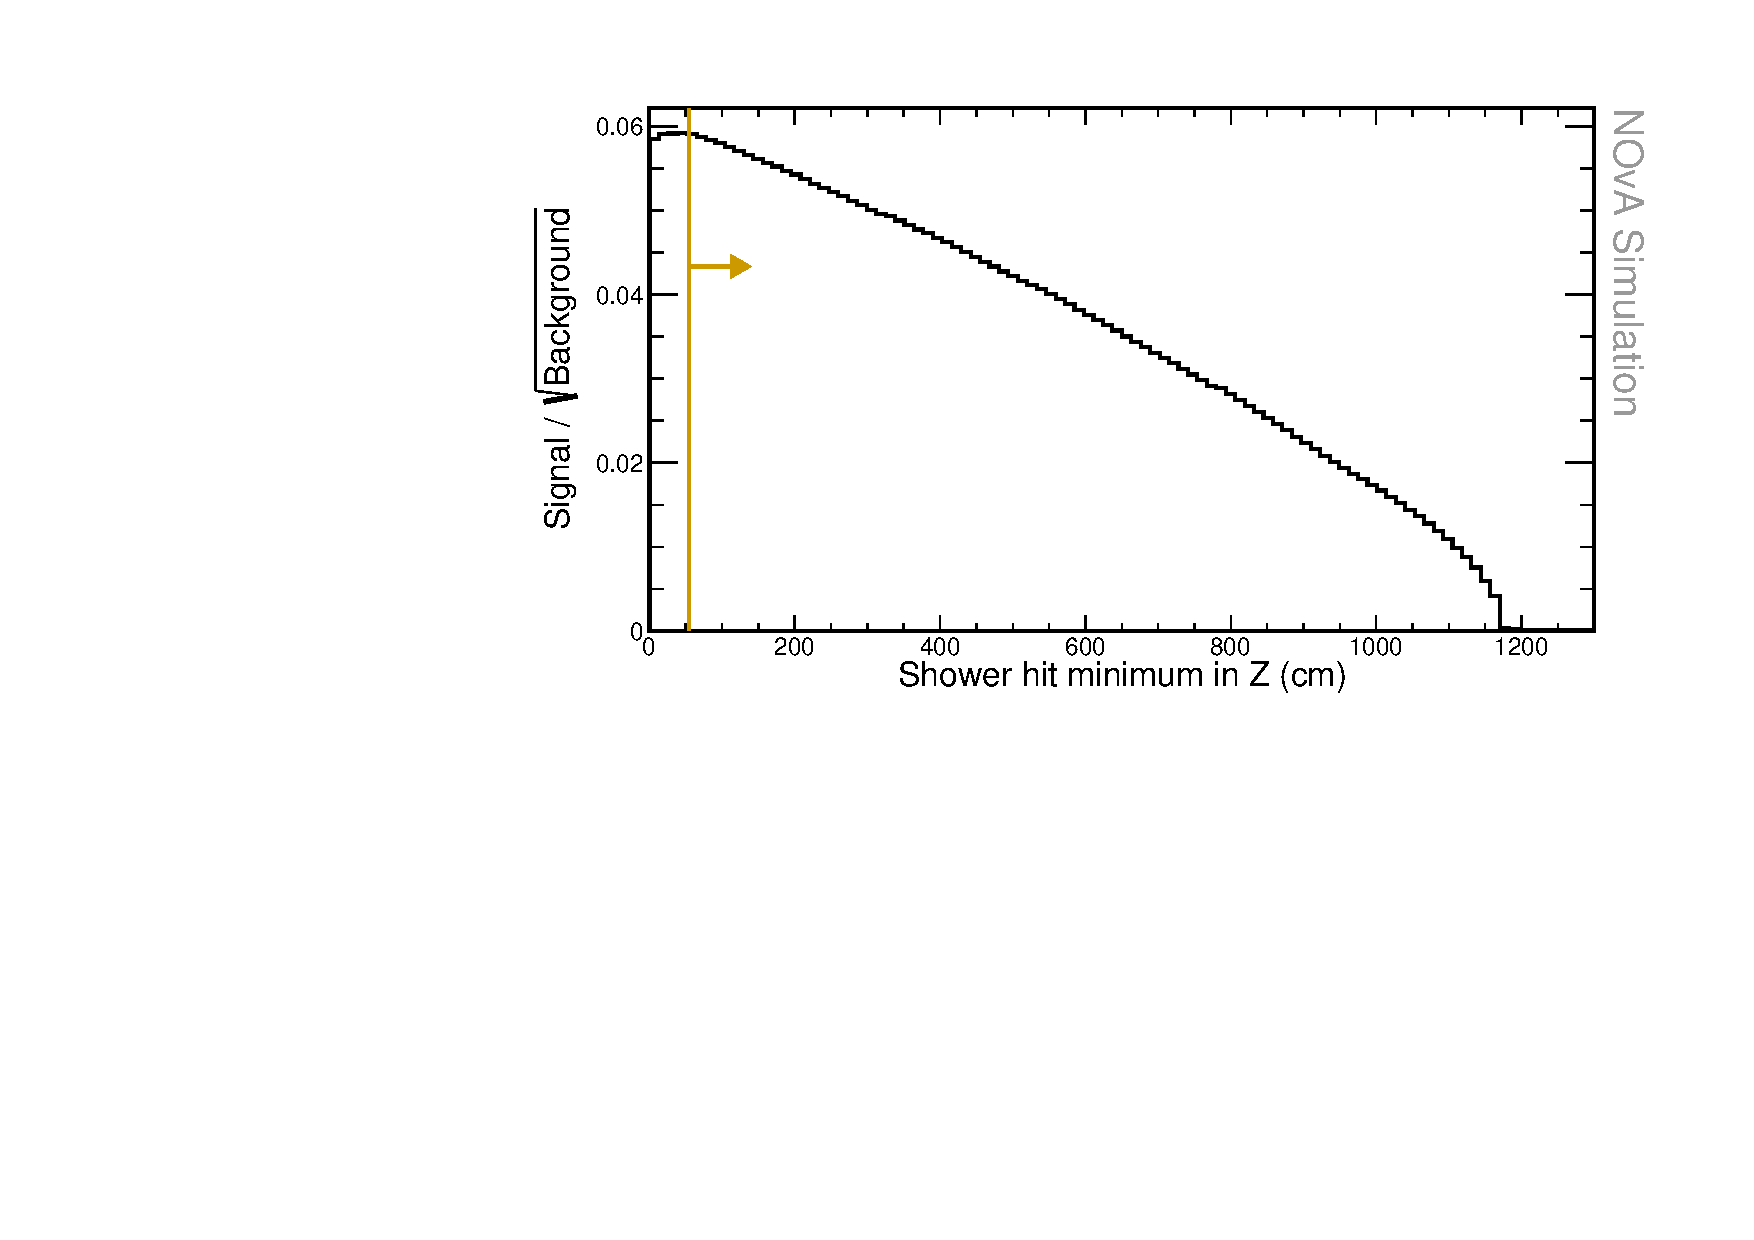
\includegraphics[width=.7\textwidth]{Plots/NuMMEventSelection/NuMM_N1Cut_minZright_FOMStats.pdf}
\caption[Hit minimum z containment cut]{Top: Relative comparison of signal (red), \acrshort{nuone} background (blue), and other background (green) events in the distribution of the minimum hit position of the most energetic prong along the z axis. All histograms are area-normalized. Bottom: Cumulative \acrshort{FOM} calculated as the number of signal events, divided by the number of background events from that bin until the end of the plot in the direction of the yellow arrow. The reconstruction quality, pre-selection and fiducial cuts were applied prior to making these plots. Yellow lines show the cut values that create the containment volume, with arrows pointing towards the preserved events.}
\label{fig:NuMMContainmentCutMinZ}
\end{figure}

\begin{figure}[hbtp]
\centering
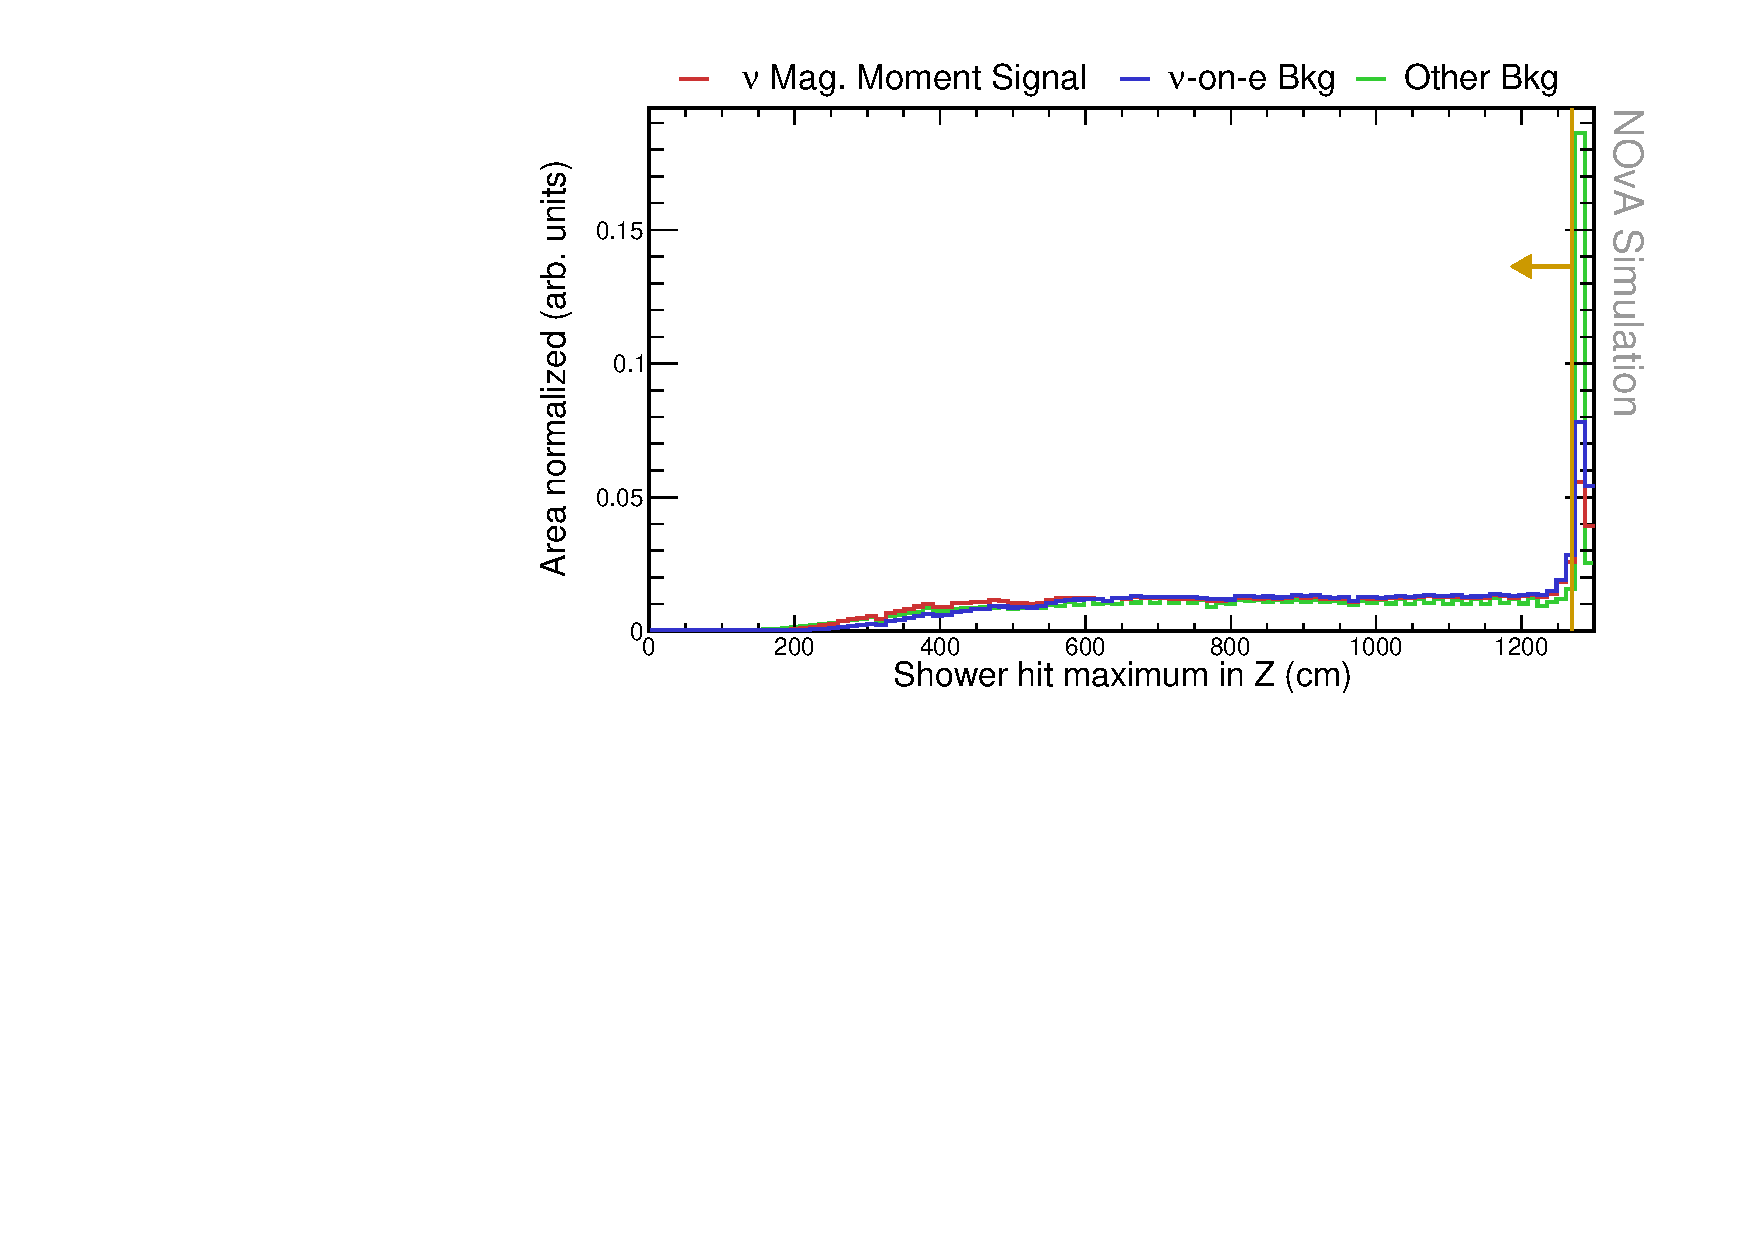
\includegraphics[width=.7\textwidth]{Plots/NuMMEventSelection/N1Cut_maxZ.pdf}
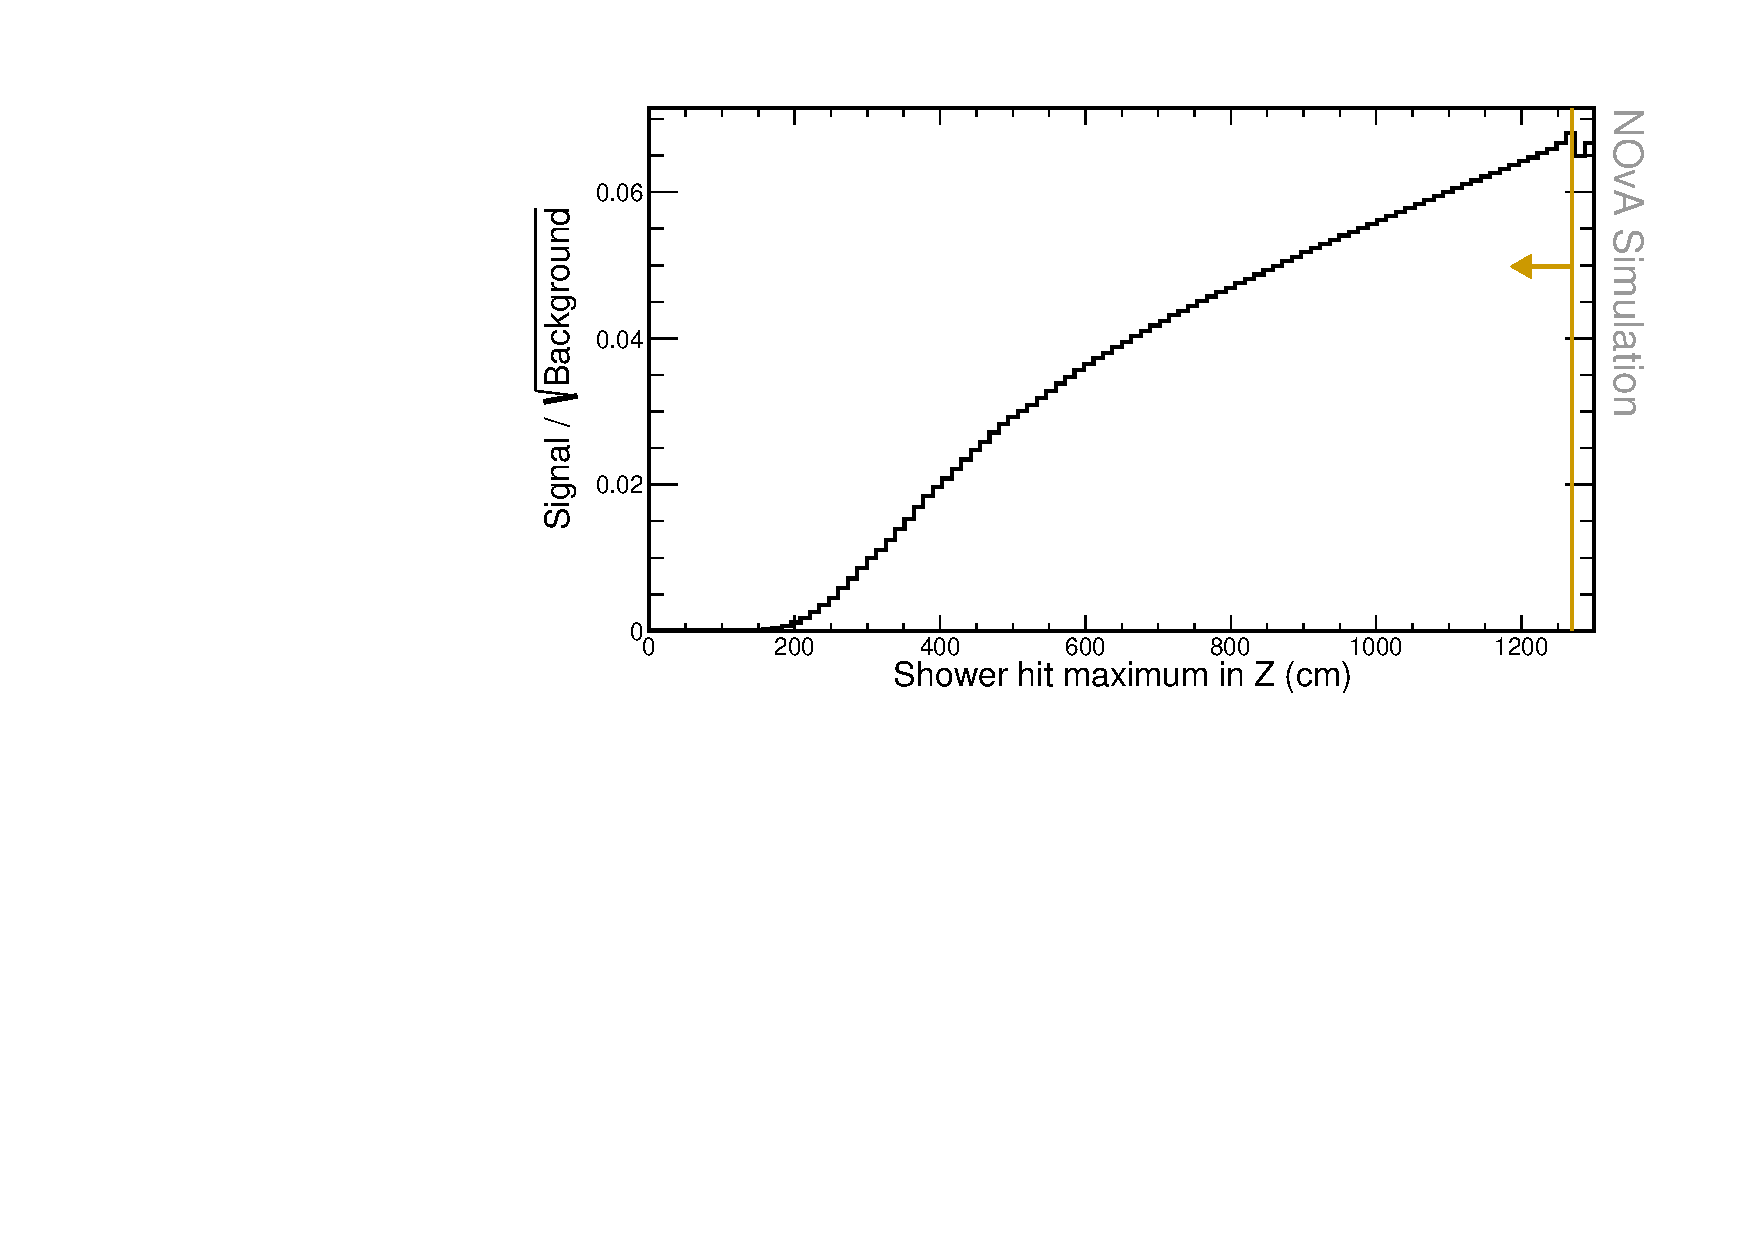
\includegraphics[width=.7\textwidth]{Plots/NuMMEventSelection/NuMM_N1Cut_maxZleft_FOMStats}
\caption[Hit maximum z containment cut]{Top: Relative comparison of signal (red), \acrshort{nuone} background (blue), and other background (green) events in the distribution of the maximum hit position of the most energetic prong along the z axis. All histograms are area-normalized. Bottom: Cumulative \acrshort{FOM} calculated as the number of signal events, divided by the number of background events from that bin until the end of the plot in the direction of the yellow arrow. The reconstruction quality, pre-selection and fiducial cuts were applied prior to making these plots. Yellow lines show the cut values that create the containment volume, with arrows pointing towards the preserved events.}
\label{fig:NuMMContainmentCutMaxZ}
\end{figure}

\begin{table}[!hb]
\centering
\caption[Event selection cutflow table for the containment cuts]{Event selection cutflow table for the containment cuts showing the number of events and the relative efficiency of each cut for each signal sample. The relative efficiency is calculated as number of events remaining after applying the corresponding cut divided by number of event for all the previous cuts. All the cuts are listed in sequence as they are applied. The top row corresponds to the sample after applying the reconstruction quality and pre-selection cuts.}
\begin{tabular}{|l|cc|cc|cc|}\hline
\multicolumn{1}{|c|}{} & \multicolumn{2}{c|}{\textbf{Signal}} & \multicolumn{2}{c|}{\textbf{$\nu$-on-e bkg}} & \multicolumn{2}{c|}{\textbf{Other bkg}} \\
\multicolumn{1}{|c|}{\multirow{-2}{*}{\textbf{Selection}}} & \textbf{$N_{evt}$} & \textbf{$\epsilon_{rel}\left(\%\right)$} & \textbf{$N_{evt}$} & \textbf{$\epsilon_{rel}\left(\%\right)$}  & \textbf{$N_{evt}$} & \textbf{$\epsilon_{rel}\left(\%\right)$}\\\hline
\textbf{Pre-selection} & 155.14 & 100 & 3.33$\times 10^3$ & 100 & 8.83$\times 10^6$ & 100\\
\textbf{Fiducial} & 143.02 & 92.19 & 2.88$\times 10^3$ & 85.60 & 5.96$\times 10^6$ & 67.57\\
\textbf{Containment} & 117.41 & 82.09 & 2.08$\times 10^3$ & 72.12 & 1.10$\times 10^6$ & 18.38\\\hline
\end{tabular}
\label{tab:CutflowTableFiducialContainmnet}
\end{table}

\subsection{Multivariate analysis}\label{sec:NuMMEventSelTMVA}
%%% TMVA
Following the removal of obvious backgrounds and events not contained within the detector, we aim to optimise the event selection to achieve the highest significance for measuring the effective muon neutrino magnetic moment. This goal is equivalent to maximising our \gls{FOM} from Eq.~\ref{eq:NuMMFOM}.

For this purpose, we utilised ROOT's \cite{ROOT} \gls{TMVA} \cite{TMVA}. Specifically, we employed the rectangular cut optimisation method, which uses multivariate parameter fitters to maximise background rejection across the full range of signal efficiencies. We used the \gls{MC} sampling fitting method, assuming that for each input variable, there is a single cut value (maximum or minimum) that optimally discriminates between signal and background.

%Specifically, we are doing this to the inputs, using this number of inputs, these transformations, this algorithms, this distribution of signal and background events with this specific splits, and this number of signal and background events for the evaluation.

%The optimisation of cuts performed by TMVA maximises the background rejection at given signal efficiency, and scans over the full range of the latter quantity. TMVA cut optimisation is performed with the use of multivariate parameter fitters, specifically with the Monte Carlo sampling for us. All optimisation methods (fitters) act on the assumption that one minimum and one maximum requirement on each variable is sufficient to optimally discriminate signal from background (i.e., the signal is clustered). Since I used the fSmart option, my vars are required to have a dedicated min OR max. 

%%%Input variables
\gls{TMVA} generally performs better with a limited number of input variables that have strong discriminating power. Therefore, we investigated several input variables and selected only those that achieved significant background rejection. There are additional variables not mentioned here that might achieve better final results, providing opportunities for future re-analyses. Additionally, we do not apply any transformations to the input variables prior to optimisation, which might also improve the final result after dedicated study.

The variables considered include those already used in the pre-selection: the total number of hits for all prongs in slice, the length of the longest prong, and $E\theta^2$, as discussed in Sec.~\ref{sec:NuMMEventSelectionPresel}. During the \gls{TMVA} optimisation, we found that the length of the longest prong did not significantly enhance discriminating power and thus removed it from the set of input variables. Additionally, we included the reconstructed energy of the most energetic shower, as used for reconstruction quality selection in Sec.~\ref{sec:NuMMEventSelRecoQC}, intending to restrict events with higher energies, since our signal is concentrated at low electron recoil energies.

Additionally, we considered all the variables used for the \gls{NOvA} \gls{nuone} analysis for the neutrino flux constraint \cite{NOVA-doc-56383}. The first is the fraction of the reconstructed energy of the most energetic shower $\left(E_{Shower}\right)$ to the total energy of all the reconstructed prongs in the entire slice $\left(E_{Tot}\right)$. This variable distinguished our signal events, which only have a single shower, from events with multiple showers or additional activity. The second is the gap between the vertex and the most energetic shower, which can distinguish between electron and $\pi^0$ events, as the latter should have a characteristic gap several cells long. Additionally, we examined the amount of energy contained within $\pm8$ planes away from the vertex, besides the energy associated with the most energetic prong, which should distinguish the purely leptonic signal from backgrounds with significant hadronic activity. However, the gap and the vertex energy variables underperformed compared to others and were ultimately not used within the \gls{TMVA}.

We also utilised two \gls{CNN}-based event classifiers developed by the \gls{ND} group for the \gls{NOvA} \gls{nuone} analysis for the neutrino flux constraint \cite{NOVA-doc-56383}. These classifiers are specifically designed to identify \gls{nuone} interactions. The first, named \gls{nuone}\texttt{ID}, is trained to select \gls{nuone} events from the primary $\nu_\mu$\gls{CC} background, while the second, named $E\pi^0$\texttt{ID}, is trained on events passing the \gls{nuone}\texttt{ID} selection to reject the remaining background with a $\pi^0$. These classifiers use a pixel map of the entire slice as input and are designed with the same \gls{CNN} architecture as ProngCVN and EventCVN.

%[ND group's technote] Two event classifiers (NuoneID and Epi0ID) based on convolutional neural network (CNN) are trained to identify nuone elastic scattering events (NuoneID) and to further reject background with pi0 in the final state (Epi0ID). The CNN architecture adopted for this analysis is the one used for NOvA CVN [12]. It takes the pixel map of a slice as the input and has deeper and more complicated neural networks than the ANNs used in the previous round of analysis [11]. The training for both classifiers (NuoneID and Epi0ID) were done with single electron samples as the signal in order to mitigate the model dependence. A nuone elastic scattering has an electron in the final state which could deposit energy in the detector. Single electron events share this feature with nuone elastic scattering, but have more uniform distribution of energy, angle between the shower direction and the beam direction. This additional feature could prevent CNN models from overfitting the feature of the very small scattering angle.  To make comparisons, test samples of signal and background are normalized to 1.1E21. The output categories are \gls{nuone}, $\pi^0$, $\nu_e$\gls{CC} and other. The \gls{nuone} and $\pi^0$ outputs are used for the training of the Epi0ID. The pre-selection applied is: ND group's preselection ($L<\unit[800]{cm}$, $N_{plane}<120$, $N_{cell}<600$), loose containment ($-190<X<190$, $-190<Y<190$, $50<Z<1500$ $\unit{cm}$), loose single particle cut ($E_{vtx}<\unit[0.05]{GeV}$, $gap<\unit[20]{cm}$, $E_{shower}/E_{tot} > 0.9$ \note{These are quite strict actually}. The training accuracy for NuoneID is about 85\% and for Epi0ID is about 96\%. After each round of training, the trained model is saved to make predictions on the test sample so we know how the actual performance of the classifiers evolves over different epochs.

%%% Result
The result of the \gls{TMVA} is a set of cuts on each of the input variables that maximises the \gls{FOM}. The input variables and the cuts that were selected for them are shown in Fig.~\ref{fig:NuMMCutsTMVA1}, \ref{fig:NuMMCutsTMVA2}, and \ref{fig:NuMMCutsTMVA3}. The effect of these cuts is summarised in Tab.~\ref{tab:CutflowTableTMVA}. Applying the \gls{TMVA} cuts reduces the signal by $\unit[51.62]{\%}$, the \gls{nuone} background by $\unit[75.03]{\%}$ and other background by $\unit[99.98]{\%}$. The specific values of the cuts resulting from the \gls{TMVA} are
\begin{align}
E_{Shower}/E_{Tot} &> 0.91,\\
\textsf{Total N}^o\textsf{ hits for all prongs} &< 116,\\
E_{Shower} &< \unit[1.4]{GeV},\\
E\theta^2 &< \unit[0.0048]{GeV\times rad^2},\\
\gls{nuone}\textsf{ID} &> 0.65,\\
E\pi^0\textsf{ID} &> 0.63.
\end{align}

\begin{figure}[hbtp]
\centering
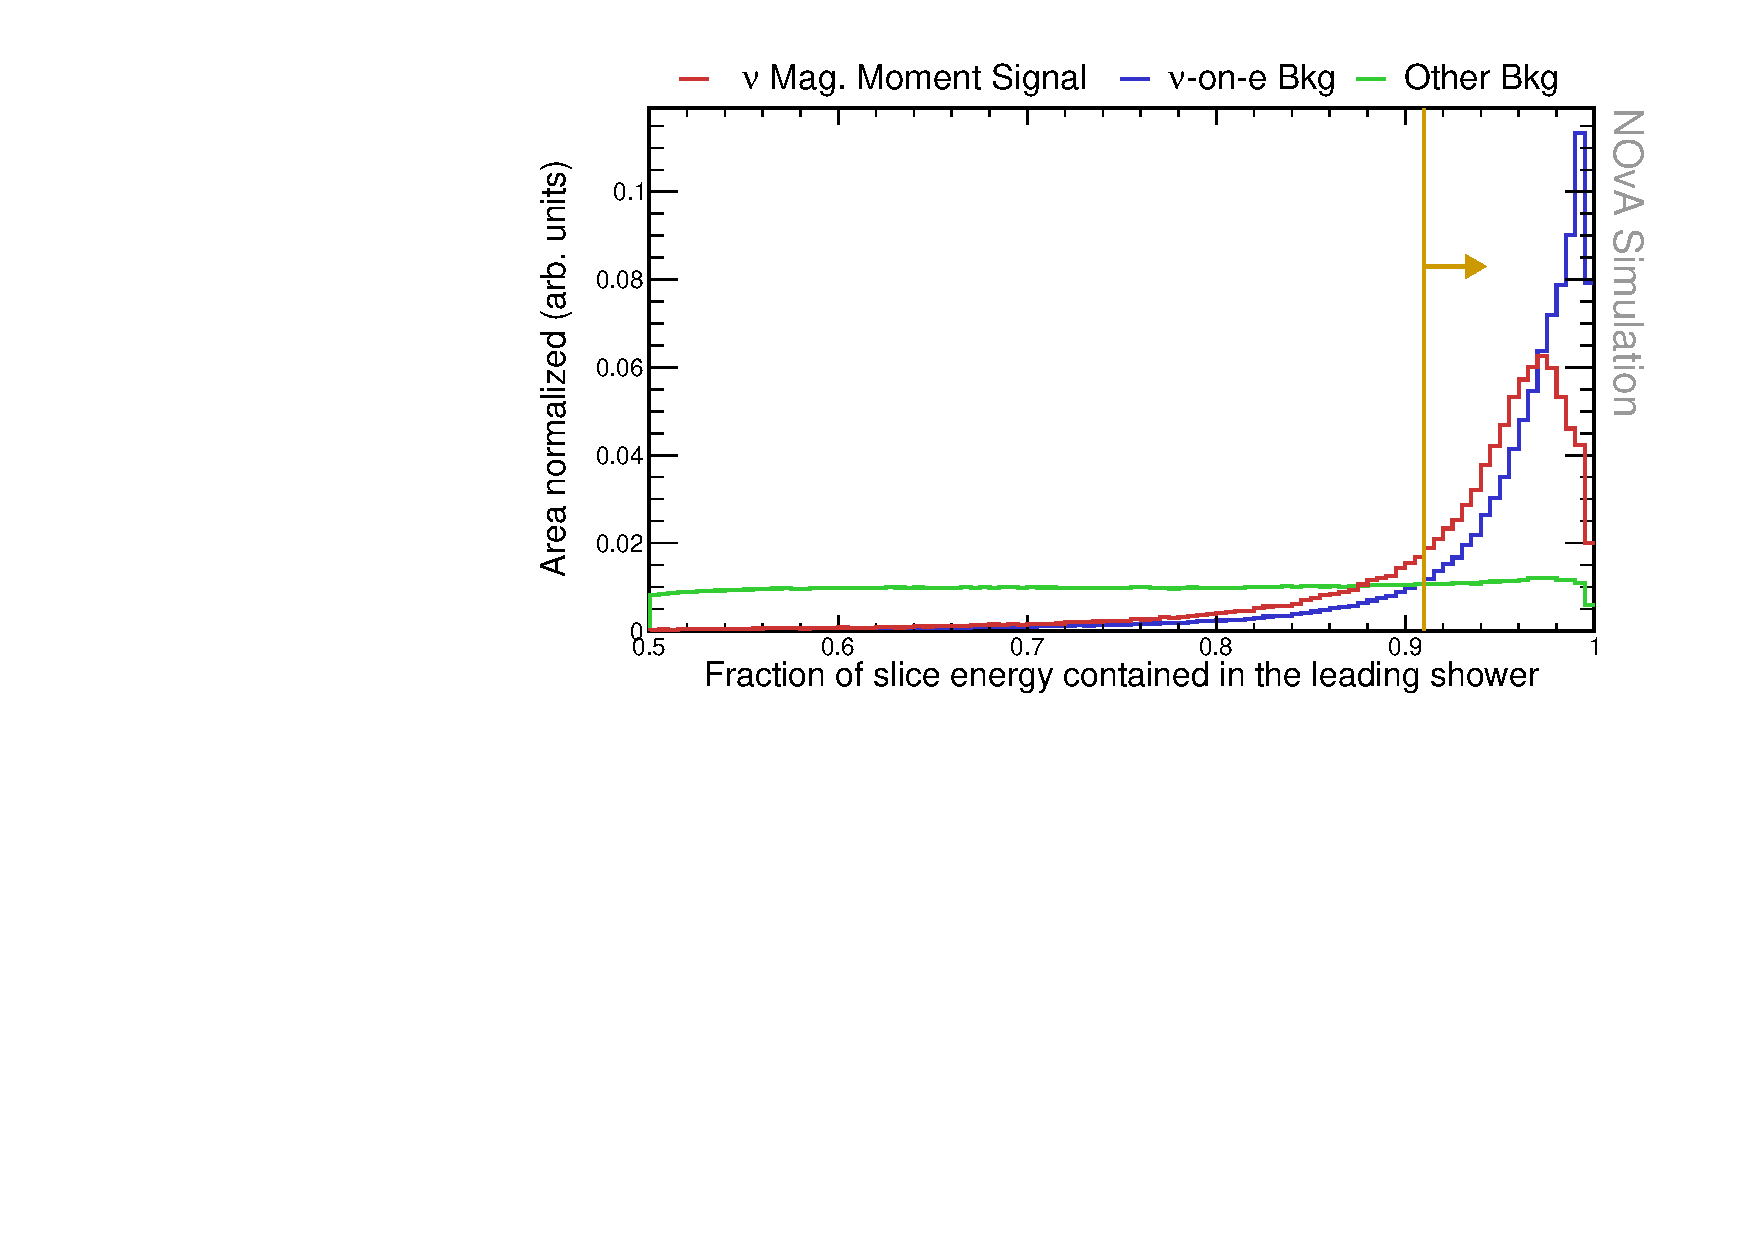
\includegraphics[width=.7\textwidth]{Plots/NuMMEventSelection/N1Cut_shwEFrac.pdf}
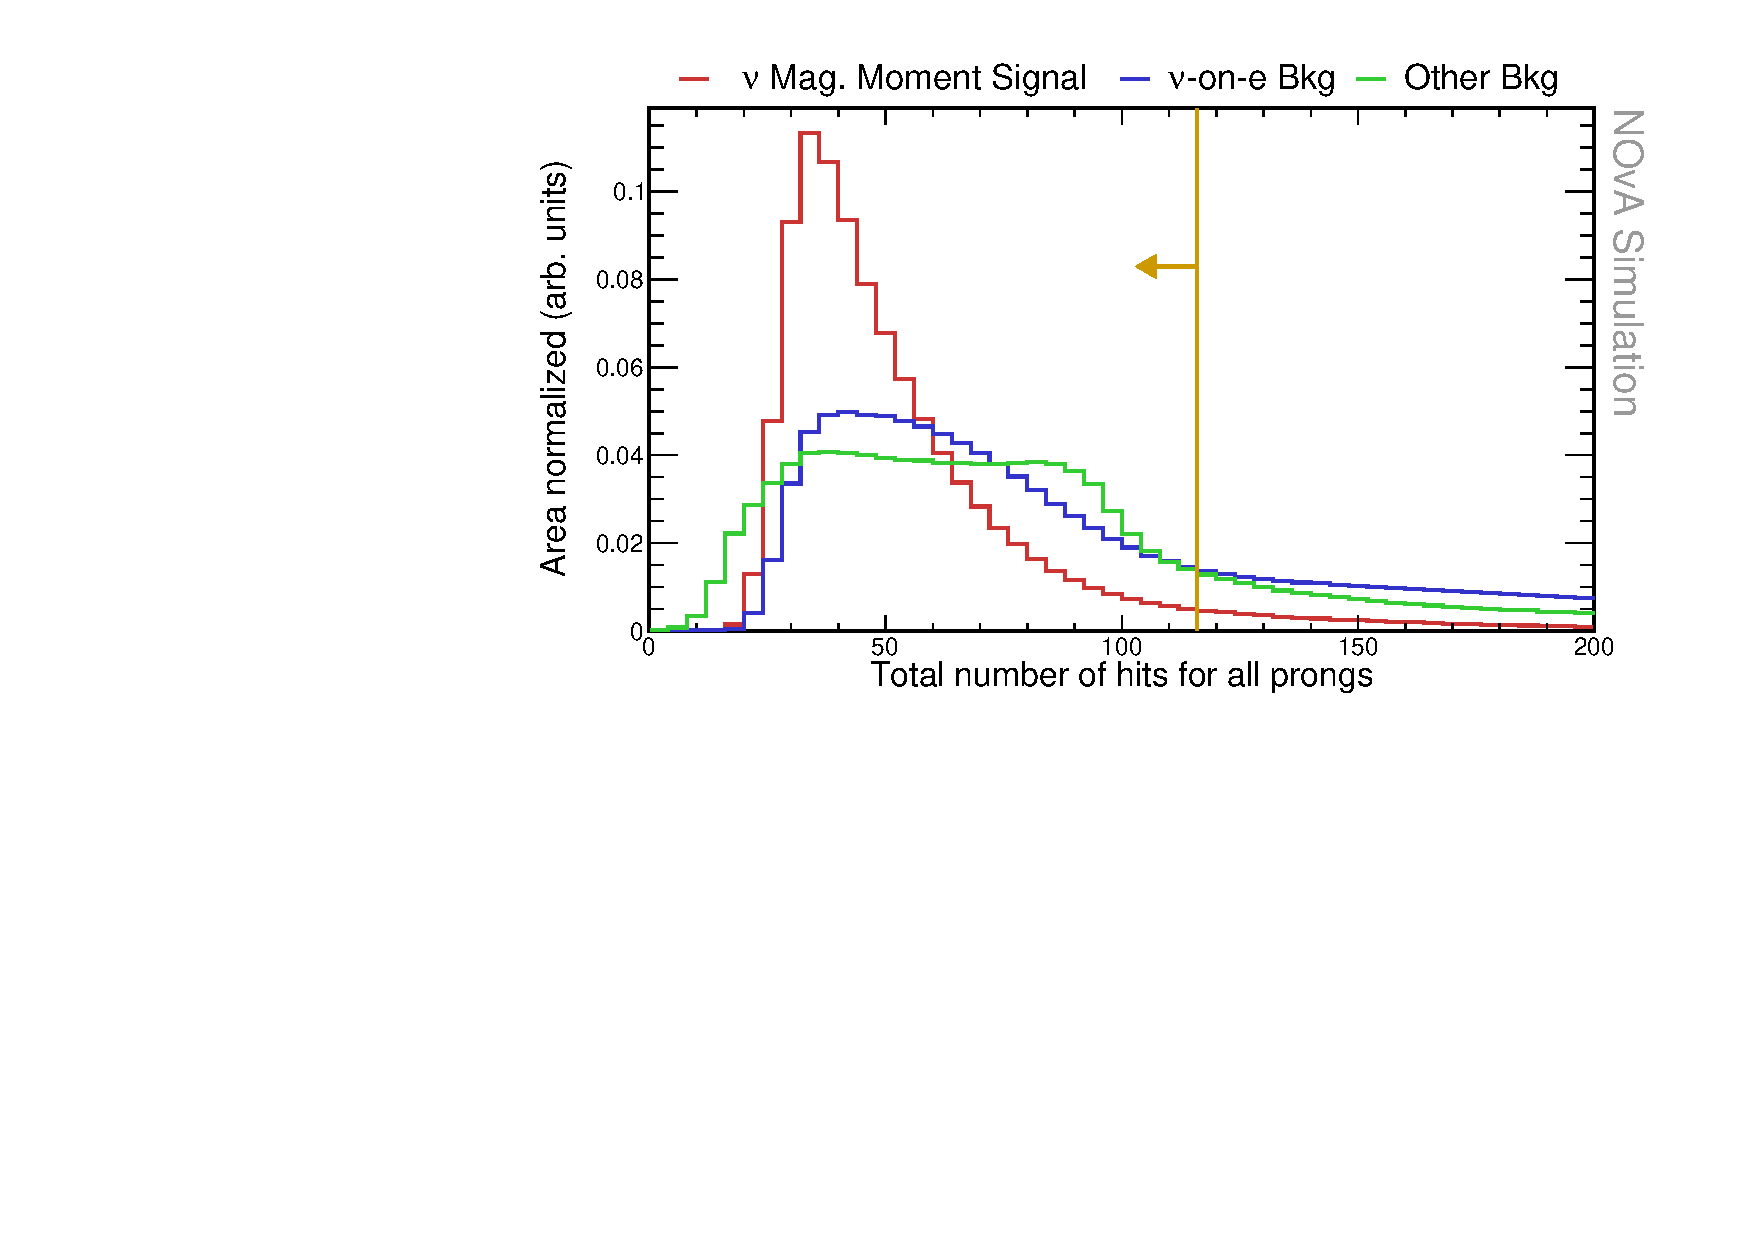
\includegraphics[width=.7\textwidth]{Plots/NuMMEventSelection/N1Cut_NHitsPre.pdf}
\caption[Shower E fraction and number of hits cuts]{Relative comparison of signal (red), \acrshort{nuone} background (blue), and other background (green) events in the distribution of the fraction of the total energy contained in the primary shower (top) and of the total number of hits in the slice (bottom). All histograms are area-normalized. The reconstruction quality, pre-selection, fiducial and containment cuts were applied prior to making these plots. Yellow lines show the cut values on the depicted variables, with arrows pointing towards the preserved events.}
\label{fig:NuMMCutsTMVA1}
\end{figure}

\begin{figure}[hbtp]
\centering
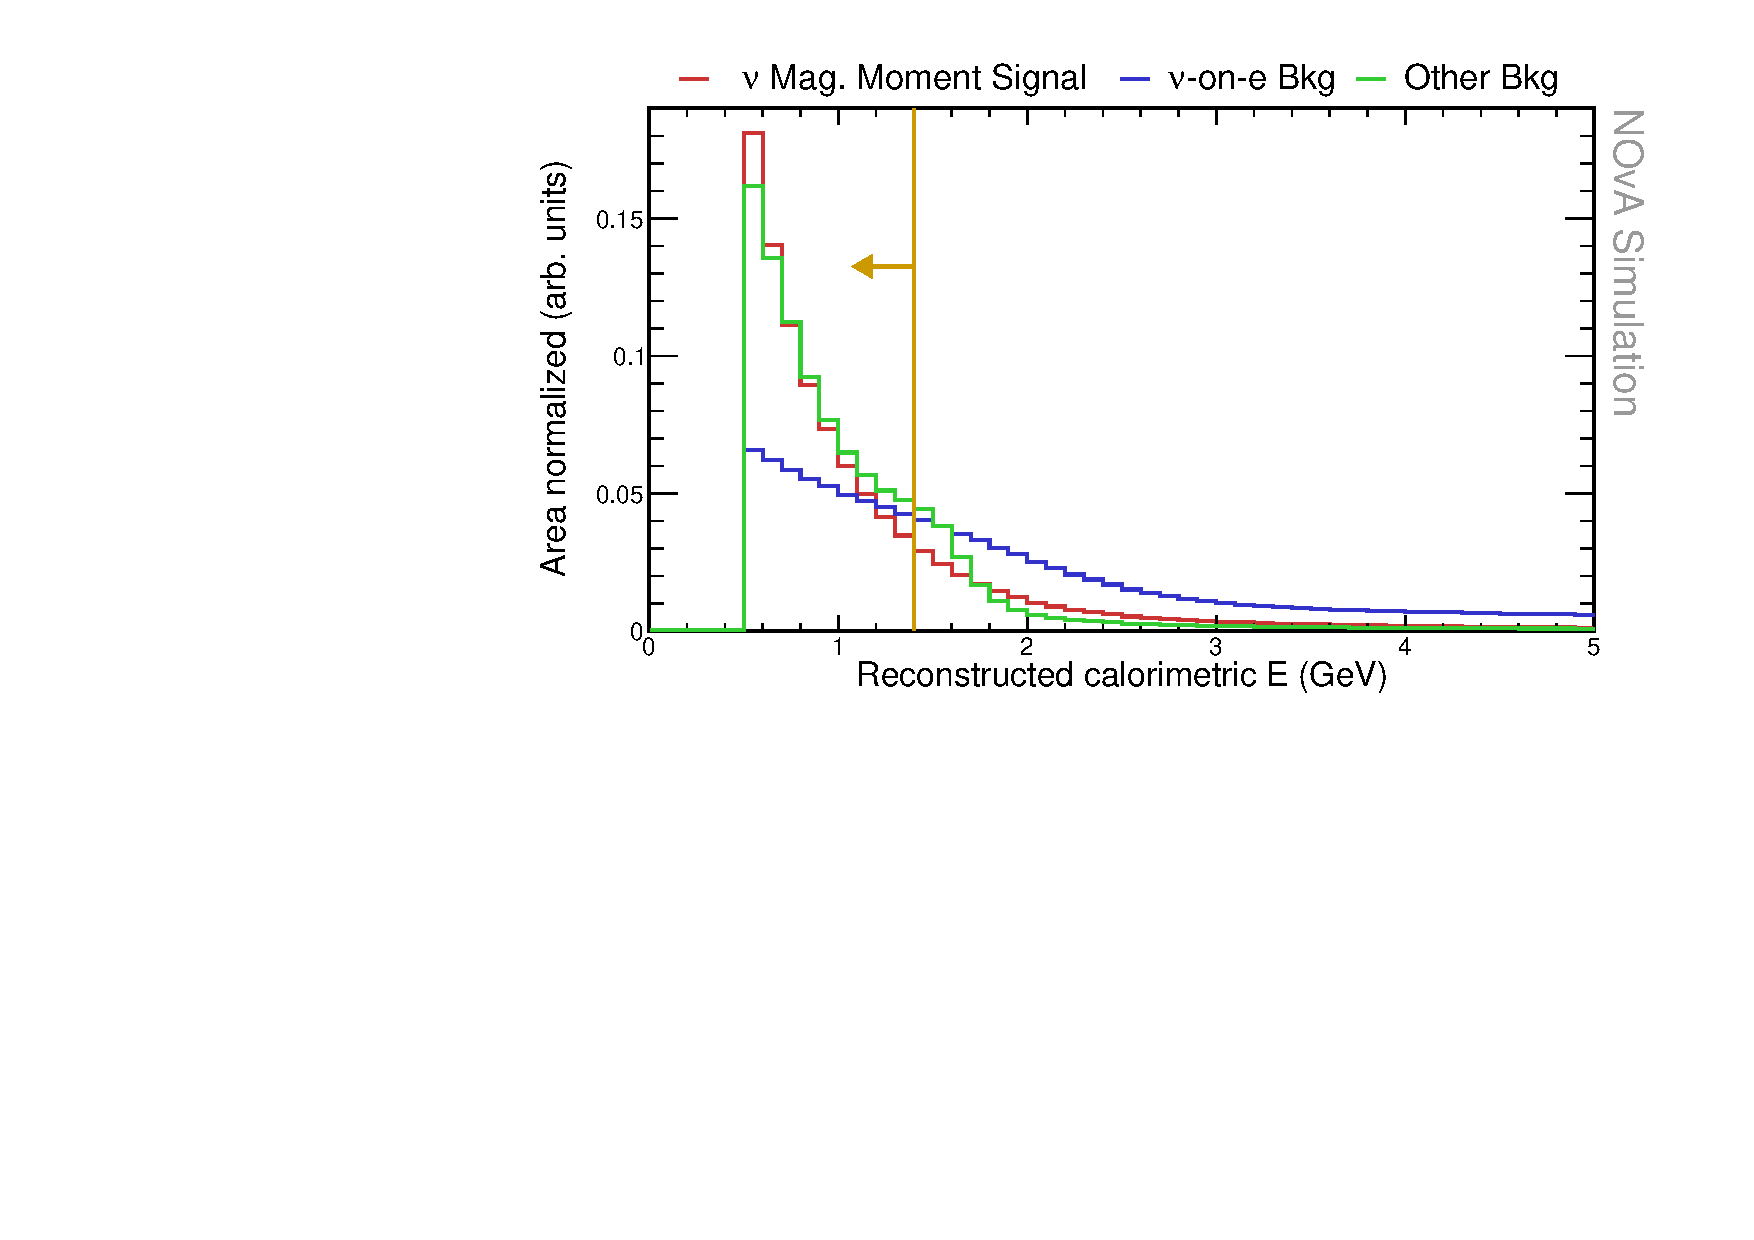
\includegraphics[width=.7\textwidth]{Plots/NuMMEventSelection/N1Cut_calEHighPre.pdf}
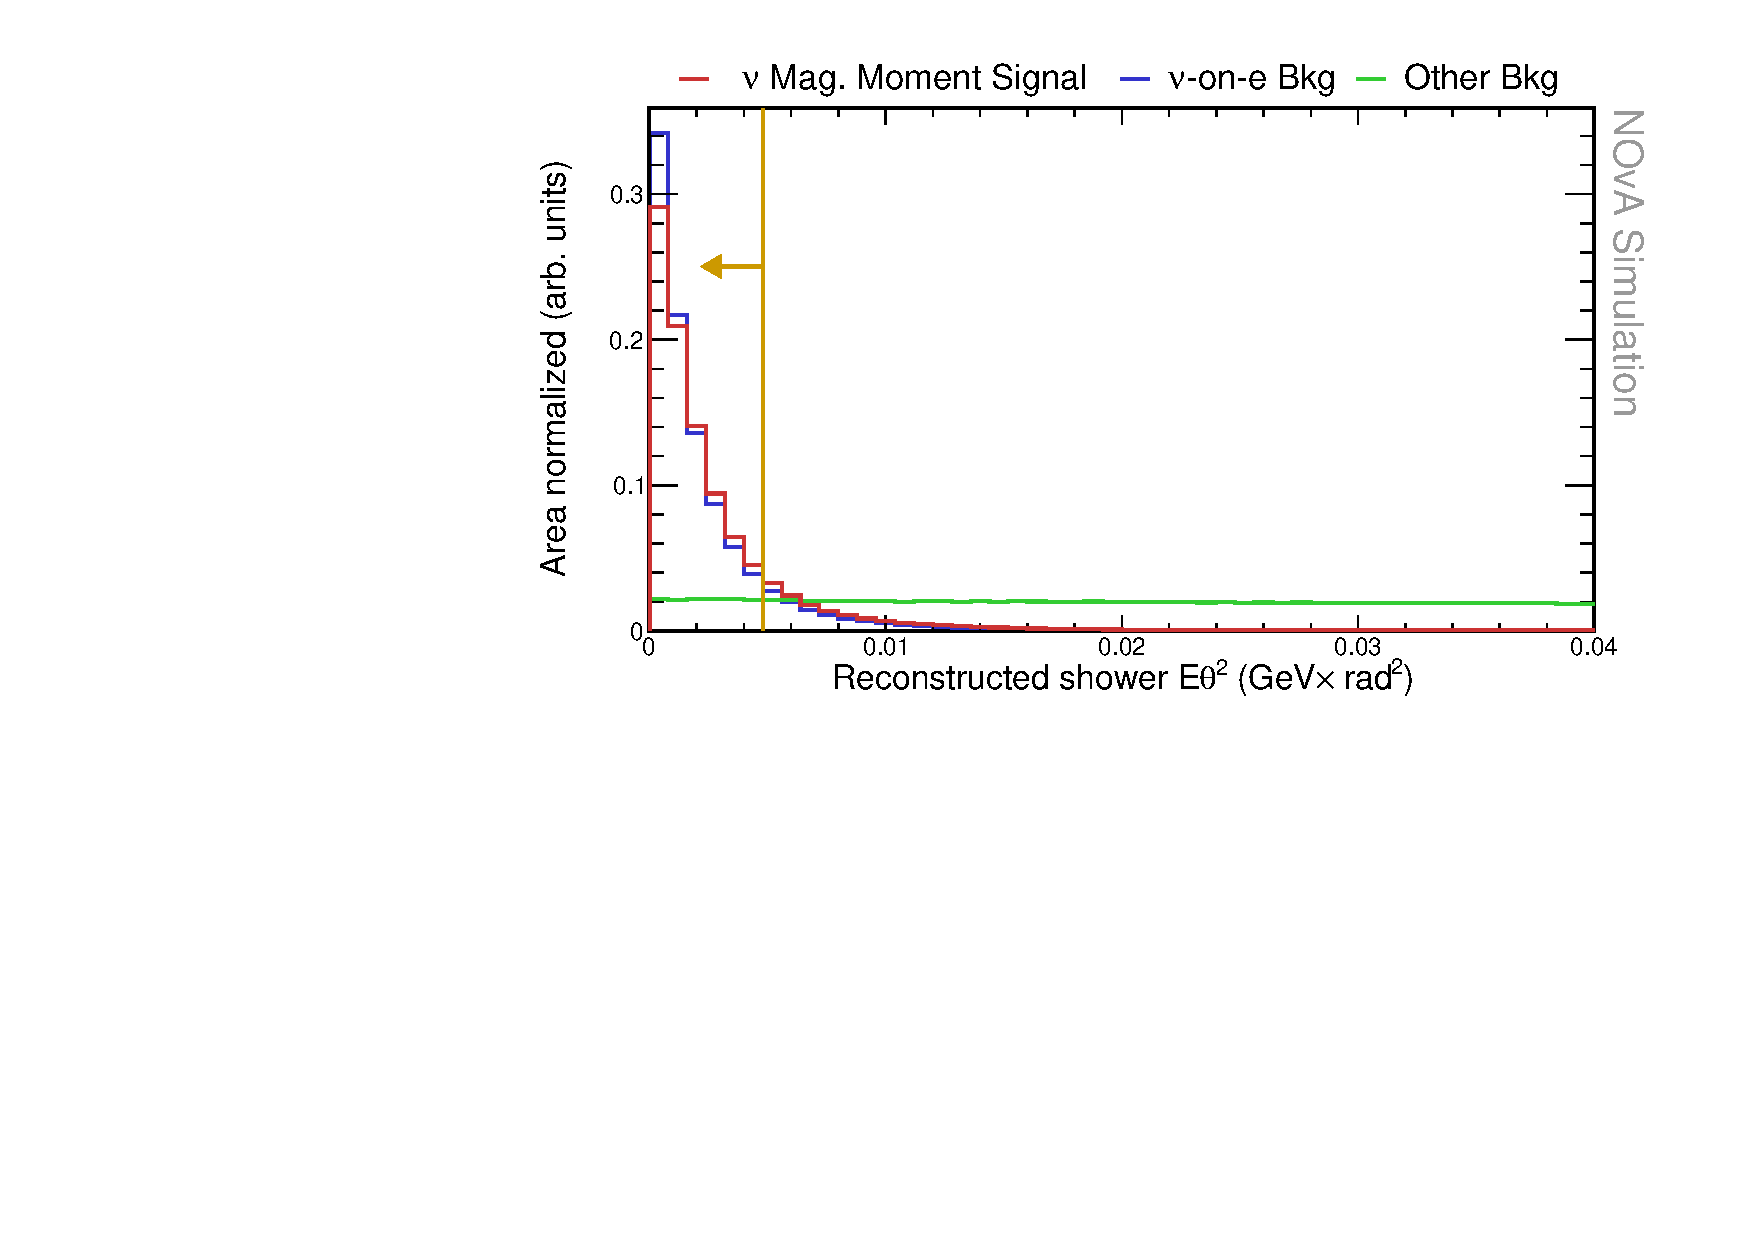
\includegraphics[width=.7\textwidth]{Plots/NuMMEventSelection/N1Cut_eth2Pre.pdf}
\caption[Reconstructed energy and $E\theta^2$ cuts]{Relative comparison of signal (red), \acrshort{nuone} background (blue), and other background (green) events in the distribution of the reconstructed energy of the primary shower (top) and of the reconstructed energy multiplied by the angle from the incoming neutrino beam direction squared.(bottom). All histograms are area-normalized. The reconstruction quality, pre-selection, fiducial and containment cuts were applied prior to making these plots. Yellow lines show the cut values on the depicted variables, with arrows pointing towards the preserved events.}
\label{fig:NuMMCutsTMVA2}
\end{figure}

\begin{figure}[hbtp]
\centering
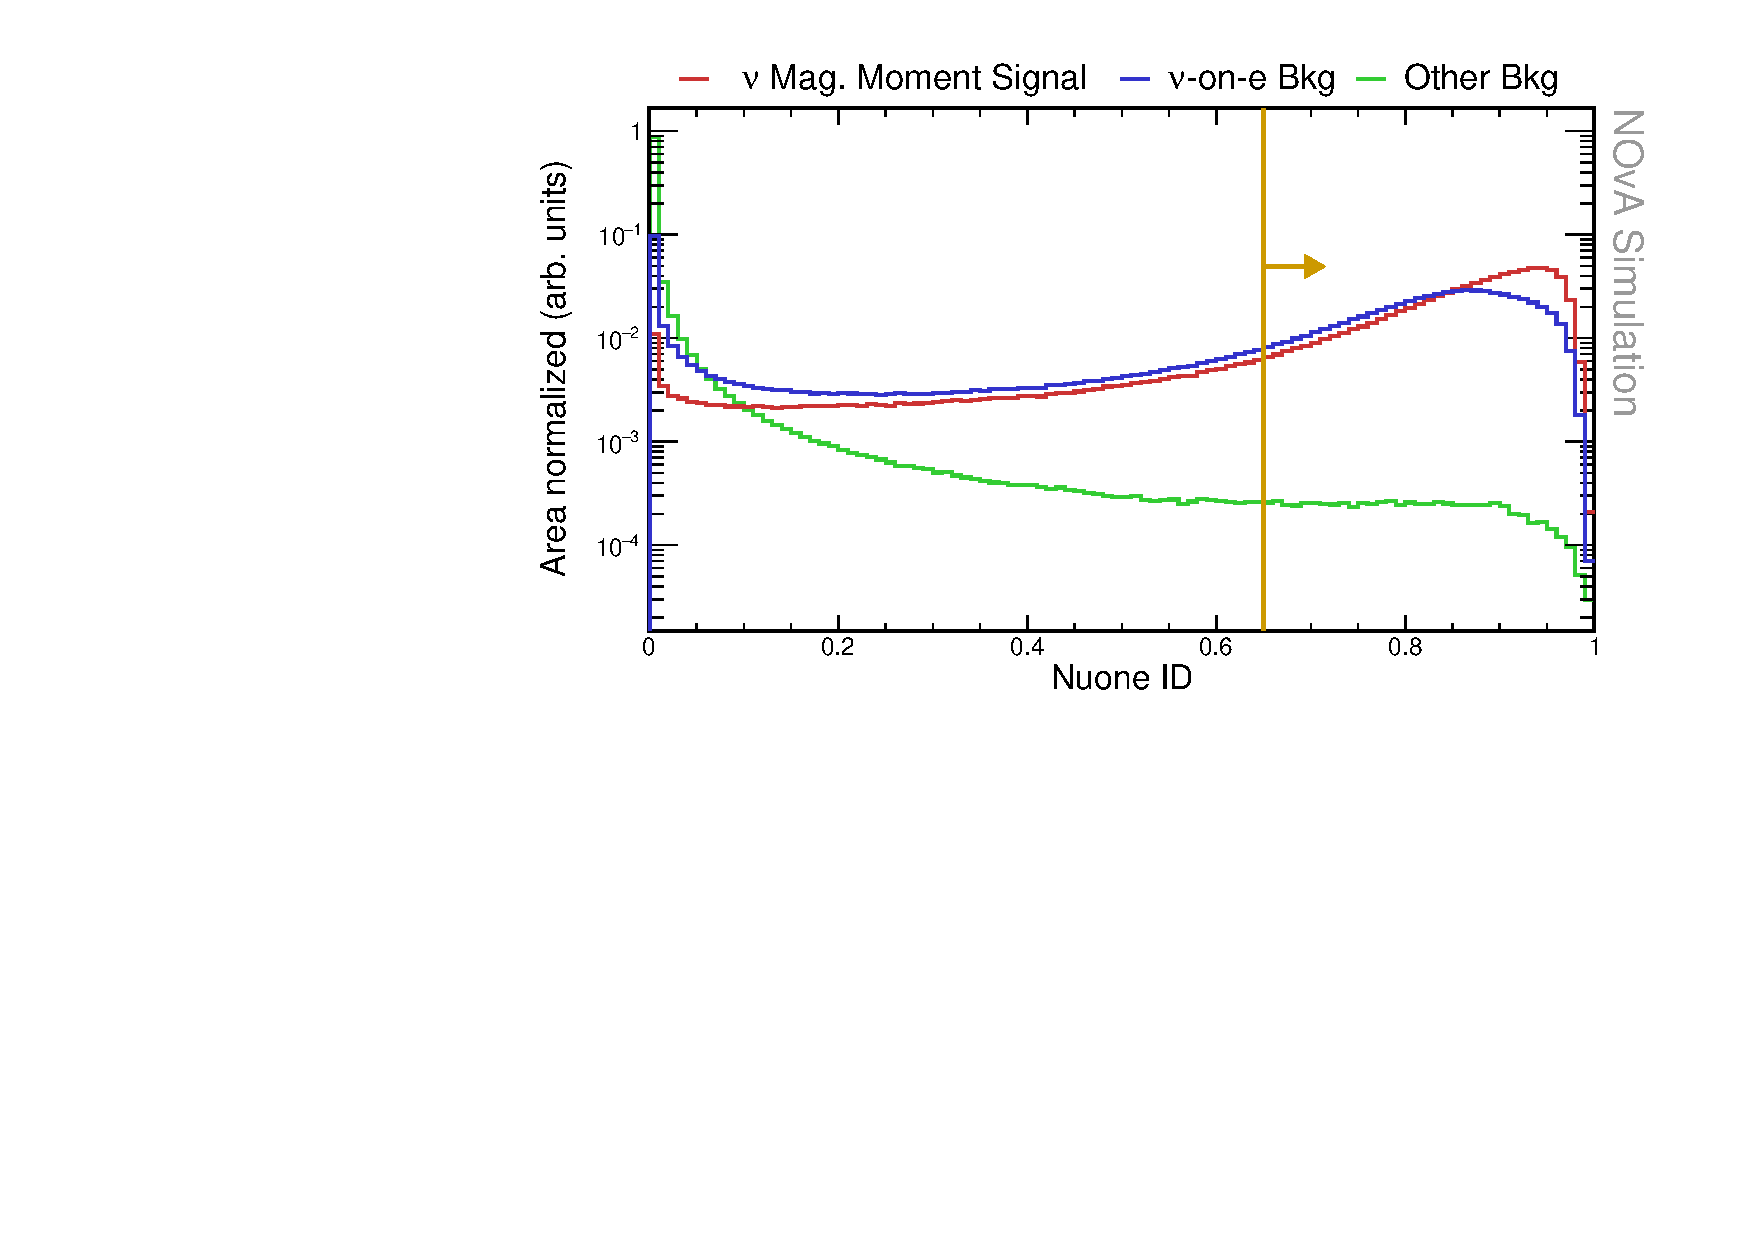
\includegraphics[width=.7\textwidth]{Plots/NuMMEventSelection/LogY_N1Cut_nuoneidPre.pdf}
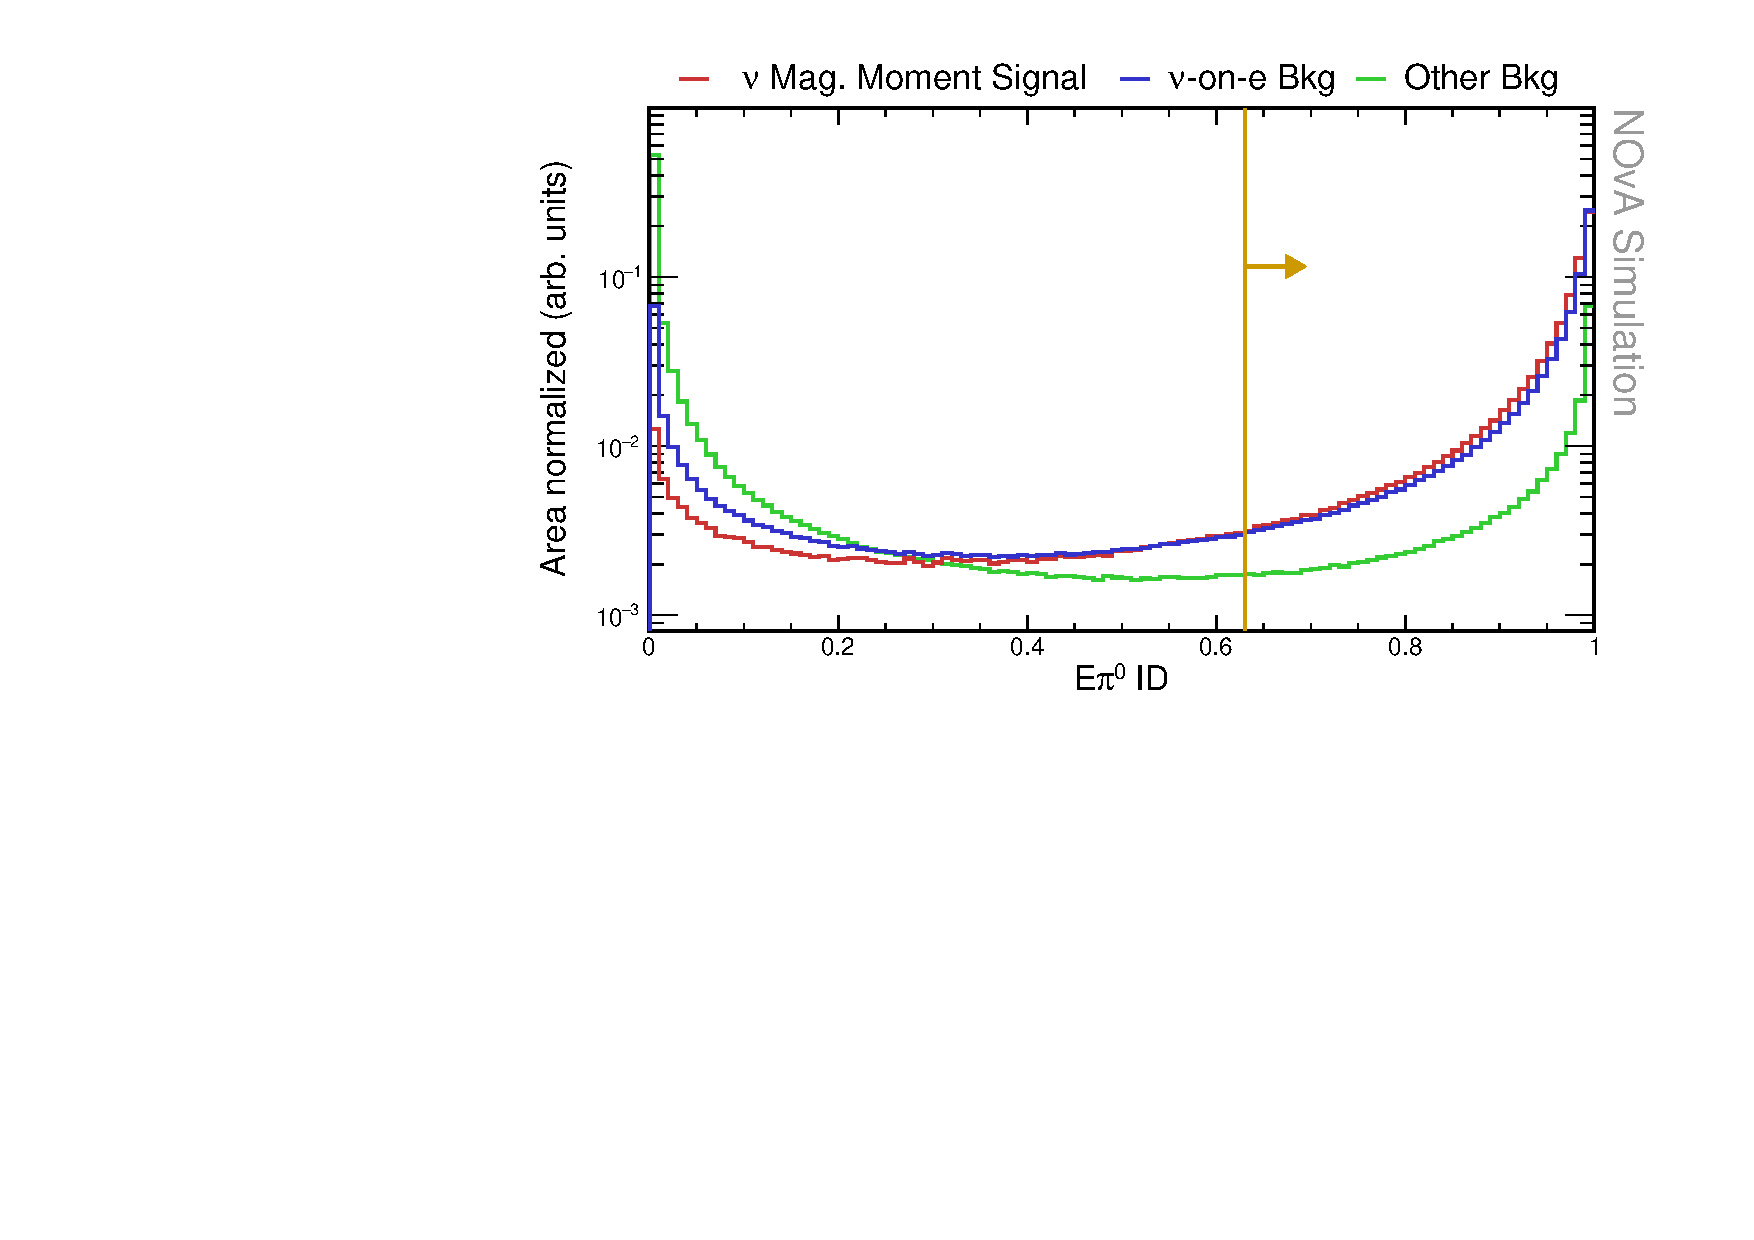
\includegraphics[width=.7\textwidth]{Plots/NuMMEventSelection/LogY_N1Cut_epi0idPre.pdf}
\caption[NuoneID and EPi0ID cuts]{Relative comparison of signal (red), \acrshort{nuone} background (blue), and other background (green) events in the distribution of the NuoneID (top) and EPi0ID (bottom) event identifiers. All histograms are area-normalized and logarithmic in the y axis. The reconstruction quality, pre-selection, fiducial and containment cuts were applied prior to making these plots. Yellow lines show the cut values on the depicted variables, with arrows pointing towards the preserved events.}
\label{fig:NuMMCutsTMVA3}
\end{figure}

\begin{table}[!hb]
\centering
\caption[Multivariate analysis cutflow table]{Event selection cutflow table for the results of the cut-based Multivariate analysis, showing the number of events and the relative efficiency of each cut for each signal sample. The relative efficiency is calculated as number of events remaining after applying the corresponding cut divided by number of event for all the previous cuts. All the cuts are listed in sequence as they are applied. The top row corresponds to the sample after applying the reconstruction quality, pre-selection, fiducial and containment cuts.}
\begin{tabular}{|l|cc|cc|cc|}\hline
\multicolumn{1}{|c|}{} & \multicolumn{2}{c|}{\textbf{Signal}} & \multicolumn{2}{c|}{\textbf{$\nu$-on-e bkg}} & \multicolumn{2}{c|}{\textbf{Other bkg}} \\
\multicolumn{1}{|c|}{\multirow{-2}{*}{\textbf{Selection}}} & \textbf{$N_{evt}$} & \textbf{$\epsilon_{rel}\left(\%\right)$} & \textbf{$N_{evt}$} & \textbf{$\epsilon_{rel}\left(\%\right)$}  & \textbf{$N_{evt}$} & \textbf{$\epsilon_{rel}\left(\%\right)$}\\\hline
\textbf{Contained} & 117.41 & 100 & 2.08$\times 10^3$ & 100 & 1.10$\times 10^6$ & 100\\
\textbf{$E_{Shower}/E_{Tot}$} & 113.03 & 96.28 & 2.02$\times 10^3$ & 97.32 & 4.53$\times 10^5$ & 41.30\\
\textbf{N$^o$ Hits} & 106.48 & 94.20 & 1.45$\times 10^3$ & 71.53 & 4.02$\times 10^5$ & 88.78\\
\textbf{High $E_{Shower}$} & 85.51 & 80.31 & 777.91 & 53.76 & 3.01$\times 10^5$ & 74.84\\
\textbf{\gls{nuone} ID} & 72.23 & 84.47 & 652.32 & 83.86 & 4.40$\times 10^3$ & 1.46\\
\textbf{$E\pi^0$ ID} & 67.35 & 93.24 & 608.19 & 93.23 & 2.83$\times 10^3$ & 64.34\\
\textbf{$E\theta^2$} & 56.80 & 84.33 & 519.09 & 85.35 & 181.24 & 6.40\\\hline
\end{tabular}
\label{tab:CutflowTableTMVA}
\end{table}

After the full event selection, the predicted number of signal events for $\mu_\nu~=~10^{-9}\mu_B$ is $56.80$, and the total number of background events under the \gls{SM} hypothesis is $700.33$. The decomposition of background into interaction types is shown in Fig.~\ref{fig:NuMMBackgroundDecomposition} and listed in Tab.~\ref{tab:NuMMBackgroundContributions}. The event selection results in
\begin{equation}
\textsf{Signal Purity}=\frac{\textsf{Signal}}{\textsf{Signal+Background}}=\unit[7.50]{\%},
\end{equation}
\begin{equation}
\textsf{Signal Efficiency}=\frac{\textsf{Signal}}{\textsf{Signal}_{\textsf{No Cut}}}=\unit[6.95]{\%}.
\end{equation}
Also,
\begin{equation}
\frac{\textsf{Signal}}{\sqrt{\textsf{Background}}}=2.15
\end{equation}
and
\begin{equation}
\textsf{\gls{FOM}}=\frac{\textsf{Signal}}{\sqrt{\textsf{Signal+Background}}}=2.06.
\end{equation}

\begin{table}[!hb]
\centering
\caption[Interactions contributing to the SM background]{Interaction types contributing to the \acrshort{SM} background after full event selection. Interactions with/without $\pi^0$ in the final state are specifically selected due to their significant contribution to the \acrshort{nuone} background.}
\begin{tabularx}{.5\textwidth}{@{}X@{}}
\textbf{Interaction} \hfill \textbf{Number of events}\\\hline
\gls{nuone} \dotfill 519.09\\
\gls{NC} w/$\pi^0$ \dotfill 72.96\\
\gls{NC} w/o $\pi^0$ \dotfill 21.51\\
$\nu_\mu$\gls{CC} w/$\pi^0$ \dotfill 28.07\\
$\nu_\mu$\gls{CC} w/o $\pi^0$ \dotfill 25.67\\
$\nu_e$\gls{CC}\gls{MEC} \dotfill 2.22\\
Other $\nu_e$\gls{CC} \dotfill 9.83\\
Other \dotfill 20.98\\\hline
\textbf{Total} \dotfill 700.33\\
\end{tabularx}
\label{tab:NuMMBackgroundContributions}
\end{table}

\begin{figure}[hbtp]
\centering
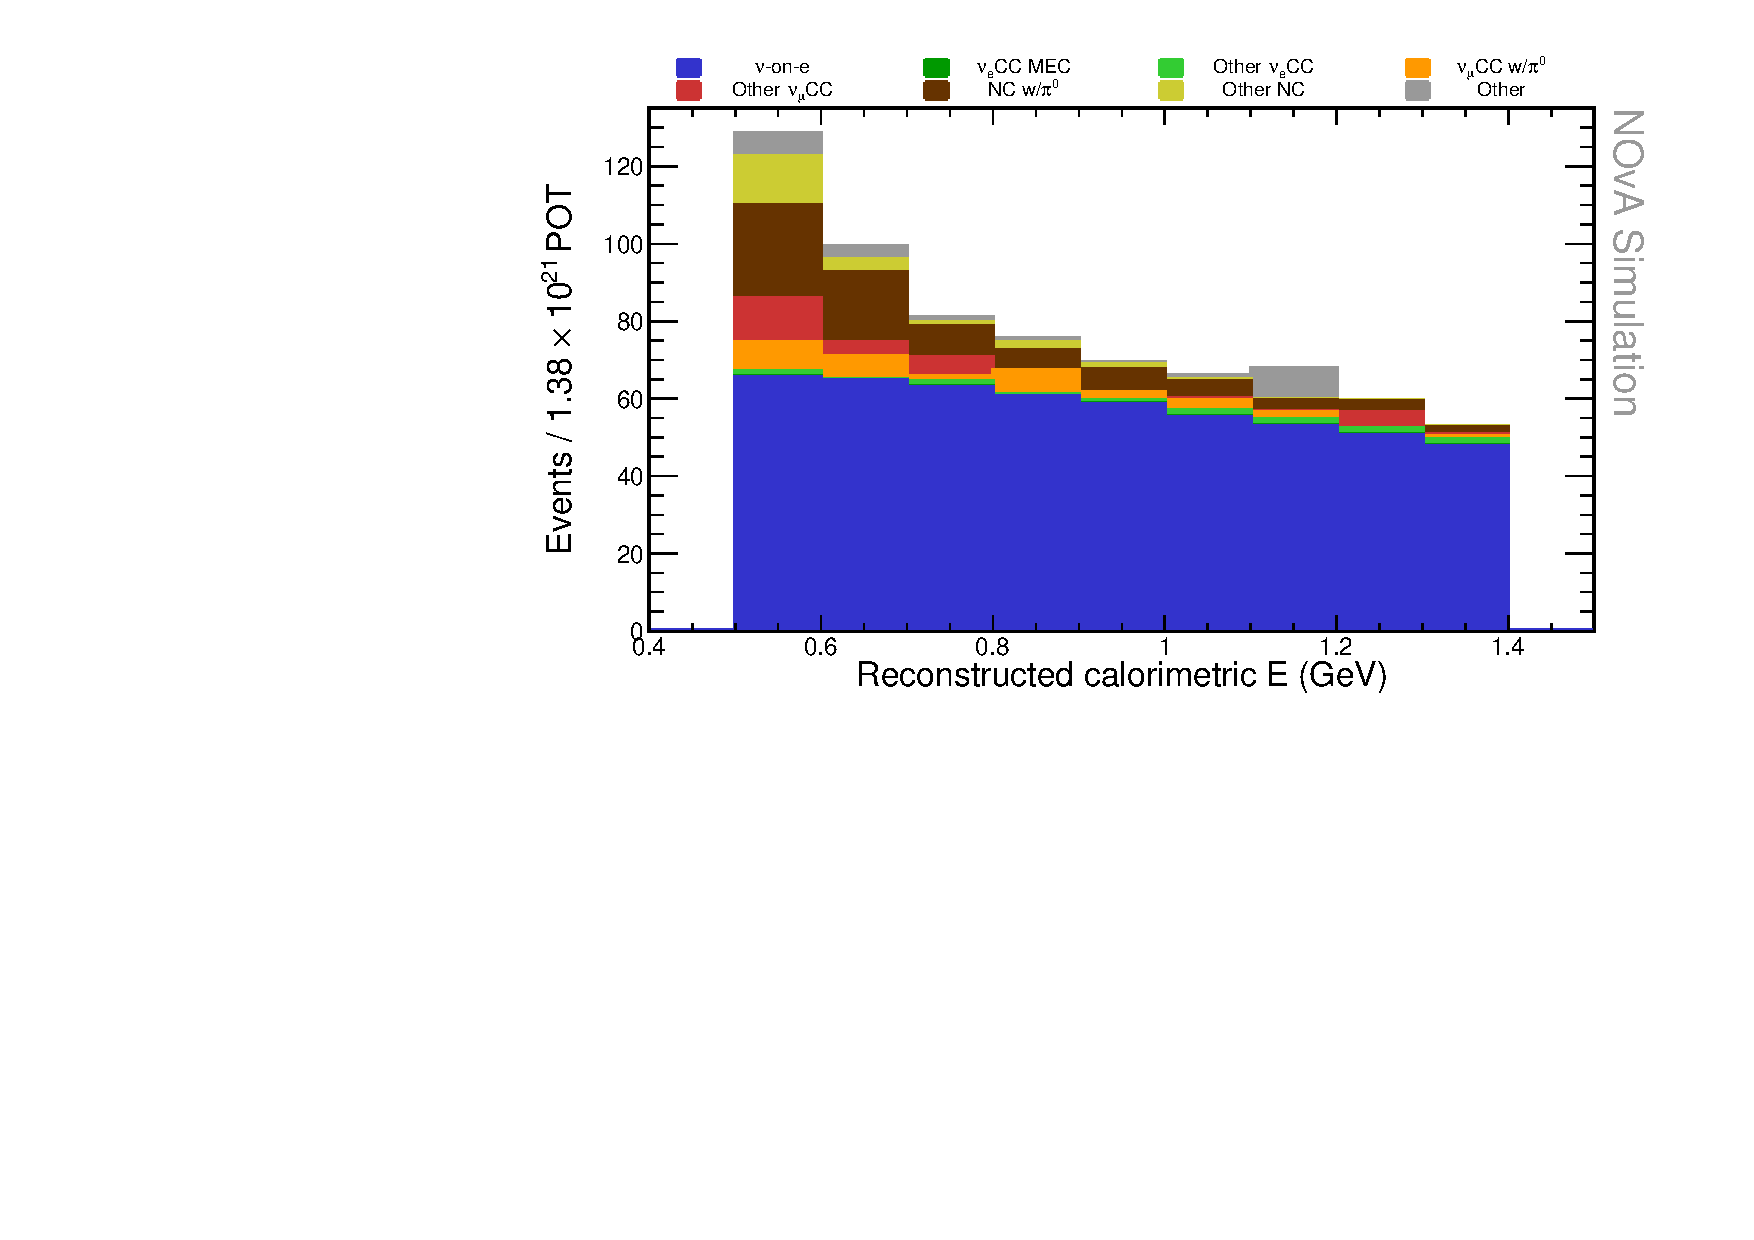
\includegraphics[width=.7\textwidth]{Plots/NuMMEventSelection/N1Cut_calESignal.pdf}
\caption[Background composition of final selection]{Background composition of events passing the full event selection as a function of the reconstructed energy of the leading shower - electron for \acrshort{nuone} events. Events are scaled to the data exposure. Origin of the "Other" background events between $\unit[1.1-1.2]{GeV}$ is not known.}
\label{fig:NuMMBackgroundDecomposition}
\end{figure}

%There are possible improvements in trying different \gls{MVA} methods, namely \gls{BDT} and so on. Since we are using the standard \gls{NOvA} simulation sample, implementation of new event identifiers into the workflow would be very complicated, unless done when updating the production. 